% !TeX program = xelatex
% !TeX encoding = UTF-8
\documentclass[UTF8,openany]{ctexbook}
\usepackage{amsmath,amssymb,amsthm}
\usepackage{tikz}
\usepackage{indentfirst}
\usepackage[a4paper,margin=25mm]{geometry}
\usepackage[unicode,hidelinks]{hyperref}
\ctexset{
  chapter = {name = {}, number = \arabic{chapter}, afterindent = true},
  section = {name = {}, number = \thechapter.\arabic{section}, afterindent = true},
  subsection = {name = {}, number = \thesection.\arabic{subsection}, afterindent = true}
}
\hypersetup{pdftitle={工科数学分析讲义},pdfsubject={极限与连续: 导数之前的内容}}
\setcounter{secnumdepth}{2}
\setlength{\parindent}{2em}
\setlength{\parskip}{0pt}
% 增大基本行距; 行内大分数较高时, 自动保留相邻行之间的净空.
\linespread{1.25}
\setlength{\lineskip}{4pt}
\setlength{\lineskiplimit}{3pt}
\newtheoremstyle{chinesetextbook}
 {0pt}{0pt}{\normalfont}{\parindent}{\bfseries}{}{1em}
 {\thmname{#1}\thmnumber{#2}\thmnote{ (#3)}}
\theoremstyle{chinesetextbook}
\newtheorem{definition}{定义}[section]
\newtheorem{example}{例}[section]
\newtheorem{theorem}{定理}[section]
\newtheorem{proposition}{命题}[section]
\newtheorem{corollary}{推论}[theorem]
\renewcommand{\thedefinition}{\arabic{definition}}
\renewcommand{\theexample}{\arabic{example}}
\renewcommand{\thetheorem}{\arabic{theorem}}
\renewcommand{\theproposition}{\arabic{proposition}}
\renewcommand{\thecorollary}{\arabic{corollary}}
\newenvironment{cnproof}{\par\indent\textbf{证明:} \ignorespaces}{\par}
\setcounter{tocdepth}{2}
% 依据: 哈尔滨工业大学数学系组编, 张传义等编, 工科数学分析(上册),
% 核对来源: 出版社样章, 2006年第五次印刷.
% https://www.ecsponline.com/yz/BE454FF85A311486E8508D66D603F800F000.pdf
% 核对来源: 出版社第1--22页试读及用户提供的第20--60页照片.
% 已核对的编号例题2.1--9.3均逐题列入, 原编号保留于题首.
% v04补入第60页例9.3与指定习题1.9第1、3、6、11题.
% 行内需要展示样式时, 统一置于完整表达式之首; 分数使用 frac.
% 精修原则: 核心概念与典型方法讲透; 非核心较难证明保留思路和必要依据.
% 方法动机: 由题目特征说明为何想到所用方法, 它解决什么困难, 并核查使用条件.
% 随学习推进, 已熟悉的运算可简写, 将解释集中于新方法和关键选择.
\newtheorem*{definitionsingle}{定义}
\newtheorem*{theoremsingle}{定理}
\newtheorem*{examplesingle}{例}
\newtheorem*{propositionsingle}{命题}
\newtheorem*{corollarysingle}{推论}
\begin{document}
\tableofcontents
\clearpage
\chapter{极限与连续}
数学分析用极限刻画变化过程, 而这些过程首先发生在实数范围内. 本章先建立集合、实数和确界的语言, 再通过数列极限逐步建立收敛理论. 随后讨论函数极限、无穷小的比较和连续性, 直至闭区间上连续函数的性质.
\section{集合与实数系}
\subsection{集合及其运算}
数学分析中的变量、函数和极限都以集合为基本语言. 使用集合时应分清两个层次: 元素是否属于集合, 以及一个集合是否包含于另一个集合.
\begin{definition}
把具有指定性质的对象汇集而成的整体称为\textbf{集合}, 组成集合的对象称为它的\textbf{元素}. 元素 $x$ 属于集合 $A$, 记作 $x\in A$; 不属于时记作 $x\notin A$. 不含任何元素的集合称为\textbf{空集}, 记作 $\varnothing$.
\end{definition}
集合可以列举元素, 也可以用性质描述, 如 $A=\{1,2,3\}$ 和 $B=\{x\in\mathbb R:x^2<1\}$. 集合不记录列举顺序, 同一元素重复写出不产生新元素. 这与下一节讨论的数列有本质区别: 数列既记录数值, 也记录位置.
\begin{definition}
若 $A$ 的每一个元素都属于 $B$, 则称 $A$ 为 $B$ 的\textbf{子集}, 记作 $A\subseteq B$. 若 $A\subseteq B$ 且 $A\ne B$, 则称 $A$ 为 $B$ 的\textbf{真子集}, 记作 $A\subsetneq B$. 若 $A\subseteq B$ 且 $B\subseteq A$, 则称两集合\textbf{相等}, 记作 $A=B$.
\end{definition}
空集是任何集合的子集, 因为“空集的每一个元素都属于 $B$”没有反例; 它是任何非空集合的真子集. 自然数集约定包含 $0$, 具体记号见下文.
\begin{definition}
设 $A,B\subseteq X$. 它们的\textbf{并集}、\textbf{交集}、\textbf{差集}及 $A$ 在全集 $X$ 中的\textbf{补集}分别为
\[
\begin{aligned}
A\cup B&=\{x:x\in A\text{ 或 }x\in B\},\\
A\cap B&=\{x:x\in A\text{ 且 }x\in B\},\\
A\setminus B&=\{x:x\in A\text{ 且 }x\notin B\},\\
A^c&=X\setminus A.
\end{aligned}
\]
\end{definition}
补集依赖所选的全集. 证明两个集合相等, 按定义就是证明两个包含关系; 证明包含关系 $A\subseteq B$, 则任取 $x\in A$, 说明 $x\in B$. 这是集合等式证明的基本格式.
\begin{example}
\textnormal{(选自教材习题1.1第1题)} 证明 $(A\cup B)\cap C=(A\cap C)\cup(B\cap C)$.
\end{example}
\par\indent\textbf{分析:} 按定义把两边元素的归属条件写出来. 左边要求 $x\in C$, 并且 $x$ 属于 $A,B$ 中至少一个; 右边要求 $x$ 属于 $A\cap C$ 或 $B\cap C$. 把“属于 $C$”分配到两种情形中, 两个条件恰好相同. 正式证明分两个包含关系书写.
\begin{cnproof}
先证左边包含于右边. 任取 $x\in(A\cup B)\cap C$, 则 $x\in C$, 且 $x\in A$ 或 $x\in B$. 若 $x\in A$, 结合 $x\in C$ 得 $x\in A\cap C$; 若 $x\in B$, 同理 $x\in B\cap C$. 两种情形都有 $x\in(A\cap C)\cup(B\cap C)$.

再证右边包含于左边. 任取 $x\in(A\cap C)\cup(B\cap C)$. 无论 $x$ 属于哪一个交集, 都有 $x\in C$, 并且 $x\in A$ 或 $x\in B$, 即 $x\in A\cup B$. 因而 $x\in(A\cup B)\cap C$. 两个包含关系都成立, 故等式成立.
\end{cnproof}
\subsection{映射与函数}
\begin{definition}
设 $X,Y$ 为非空集合. 若一个对应法则 $f$ 使每个 $x\in X$ 都有唯一确定的 $y\in Y$ 与之对应, 则称 $f$ 为从 $X$ 到 $Y$ 的\textbf{映射}, 记为 $f:X\to Y$, $y=f(x)$. 集合 $X$ 称为\textbf{定义域}, $Y$ 称为\textbf{陪域}, $f(X)=\{f(x):x\in X\}$ 称为\textbf{值域}. 元素 $y=f(x)$ 称为 $x$ 的\textbf{像}, $x$ 称为 $y$ 的一个\textbf{原像}.
\end{definition}
定义要求每个输入的像唯一, 并未要求每个输出的原像唯一, 也未要求陪域中的每个元素都有原像, 因此值域可以小于陪域. 当定义域、陪域都是数集时, 映射通常称为\textbf{函数}. 一个映射由定义域、陪域和对应法则共同确定, 只给表达式不足以确定映射.
\begin{definition}
若不同的输入必有不同的像, 即 $x_1\ne x_2$ 时 $f(x_1)\ne f(x_2)$, 则称映射为\textbf{单射}; 若 $f(X)=Y$, 即陪域中每个元素都有原像, 则称映射为\textbf{满射}; 既是单射又是满射的映射称为\textbf{双射}, 或\textbf{一一对应}.
\end{definition}
例如 $f:\mathbb R\to\mathbb R$, $f(x)=x^2$ 既非单射 ($f(-1)=f(1)$) 也非满射 ($-1$ 没有原像); 改为 $f:[0,+\infty)\to[0,+\infty)$ 后, 同一表达式确定的映射成为双射. 判断单射、满射时必须明确定义域和陪域.
\begin{definition}
设 $f:X\to Y$, $g:Y\to Z$. 由 $(g\circ f)(x)=g(f(x))$ 确定的映射 $g\circ f:X\to Z$ 称为 $f$ 与 $g$ 的\textbf{复合映射}. 若 $f$ 为单射, 则对每个 $y\in f(X)$ 恰有一个 $x\in X$ 使 $f(x)=y$, 令 $f^{-1}(y)=x$, 所得映射 $f^{-1}:f(X)\to X$ 称为 $f$ 的\textbf{逆映射}, 它满足 $f^{-1}(f(x))=x$.
\end{definition}
复合运算先作用右边的映射. 复合函数的自然定义域必须保证内层有意义, 且内层的值属于外层的定义域. 反函数记号 $f^{-1}$ 不表示倒数.
\begin{example}
\textnormal{(选自教材习题1.1第4题)} 投影 $p:\mathbb R^2\to\mathbb R$, $p(x,y)=x$ 是否为单射? 是否为满射?
\end{example}
\par\indent\textbf{分析:} 判断满射, 要从陪域中任取一个数 $t$, 看能否解出原像, 即解方程 $p(x,y)=t$. 判断单射, 要看不同的输入是否可能有相同的像; 要否定单射, 只需找到一对不同的输入, 它们的像相同. 投影只保留第一个坐标, 第二个坐标不影响结果, 这既使方程容易求解, 也提示了反例的构造.
\begin{cnproof}
任取 $t\in\mathbb R$. 方程 $p(x,y)=x=t$ 的解为 $x=t$, $y$ 任意, 例如 $(t,0)\in\mathbb R^2$ 满足 $p(t,0)=t$. 每个 $t$ 都有原像, 故 $p$ 是满射.

另一方面, $(0,0)\ne(0,1)$, 但 $p(0,0)=0=p(0,1)$. 不同的输入有相同的像, 故 $p$ 不是单射.
\end{cnproof}
\subsection{实数、区间和绝对值}
本书采用 $\mathbb N=\{0,1,2,\ldots\}$, $\mathbb N^+=\{1,2,3,\ldots\}$, 并用 $\mathbb Z,\mathbb Q,\mathbb R$ 分别表示整数集、有理数集和实数集. 有理数可写为 $\displaystyle\frac pq$, 其中 $p\in\mathbb Z$, $q\in\mathbb N^+$. 实数中不是有理数的数称为\textbf{无理数}.

实数与数轴上的点一一对应, 可以比较大小. 设 $a<b$, 常用区间为
\[
\begin{aligned}
(a,b)&=\{x:a<x<b\},& [a,b]&=\{x:a\le x\le b\},\\
[a,b)&=\{x:a\le x<b\},& (a,b]&=\{x:a<x\le b\}.
\end{aligned}
\]
端点处用方括号表示包含端点, 用圆括号表示不包含端点. 无穷区间如 $(a,+\infty)$、$(-\infty,b]$ 和 $\mathbb R=(-\infty,+\infty)$ 中, $\pm\infty$ 是描述无界方向的符号, 不是实数, 也不是区间的端点.
\begin{definition}
实数 $x$ 的\textbf{绝对值}为
\[
|x|=\begin{cases}x,&x\ge0,\\-x,&x<0.\end{cases}
\]
$|x-y|$ 表示数轴上 $x,y$ 两点之间的距离.
\end{definition}
由定义直接得到: $|x|\ge0$; $|x|=0$ 当且仅当 $x=0$; $|xy|=|x|\,|y|$; 对 $M\ge0$, 条件 $|t|\le M$ 等价于 $-M\le t\le M$, 条件 $|t|<M$ 等价于 $-M<t<M$. 最后一条把绝对值不等式化为两个普通不等式, 是估计绝对值时最常用的工具.
\begin{theorem}[三角不等式]
对任意实数 $a,b,c$, 有
\[
|a+b|\le|a|+|b|,\qquad |a-b|\le|a-c|+|c-b|,
\]
以及反三角不等式 $\bigl||a|-|b|\bigr|\le|a-b|$.
\end{theorem}
\par\indent\textbf{分析:} 第一式的左边是一个和的绝对值. 要估计 $|a+b|$, 按上面的等价表述, 只需从两侧估计 $a+b$, 即证明 $-(|a|+|b|)\le a+b\le|a|+|b|$; 而 $a,b$ 各自满足 $-|a|\le a\le|a|$, $-|b|\le b\le|b|$, 相加即可. 第二式要把距离 $|a-b|$ 与经过中间点 $c$ 的两段距离联系起来, 在 $a-b$ 中加入再减去 $c$ 就出现了这两段. 第三式要估计 $|a|-|b|$ 的绝对值, 需要同时得到 $|a|-|b|$ 的上界和下界; 把 $a$ 写成 $(a-b)+b$ 用第一式得到上界, 交换 $a,b$ 的位置得到下界.
\begin{cnproof}
先证第一式. 由绝对值的定义,
\[
-|a|\le a\le|a|,\qquad -|b|\le b\le|b|.
\]
两个下界相加, 两个上界相加, 得
\[
-(|a|+|b|)\le a+b\le|a|+|b|.
\]
由于 $|a|+|b|\ge0$, 这等价于 $|a+b|\le|a|+|b|$.

第二式中, 由 $a-b=(a-c)+(c-b)$, 对右边两个加数用第一式, 得 $|a-b|\le|a-c|+|c-b|$.

最后证反三角不等式. 由 $a=(a-b)+b$ 及第一式, $|a|\le|a-b|+|b|$, 即
\[
|a|-|b|\le|a-b|.
\]
交换 $a,b$ 的位置, 因 $|b-a|=|a-b|$, 得 $|b|-|a|\le|a-b|$, 即 $-|a-b|\le|a|-|b|$. 两式合起来是
\[
-|a-b|\le|a|-|b|\le|a-b|,
\]
由绝对值不等式的等价表述, 这就是 $\bigl||a|-|b|\bigr|\le|a-b|$.
\end{cnproof}
三角不等式把一个难以直接控制的距离拆成几段容易控制的距离. 后面证明极限的唯一性、运算法则和柯西准则时都要用它; 反三角不等式则用于从 $|a_n-a|$ 小推出 $|a_n|$ 与 $|a|$ 接近.
\subsection{邻域}
\begin{definition}
设 $x_0\in\mathbb R$, $r>0$. 开区间
\[
U(x_0,r)=(x_0-r,x_0+r)=\{x:|x-x_0|<r\}
\]
称为 $x_0$ 的 \textbf{$r$ 邻域}; 集合
\[
\mathring U(x_0,r)=\{x:0<|x-x_0|<r\}
\]
称为 $x_0$ 的 \textbf{$r$ 去心邻域}.
\end{definition}
邻域包含中心点, 去心邻域不包含中心点. 半径越小, 对应的距离限制越严格. 数列极限只用普通邻域, 因为数列的项允许等于极限; 函数极限要排除中心点本身, 将用到去心邻域.
\subsection{有界集与确界}
\begin{definition}
设 $A\subseteq\mathbb R$ 非空. 若存在实数 $M$, 使每个 $x\in A$ 都满足 $x\le M$, 则称 $A$ \textbf{有上界}, $M$ 称为 $A$ 的一个\textbf{上界}. 若存在实数 $m$, 使每个 $x\in A$ 都满足 $x\ge m$, 则称 $A$ \textbf{有下界}, $m$ 称为一个\textbf{下界}. 既有上界又有下界的集合称为\textbf{有界集}.
\end{definition}
上界和下界不要求属于集合, 也不唯一: 若 $M$ 是上界, 任何大于 $M$ 的数也是上界. 若 $M\in A$ 且 $M$ 是 $A$ 的上界, 则称 $M$ 为 $A$ 的\textbf{最大元素}; 最小元素类似定义. 最大、最小元素必须属于集合, 上、下界则不必. 有上界的集合未必有最大元素, 例如 $(0,1)$; 在所有上界中寻找最小的一个, 就得到确界的概念.
\begin{definition}
设 $A\subseteq\mathbb R$ 非空. 若 $A$ 的所有上界中有最小者, 则称它为 $A$ 的\textbf{上确界}, 记为 $\sup A$. 若 $A$ 的所有下界中有最大者, 则称它为 $A$ 的\textbf{下确界}, 记为 $\inf A$.
\end{definition}
\par\indent\textbf{公理 (确界原理)} 每个非空且有上界的实数集都有上确界.

这是实数系\textbf{完备性}的一种表述, 本章以它为出发点. 有理数系不具有这一性质: 在有理数范围内, 集合 $\{x\in\mathbb Q:x>0,\ x^2<2\}$ 非空有上界, 却没有有理数作为最小上界. 当 $A$ 有最大元素时, 最大元素就是上确界; 一般情况下上确界可以不属于 $A$.
\begin{theorem}[确界的刻画]
设 $A\subseteq\mathbb R$ 非空, $s\in\mathbb R$. 则 $s=\sup A$ 的充分必要条件是以下两点同时成立: 每个 $x\in A$ 都满足 $x\le s$; 对任意 $\varepsilon>0$, 存在 $x_\varepsilon\in A$, 使 $x_\varepsilon>s-\varepsilon$.
\end{theorem}
\par\indent\textbf{分析:} 第一点说 $s$ 是上界, 第二点说 $A$ 的元素可以从下方任意接近 $s$. 定理把“最小上界”翻译成可以逐项验证的条件, 以后用确界时总是通过这两点. 证明的要点是把“$s$ 是最小上界”换个说法: 任何比 $s$ 小的数都不是上界, 而“$u$ 不是上界”意味着 $A$ 中有元素超过 $u$. 从 $s=\sup A$ 推第二点, 取 $u=s-\varepsilon$; 从第二点推最小性, 对任意 $u<s$ 取 $\varepsilon=s-u$, 第二点就给出超过 $u$ 的元素.
\begin{cnproof}
先设 $s=\sup A$. 因 $s$ 是上界, 第一点成立. 任给 $\varepsilon>0$, 由于 $s-\varepsilon<s$, 而 $s$ 是最小的上界, $s-\varepsilon$ 不是上界, 即并非所有元素都不超过它; 于是存在 $x_\varepsilon\in A$, 使 $x_\varepsilon>s-\varepsilon$. 第二点成立.

反过来, 设两点都成立. 由第一点, $s$ 是上界. 任取 $u<s$, 令 $\varepsilon=s-u>0$, 由第二点存在 $x_\varepsilon\in A$, 使 $x_\varepsilon>s-\varepsilon=u$, 所以 $u$ 不是上界. 由于每个小于 $s$ 的数都不是上界, $s$ 是最小的上界, 即 $s=\sup A$.
\end{cnproof}
第二点中的 $x_\varepsilon$ 可以等于 $s$, 这对应上确界属于 $A$ 的情形. 对下确界有对称的刻画: $t=\inf A$ 当且仅当 $t$ 是下界, 且对任意 $\varepsilon>0$ 存在 $x\in A$ 使 $x<t+\varepsilon$.
\begin{corollarysingle}
非空且有下界的实数集必有下确界. 对非空有下界的集合 $A$, 有 $\inf A=-\sup(-A)$, 其中 $-A=\{-x:x\in A\}$.
\end{corollarysingle}
\par\indent\textbf{分析:} 确界原理只保证上确界的存在. 把集合中每个数取相反数, 所有不等号反向, 下界就变成上界, 于是下界问题可转化为上界问题.
\begin{cnproof}
设 $l$ 为 $A$ 的一个下界. 对所有 $x\in A$ 有 $x\ge l$, 即 $-x\le-l$, 所以 $-l$ 是 $-A$ 的上界. $-A$ 非空有上界, 由确界原理, $s=\sup(-A)$ 存在. 下面证明 $-s=\inf A$.

对任意 $x\in A$, 有 $-x\in-A$, 故 $-x\le s$, 即 $x\ge-s$, 所以 $-s$ 是 $A$ 的下界. 任取 $v>-s$, 则 $-v<s$; 由 $s$ 是 $-A$ 的最小上界, $-v$ 不是 $-A$ 的上界, 存在 $y\in-A$ 使 $y>-v$. 令 $x=-y\in A$, 则 $x<v$, 所以 $v$ 不是 $A$ 的下界. 因此 $-s$ 是最大的下界, 即 $\inf A=-s=-\sup(-A)$.
\end{cnproof}
\begin{theorem}[阿基米德性质]
正整数集没有上界. 等价地, 对任意实数 $t$, 存在正整数 $n>t$.
\end{theorem}
\par\indent\textbf{分析:} 结论看似显然, 但“对任意实数都能找到更大的正整数”涉及全部实数, 需要从实数的公理推出. 用反证: 若正整数集有上界, 确界原理给出它的上确界 $s$. 由确界的刻画, 对 $\varepsilon=1$ 存在正整数 $n>s-1$; 取 $s-1$ 是为了加 $1$ 之后得到一个超过 $s$ 的正整数, 这与 $s$ 是上界矛盾.
\begin{cnproof}
反设正整数集 $\mathbb N^+$ 有上界. 它非空, 由确界原理有上确界 $s$. 由确界的刻画, 对 $\varepsilon=1$ 存在正整数 $n>s-1$. 则 $n+1$ 仍是正整数, 且 $n+1>s$, 与 $s$ 是 $\mathbb N^+$ 的上界矛盾. 故 $\mathbb N^+$ 没有上界, 即对任意实数 $t$ 存在正整数 $n>t$.
\end{cnproof}
下面的确界例题和稠密性证明中, “选取充分大的正整数”这一步都以阿基米德性质为依据; 下一节数列极限定义中选取分界下标时也要用它.
\begin{example}
\textnormal{(选自教材习题1.1第8题)} 求 $\displaystyle A=\left\{\frac1n:n\ge2,\ n\in\mathbb N^+\right\}$ 的上确界与下确界, 并判断它们是否属于 $A$.
\end{example}
\par\indent\textbf{分析:} 先观察元素的范围, 找出一个上界和一个下界; 再按确界的刻画验证它们不能再收紧. 对上界, 若它恰好是集合的元素, 就是最大元素, 自然是上确界. 对下界 $0$, 它不属于 $A$, 要用刻画的第二点: 对任意 $\varepsilon>0$ 找一个小于 $\varepsilon$ 的元素, 即解不等式 $\displaystyle\frac1n<\varepsilon$, 并保证所选 $n$ 满足 $n\ge2$.
\begin{cnproof}
因为 $n\ge2$, 且正数的倒数随分母增大而减小, 所以每个元素满足
\[
0<\frac1n\le\frac12.
\]
故 $\displaystyle\frac12$ 是上界, $0$ 是下界.

$n=2$ 时 $\displaystyle\frac12\in A$, 它是 $A$ 的最大元素, 因而 $\displaystyle\sup A=\frac12$, 上确界属于 $A$.

对下界, $0$ 是下界, 再验证刻画的第二点. 任给 $\varepsilon>0$, 要找 $n\ge2$ 使 $\displaystyle\frac1n<\varepsilon$, 即 $\displaystyle n>\frac1\varepsilon$. 由阿基米德性质, 存在正整数 $\displaystyle n>\max\left\{2,\frac1\varepsilon\right\}$, 此时 $\displaystyle\frac1n\in A$ 且 $\displaystyle\frac1n<\varepsilon=0+\varepsilon$. 所以 $\inf A=0$. 由于每个元素都严格大于 $0$, 下确界不属于 $A$; $A$ 没有最小元素.
\end{cnproof}
\subsection{补充证明: 平方根二的无理性}
\begin{propositionsingle}
$\sqrt2$ 为无理数.
\end{propositionsingle}
\begin{cnproof}
反设 $\displaystyle\sqrt2=\frac pq$, 其中 $p,q$ 为互素的正整数; 任何正有理数都可以约分成这种形式. 平方得 $p^2=2q^2$, 因而 $p^2$ 为偶数. 奇数的平方是奇数, 所以 $p$ 必为偶数. 令 $p=2k$, 代回得 $4k^2=2q^2$, 即 $q^2=2k^2$, 同理 $q$ 也为偶数. 于是 $p,q$ 有公因子 $2$, 与互素矛盾. 故 $\sqrt2$ 是无理数.
\end{cnproof}
\subsection{实数的稠密性}
有理数在实数中\textbf{稠密}, 指任意两个不同实数之间都有有理数; 无理数也有同样的性质. 这不是说每个实数都是有理数, 而是说再短的非空开区间也不会只含其中一类数.
\begin{theorem}[有理数与无理数的稠密性]
任意非空开区间 $(a,b)$ 内既有有理数, 也有无理数.
\end{theorem}
\par\indent\textbf{分析:} 有理数具有 $\displaystyle\frac km$ 的形式, 要找 $(a,b)$ 内的有理数, 就是找正整数 $m$ 和整数 $k$, 使 $\displaystyle a<\frac km<b$, 即 $ma<k<mb$. 这把问题转化为: 区间 $(ma,mb)$ 内是否有整数. 区间 $(a,b)$ 可能很短, 其中未必有整数; 但乘以 $m$ 后长度变为 $m(b-a)$, 只要它大于 $1$, 其中就一定有整数. 阿基米德性质保证这样的 $m$ 存在. 找无理数时, 利用已证的 $\sqrt2$ 是无理数以及“有理数加无理数仍是无理数”: 先在平移后的区间 $(a-\sqrt2,b-\sqrt2)$ 内取有理数 $r$, 则 $r+\sqrt2$ 就是 $(a,b)$ 内的无理数.
\begin{cnproof}
先找有理数. 由阿基米德性质, 取正整数 $m$ 满足 $\displaystyle m>\frac1{b-a}$, 则 $mb-ma=m(b-a)>1$. 由阿基米德性质, 大于 $ma$ 的整数存在, 取其中最小者为 $k$, 则 $ma<k\le ma+1$; 又 $ma+1<mb$, 所以
\[
ma<k<mb.
\]
由于 $m>0$, 各项除以 $m$ 不改变不等号方向, 得 $\displaystyle a<\frac km<b$, 这就是所需的有理数.

再找无理数. 区间 $(a-\sqrt2,b-\sqrt2)$ 的长度仍为 $b-a>0$, 由刚证的结论, 其中有有理数 $r$, 于是 $a<r+\sqrt2<b$. 若 $r+\sqrt2$ 是有理数, 则 $\sqrt2=(r+\sqrt2)-r$ 是两个有理数之差, 也是有理数, 与上一小节矛盾. 故 $r+\sqrt2$ 是 $(a,b)$ 内的无理数.
\end{cnproof}
\section{数列与极限}

\subsection{数列}

\begin{definition}
按正整数的先后顺序排列的一列实数
\[
a_1,a_2,\ldots,a_n,\ldots
\]
称为\textbf{数列}, 记作 $\{a_n\}_{n=1}^{\infty}$ 或 $\{a_n\}$. 其中每一个数称为数列的\textbf{项}, 第 $n$ 项 $a_n$ 称为数列的\textbf{通项}.
\end{definition}

数列既规定各项的数值, 也规定各项的位置, 同一个数可以在不同位置反复出现. 例如数列 $1,0,1,0,\ldots$ 只有两个不同的取值, 却有无限多项. 因此数列的记号虽然使用花括号, 却不能理解为由各项组成的数集.

给定通项就能确定每一项. 例如 $a_n=2^{-n}$ 给出数列
\[
\frac12,\frac14,\frac18,\ldots,
\]
而 $\displaystyle a_n=\frac{(-1)^{n+1}}{n}$ 给出数列
\[
1,-\frac12,\frac13,-\frac14,\ldots.
\]
数列也可以看作\textbf{以正整数集为定义域的函数} $f:\mathbb N^+\to\mathbb R$, $f(n)=a_n$. 这里使用 $\mathbb N^+$, 是因为本书的自然数集包含 $0$, 而数列从 $a_1$ 开始编号.

研究数列的主要问题, 是下标不断增大时各项呈现怎样的变化趋势. 上面两个数列的变化方式不同: 前者始终为正并逐渐减小, 后者正负交替, 但二者的各项都越来越接近 $0$. 数列 $1,0,1,0,\ldots$ 始终在两个数之间交替, 数列 $1,2,3,\ldots$ 则不断增大. 要准确区分这些情形, 就需要数列极限的概念.

\subsection{数列极限}

先用距离描述接近程度. 数 $a_n$ 与实数 $a$ 的距离为 $|a_n-a|$. 规定这一距离小于某个正数 $\varepsilon$, 就是要求
\[
|a_n-a|<\varepsilon,\qquad\text{即}\quad a-\varepsilon<a_n<a+\varepsilon,
\]
也就是 $a_n$ 落在上一节定义的邻域 $U(a,\varepsilon)$ 中.

“各项越来越接近 $a$”并不要求它们恰好等于 $a$, 也不要求距离逐项减小. 所需要的是: 无论给定多小的正数 $\varepsilon$, 从某一项以后, 所有项与 $a$ 的距离都小于 $\varepsilon$.

\begin{definition}
设 $\{a_n\}$ 为一数列, $a$ 为实数. 若对任意给定的 $\varepsilon>0$, 均存在自然数 $N$, 使当 $n>N$ 时恒有
\[
|a_n-a|<\varepsilon,
\]
则称数列 $\{a_n\}$ \textbf{收敛于} $a$, 并称 $a$ 为该数列的\textbf{极限}, 记为
\[
\lim_{n\to\infty}a_n=a,
\]
或记为 $a_n\to a\ (n\to\infty)$. 不收敛于任何实数的数列称为\textbf{发散数列}.
\end{definition}

这一定义通常称为数列极限的 $\varepsilon$-$N$ 定义. 其中 $\varepsilon$ 刻画允许的误差, $N$ 刻画从哪一项起误差满足要求. 定义的逻辑结构是: 对每一个 $\varepsilon>0$ 都要找到相应的 $N$. $N$ 在 $\varepsilon$ 给定之后选取, 可以随 $\varepsilon$ 改变, 有时记作 $N(\varepsilon)$; $N$ 选定后, 对每一个 $n>N$ 都要检查误差要求, 因而 \textbf{$N$ 不能再随 $n$ 改变}. 分界之前的项可以满足要求, 也可以不满足, 定义对此不作限制.

因此收敛还可以表述为: 对 $a$ 的任意邻域 $U(a,\varepsilon)$, 数列中至多有有限项落在该邻域之外. 这里按项的位置计数, 相同的数值在不同位置出现时算作不同的项.

有两点需要分清. 其一, 只对某些具体的误差验证不够: 证明了误差最终小于 $0.01$, 并不能说明它最终小于 $0.001$, 定义要求同一论证对所有正误差都有效. 其二, 只有无限多项满足误差要求也不够: $(-1)^n$ 有无限多项等于 $1$, 但它不收敛于 $1$, 因为其余的项与 $1$ 的距离始终为 $2$. 定义要求的是越过分界之后的所有项都满足要求.

寻找 $N$ 时, 通常先在草稿中从目标 $|a_n-a|<\varepsilon$ 反推 $n$ 应满足的条件; 正式证明则按定义的顺序书写, 先给出 $N$, 再由 $n>N$ 正向推出误差小于 $\varepsilon$. 反推只需找到充分条件, 不要求每一步等价, 也不要求 $N$ 最小: 若某个 $N$ 有效, 任何更大的自然数也有效.

还应区分两个命题: 数列不收敛于某个给定的 $a$, 与数列发散. 前者只否定一个候选极限. 将定义中的量词和不等式逐一否定, 可得它的准确表述:
\[
\exists\,\varepsilon_0>0,\quad
\forall\,N\in\mathbb N,\quad
\exists\,n\in\mathbb N^+:\quad
n>N,\quad |a_n-a|\ge\varepsilon_0.
\]
其中 $\forall$ 表示“任意”, $\exists$ 表示“存在”. 否定后, 坏的误差 $\varepsilon_0$ 是固定的, 坏的下标 $n$ 则可以随 $N$ 改变. 要证明数列发散, 需要说明每一个实数都不是它的极限. 发散不等于各项无限增大, 在不同数值之间持续振荡同样导致发散.

本书用方括号 $[t]$ 表示\textbf{不超过 $t$ 的最大整数}, 即
\[
[t]\le t<[t]+1.
\]
当 $t\ge0$ 时, $[t]\in\mathbb N$. 若 $n$ 为整数且 $n>[t]$, 则 $n\ge[t]+1>t$. 因此, 推得只需 $n>t$ 后, 可以直接取 $N=[t]$, 不必再加 $1$, 本书统一采用这一取法. 为允许取整结果为 $0$, 极限定义中的分界下标 $N$ 取自 $\mathbb N$; 数列下标 $n$ 仍取自 $\mathbb N^+$. 这一约定与要求 $N$ 为正整数的定义等价.

以下例题从简单的误差估计开始, 再讨论需要分拆求和或引入辅助量的情形.

\begin{example}
\textnormal{(教材例2.1)} 求证
\[
\lim_{n\to\infty}\frac{n+1}{n}=1.
\]
\end{example}

\par\indent\textbf{分析:} 按定义, 要对任意给定的 $\varepsilon>0$ 找到 $N$, 使 $n>N$ 时通项与 $1$ 的距离小于 $\varepsilon$. 先算出这个距离:
\[
\left|\frac{n+1}{n}-1\right|=\frac1n.
\]
目标变为 $\displaystyle\frac1n<\varepsilon$. 因为 $n,\varepsilon$ 都为正, 它等价于 $\displaystyle n>\frac1\varepsilon$, 这就是下标应满足的条件. 定义要求给出的是自然数 $N$, 而 $\displaystyle\frac1\varepsilon$ 未必为整数; 按取整约定取 $\displaystyle N=\left[\frac1\varepsilon\right]$, 每个整数 $n>N$ 都严格超过 $\displaystyle\frac1\varepsilon$. 注意要求的是后面的 $n$ 超过这一阈值, 不要求 $N$ 自身超过它.

\begin{cnproof}
任给 $\varepsilon>0$, 取自然数
\[
N=\left[\frac1\varepsilon\right].
\]
由取整记号的性质, 对任意正整数 $n>N$ 都有 $\displaystyle n>\frac1\varepsilon$, 从而
\[
\left|\frac{n+1}{n}-1\right|=\frac1n<\varepsilon.
\]
故由定义, $\displaystyle\lim_{n\to\infty}\frac{n+1}{n}=1$.
\end{cnproof}

答题时上述证明可以简写为: 任给 $\varepsilon>0$, 取 $\displaystyle N=\left[\frac1\varepsilon\right]$. 当 $n>N$ 时, $\displaystyle\left|\frac{n+1}{n}-1\right|=\frac1n<\varepsilon$. 故 $\displaystyle\lim_{n\to\infty}\frac{n+1}{n}=1$.

当 $\varepsilon>1$ 时, $\displaystyle N=\left[\frac1\varepsilon\right]=0$, 表示从第一项起已满足误差要求; 当 $0<\varepsilon\le1$ 时, $N\ge1$. 证明中用到的是“整数 $n>N$ 推出 $\displaystyle n>\frac1\varepsilon$”, 而不是“$N$ 本身大于 $\displaystyle\frac1\varepsilon$”, 选取 $N$ 时应区分这两个条件.

\begin{example}
\textnormal{(教材例2.2)} 设 $a>0$, 求证
\[
\lim_{n\to\infty}\frac1{n^a}=0.
\]
\end{example}

\par\indent\textbf{分析:} 仍从误差出发. 因为 $a>0$ 且 $n>0$, 有 $\displaystyle\left|\frac1{n^a}-0\right|=\frac1{n^a}$. 要让它小于 $\varepsilon$, 先取倒数, 再取正的 $a$ 次方根:
\[
\frac1{n^a}<\varepsilon
\quad\Longleftrightarrow\quad
n^a>\frac1\varepsilon
\quad\Longleftrightarrow\quad
n>\left(\frac1\varepsilon\right)^{\frac1a}
=\varepsilon^{-\frac1a}.
\]
第一步取倒数时不等号反向; 第二步因为正数的 $a$ 次幂严格递增而保持方向, 这是条件 $a>0$ 在选取阈值时的作用. 这里 $a$ 是题目预先固定的参数, $\varepsilon$ 是随后任意给定的误差, 所选 $N$ 可以依赖这两个量, 但选定之后不再随 $n$ 改变. 把阈值取整即可.

\begin{cnproof}
任给 $\varepsilon>0$, 取
\[
N=\left[\varepsilon^{-\frac1a}\right].
\]
$N$ 为自然数. 当整数 $n>N$ 时, 有 $\displaystyle n>\varepsilon^{-\frac1a}$; 因 $a>0$, 两边取 $a$ 次幂得 $n^a>\varepsilon^{-1}$, 所以
\[
\left|\frac1{n^a}-0\right|=\frac1{n^a}<\varepsilon.
\]
故 $\displaystyle \lim_{n\to\infty}\frac{1}{n^a}=0$.
\end{cnproof}

条件 $a>0$ 不能去掉. 若 $a=0$, 各项均为 $1$; 若 $a<0$, 则 $\displaystyle\frac1{n^a}=n^{-a}\ge1$, 取 $\displaystyle\varepsilon_0=\frac12$ 即可按否定形式说明它不趋于 $0$. 对不同的正数 $a$, 满足同一误差要求所需的下标可能相差很大, 但这不影响它们都以 $0$ 为极限.

\begin{example}
\textnormal{(教材例2.3)} 设 $\displaystyle \lim_{n\to\infty}a_n=a$, 求证
\[
\lim_{n\to\infty}\frac{a_1+a_2+\cdots+a_n}{n}=a.
\]
\end{example}

\par\indent\textbf{分析:} 目标是对任意 $\varepsilon>0$, 最终使平均值与 $a$ 的距离小于 $\varepsilon$. 先研究这个距离. 把 $a$ 写成 $n$ 个 $a$ 的平均值, 两个平均值之差就是各项误差的平均值:
\[
\frac{a_1+\cdots+a_n}{n}-a
=\frac{(a_1-a)+\cdots+(a_n-a)}{n},
\]
由三角不等式,
\[
\left|\frac{a_1+\cdots+a_n}{n}-a\right|
\le\frac{|a_1-a|+\cdots+|a_n-a|}{n}.
\]
于是只需控制右端. 已知条件 $a_n\to a$ 给出的是: 对任意正数 $\eta$, 存在 $m$, 使 $k>m$ 时 $|a_k-a|<\eta$. 它只控制下标超过 $m$ 的项. 而右端的和包含全部 $n$ 项, 前 $m$ 项的误差 $|a_1-a|,\ldots,|a_m-a|$ 不受控制, 可能很大. 直接估计因此行不通.

既然收敛性只控制尾项, 就把和按位置 $m$ 分成前后两部分, 分别处理.
前一部分 $|a_1-a|+\cdots+|a_m-a|$ 只有 $m$ 项; $m$ 一旦固定, 它就是一个与 $n$ 无关的常数, 记为 $C$. 它可能很大, 但除以 $n$ 后随 $n$ 增大而趋于零, 只要 $n$ 足够大就能使 $\displaystyle\frac Cn$ 任意小. 后一部分 $|a_{m+1}-a|+\cdots+|a_n-a|$ 的项数 $n-m$ 随 $n$ 增加, 但每一项都小于 $\eta$, 整段之和小于 $(n-m)\eta$, 除以 $n$ 后不超过 $\eta$; 项数增加没有妨碍, 因为分母 $n$ 同步增加. 这样, 前段靠分母增大消去影响, 后段靠收敛性保证每项误差小.

两部分各分得 $\displaystyle\frac\varepsilon2$. 后段要求 $\displaystyle\eta=\frac\varepsilon2$, 由此确定 $m$; 前段要求 $\displaystyle\frac Cn<\frac\varepsilon2$, 即 $\displaystyle n>\frac{2C}\varepsilon$. 各量的选择有先后: 先由 $\displaystyle\frac\varepsilon2$ 定 $m$, 再由 $m$ 定 $C$, 最后由 $C$ 与 $\varepsilon$ 定 $n$ 的门槛; $m$ 和 $C$ 都不能随 $n$ 改变. 对 $n$ 的要求有两个, 一是 $n>m$ (这样才分得出后段), 二是 $\displaystyle n>\frac{2C}\varepsilon$; 按取整约定, 取 $N$ 为 $m$ 与 $\displaystyle\left[\frac{2C}\varepsilon\right]$ 中较大者, 两个要求便同时满足.

\begin{cnproof}
任给 $\varepsilon>0$. 由 $a_n\to a$, 对正数 $\displaystyle\frac\varepsilon2$ 应用收敛定义, 存在自然数 $m$, 使所有 $k>m$ 都满足
\[
|a_k-a|<\frac\varepsilon2.
\]
固定这个 $m$, 令
\[
C=|a_1-a|+\cdots+|a_m-a|,\qquad
N=\max\left\{m,\left[\frac{2C}\varepsilon\right]\right\};
\]
当 $m=0$ 时 $C=0$. 任取整数 $n>N$. 一方面 $n>m$, 可以把前 $n$ 项分成前 $m$ 项与后 $n-m$ 项; 另一方面由取整性质 $\displaystyle n>\frac{2C}\varepsilon$, 即 $\displaystyle\frac Cn<\frac\varepsilon2$ (当 $C=0$ 时这个不等式显然成立). 由三角不等式,
\[
\begin{aligned}
\left|\frac{a_1+\cdots+a_n}{n}-a\right|
&=\left|\frac{(a_1-a)+\cdots+(a_n-a)}n\right|\\
&\le\frac{|a_1-a|+\cdots+|a_m-a|}{n}
 +\frac{|a_{m+1}-a|+\cdots+|a_n-a|}{n}.
\end{aligned}
\]
第一个分式等于 $\displaystyle\frac Cn<\frac\varepsilon2$. 第二个分式的分子共 $n-m$ 项, 每一项都小于 $\displaystyle\frac\varepsilon2$, 所以
\[
\frac{|a_{m+1}-a|+\cdots+|a_n-a|}{n}
<\frac{n-m}{n}\cdot\frac\varepsilon2
\le\frac\varepsilon2.
\]
两部分相加, 得
\[
\left|\frac{a_1+\cdots+a_n}{n}-a\right|
<\frac\varepsilon2+\frac\varepsilon2=\varepsilon.
\]
这对每个 $n>N$ 都成立, 故由定义, $\displaystyle\lim_{n\to\infty}\frac{a_1+a_2+\cdots+a_n}{n}=a$.
\end{cnproof}

证明的核心是“前段有限, 后段受控”的分拆. 同样的分拆以后还会用于其他平均值极限, 以及收敛数列的有界性证明.

\begin{example}
\textnormal{(教材例2.4)} 求证
\[
\lim_{n\to\infty}\sqrt[n]{n}=1.
\]
\end{example}

\par\indent\textbf{分析:} 因为 $n\ge1$, 有 $\sqrt[n]n\ge1$, 误差就是 $\sqrt[n]n-1$. 根式的次数随 $n$ 改变, 不等式 $\sqrt[n]n-1<\varepsilon$ 不能像前两例那样直接解出 $n$. 把误差本身记为
\[
h_n=\sqrt[n]n-1\ge0,
\]
所证结论就变为 $h_n\to0$, 而原来的根式关系改写为 $n=(1+h_n)^n$. 这样做的好处是, 右边可以用二项式定理展开, 展开式中出现 $h_n$ 的各次幂, 有可能从中解出 $h_n$ 的上界.

展开式各项均非负, 保留其中一部分可得下界. 若只保留一次项, 得 $n>nh_n$, 即 $h_n<1$; 这个上界不随 $n$ 减小, 不足以应对任意小的误差. 再保留二次项: 对 $n\ge2$,
\[
n=(1+h_n)^n>\frac{n(n-1)}2h_n^2,
\]
除以正数并开平方, 得
\[
0\le h_n<\sqrt{\frac2{n-1}}\qquad(n\ge2).
\]
这个上界的分母随 $n$ 增大, 已能使误差任意小. 为了便于按取整约定选 $N$, 当 $n>2$ 时用 $\displaystyle n-1>\frac n2$ 把上界再放大为 $\displaystyle\frac2{\sqrt n}$; 于是只需 $\displaystyle n>\frac4{\varepsilon^2}$ 就有 $\displaystyle\frac2{\sqrt n}<\varepsilon$. 对 $n$ 的要求有两个来源: $n>2$ 保证所用估计成立, $\displaystyle n>\frac4{\varepsilon^2}$ 保证误差足够小, $N$ 取两个门槛中的较大者.

\begin{cnproof}
任给 $\varepsilon>0$, 取自然数
\[
N=\max\left\{2,\left[\frac4{\varepsilon^2}\right]\right\}.
\]
当 $n>N$ 时, 有 $n>2$. 令 $h_n=\sqrt[n]n-1\ge0$, 由二项式定理,
\[
n=(1+h_n)^n
=1+nh_n+\frac{n(n-1)}2h_n^2+\cdots+h_n^n
>\frac{n(n-1)}2h_n^2.
\]
因 $\displaystyle n-1>\frac n2$, 得 $\displaystyle n>\frac{n^2h_n^2}4$, 从而
\[
0\le h_n<\frac2{\sqrt n}.
\]
又由 $n>N$ 及取整性质, $\displaystyle n>\frac4{\varepsilon^2}$, 所以
\[
\left|\sqrt[n]n-1\right|
=h_n<\frac2{\sqrt n}<\varepsilon.
\]
故 $\displaystyle \lim_{n\to\infty}\sqrt[n]{n}=1$.
\end{cnproof}

引入 $h_n$ 并用二项式展开估计, 是处理“底数趋于 $1$、指数趋于无穷”型根式与幂的常用办法. 展开后保留哪些项, 取决于所得上界是否随 $n$ 趋于零.

\subsection{定义的等价形式与选讲习题}
\begin{example}
\textnormal{(选自教材习题1.2第1题)} 在数列极限定义中, 将 $n>N$ 改为 $n\ge N$, 或将误差不等式改为 $|a_n-a|\le\varepsilon$, 是否改变收敛概念?
\end{example}
\par\indent\textbf{分析:} 两种定义等价, 要分别说明它们能互相推出. 改动下标条件只影响一个边界位置, 调整分界下标即可. 改动误差不等号时, 从严格推出非严格是显然的; 反方向要把“$\le\varepsilon$”变成“$<\varepsilon$”, 办法是利用误差可以任意给定, 对更小的误差使用假设.
\begin{cnproof}
先讨论下标条件. 若原定义对某个 $N_0$ 保证 $n>N_0$ 时误差小于 $\varepsilon$, 取 $M=N_0+1$, 则 $n\ge M$ 推出 $n>N_0$, 非严格下标的版本成立. 反过来, 若 $n\ge M$ 时误差小于 $\varepsilon$, 则 $n>M$ 时当然也成立, 回到原定义.

再讨论误差条件. 若能使 $|a_n-a|<\varepsilon$, 自然也有 $|a_n-a|\le\varepsilon$. 反过来, 假设对每个 $\eta>0$ 都存在分界下标, 使之后的项满足 $|a_n-a|\le\eta$. 任给原定义要求的 $\varepsilon>0$, 对 $\displaystyle\eta=\frac\varepsilon2$ 使用假设, 得到 $N$, 使所有 $n>N$ 都满足
\[
|a_n-a|\le\frac\varepsilon2<\varepsilon.
\]
这正是严格的误差要求. 故两种改动都不改变收敛概念.
\end{cnproof}
同样, 只要求对每个正整数 $k$ 最终有 $\displaystyle|a_n-a|\le\frac1k$ 也是等价的: 任给 $\varepsilon>0$, 先取 $\displaystyle k>\frac1\varepsilon$, 再用相应的分界下标即可. 但只说存在无限多个正数 $\varepsilon$ 使要求成立并不够, 因为这些 $\varepsilon$ 未必能任意小: $(-1)^n$ 对每个 $\varepsilon>1$ 都有 $|(-1)^n-0|<\varepsilon$, 却不趋于 $0$.
\begin{example}
\textnormal{(选自教材习题1.2第2题)} 证明 $\displaystyle \frac{\cos n}{n}\to0$ 及 $\sqrt{n+1}-\sqrt n\to0$.
\end{example}
\par\indent\textbf{分析:} 第一题的误差 $\displaystyle\frac{|\cos n|}n$ 中, $\cos n$ 随 $n$ 振荡, 无法解出 $n$. 但目标只是让误差小, 不必精确追踪它: 用 $|\cos n|\le1$ 把误差放大为 $\displaystyle\frac1n$, 就回到教材例2.1. 第二题的误差是两个相近的根式之差, 直接看不出大小. 乘以共轭式 $\sqrt{n+1}+\sqrt n$, 分子变为被开方数之差 $1$, 整个差化为分母逐渐增大的分式, 再放大分母即可.
\begin{cnproof}
先证第一题. 任给 $\varepsilon>0$, 取 $\displaystyle N=\left[\frac1\varepsilon\right]$. 对任意整数 $n>N$, 由取整性质 $\displaystyle n>\frac1\varepsilon$, 因而
\[
\left|\frac{\cos n}{n}-0\right|
=\frac{|\cos n|}{n}\le\frac1n<\varepsilon.
\]
故 $\displaystyle\frac{\cos n}n\to0$. 这里没有用到分子的任何极限性质, 只用了它有界.

再证第二题. 分母 $\sqrt{n+1}+\sqrt n$ 为正, 有
\[
\sqrt{n+1}-\sqrt n
=\frac{(\sqrt{n+1}-\sqrt n)(\sqrt{n+1}+\sqrt n)}{\sqrt{n+1}+\sqrt n}
=\frac1{\sqrt{n+1}+\sqrt n}.
\]
又 $\sqrt{n+1}>\sqrt n$, 分母大于 $2\sqrt n$, 所以
\[
0<\sqrt{n+1}-\sqrt n<\frac1{2\sqrt n}.
\]
要使右端小于 $\varepsilon$, 只需 $\displaystyle n>\frac1{4\varepsilon^2}$. 任给 $\varepsilon>0$, 取 $\displaystyle N=\left[\frac1{4\varepsilon^2}\right]$. 当整数 $n>N$ 时, $\displaystyle n>\frac1{4\varepsilon^2}$, 从而
\[
\left|\sqrt{n+1}-\sqrt n-0\right|<\frac1{2\sqrt n}<\varepsilon.
\]
故 $\sqrt{n+1}-\sqrt n\to0$.
\end{cnproof}
\begin{example}
\textnormal{(选自教材习题1.2第4题)} 若 $|q|<1$, 证明 $q^n\to0$.
\end{example}
\par\indent\textbf{分析:} $q$ 可能为负, 但 $q^n$ 与 $0$ 的距离是 $|q|^n$, 只需研究 $|q|^n$. 当 $0<|q|<1$ 时, 不等式 $|q|^n<\varepsilon$ 在现有工具下不便直接解出 $n$ (对数的极限性质尚未建立), 改用放大: 倒数 $\displaystyle\frac1{|q|}$ 大于 $1$, 写成 $1+c$ ($c>0$), 则 $\displaystyle|q|^n=\frac1{(1+c)^n}$. 二项式展开给出 $(1+c)^n\ge1+nc$, 这是教材例2.4中用过的办法; 取倒数后 $|q|^n$ 被 $\displaystyle\frac1{nc}$ 控制, 阈值随之解出.
\begin{cnproof}
若 $q=0$, 每项都为 $0$. 任给 $\varepsilon>0$, 取 $N=0$, 则所有正整数 $n>N$ 都满足 $|q^n-0|=0<\varepsilon$.

设 $0<|q|<1$. 令
\[
c=\frac1{|q|}-1>0,
\]
则 $\displaystyle|q|=\frac1{1+c}$. 由于 $c>0$, 二项式展开中各项均非负, 保留常数项和一次项得
\[
(1+c)^n\ge1+nc>nc>0.
\]
对正数取倒数时不等号反向, 所以
\[
|q^n-0|=|q|^n=\frac1{(1+c)^n}\le\frac1{1+nc}<\frac1{nc}.
\]
要使 $\displaystyle\frac1{nc}<\varepsilon$, 只需 $\displaystyle n>\frac1{c\varepsilon}$. 任给 $\varepsilon>0$, 取
\[
N=\left[\frac1{c\varepsilon}\right].
\]
每个整数 $n>N$ 都满足 $\displaystyle n>\frac1{c\varepsilon}$, 从而 $|q^n-0|<\varepsilon$. 故 $q^n\to0$.
\end{cnproof}
\begin{example}
\textnormal{(选自教材习题1.2第5、6题)} 证明: 若 $a_n\to a$, 则 $|a_n|\to|a|$; 若 $\{u_n\}$ 有界且 $v_n\to0$, 则 $u_nv_n\to0$.
\end{example}
\par\indent\textbf{分析:} 第一问的目标误差是 $\bigl||a_n|-|a|\bigr|$, 已知能控制的是 $|a_n-a|$; 反三角不等式恰好把前者估计在后者之内, 所以同一个 $N$ 就够用. 第二问的目标误差是 $|u_n|\,|v_n|$. 有界因子 $|u_n|\le M$ 至多把误差放大固定的 $M$ 倍, 于是预先让另一因子的误差小于 $\displaystyle\frac\varepsilon M$, 放大之后恰好不超过 $\varepsilon$. 这里 $M$ 由有界条件给出, 对所有下标有效, 选 $N$ 时它是固定常数.
\begin{cnproof}
先证第一问. 任给 $\varepsilon>0$. 由 $a_n\to a$, 存在 $N$, 使 $n>N$ 时 $|a_n-a|<\varepsilon$. 对这些 $n$ 使用反三角不等式, 得
\[
\bigl||a_n|-|a|\bigr|\le|a_n-a|<\varepsilon.
\]
左边正是数列 $\{|a_n|\}$ 与 $|a|$ 的距离, 故 $|a_n|\to|a|$.

再证第二问. 因 $\{u_n\}$ 有界, 可取 $M>0$, 使所有 $n$ 都满足 $|u_n|\le M$ (若 $u_n$ 恒为零, 可取 $M=1$). 任给 $\varepsilon>0$. 由 $v_n\to0$, 对正数 $\displaystyle\frac\varepsilon M$ 存在 $N$, 使 $n>N$ 时 $\displaystyle|v_n|<\frac\varepsilon M$. 于是对每个 $n>N$,
\[
|u_nv_n-0|=|u_n|\,|v_n|\le M|v_n|<M\cdot\frac\varepsilon M=\varepsilon.
\]
故 $u_nv_n\to0$.
\end{cnproof}
第一问的逆命题不成立: $|(-1)^n|=1$ 收敛, 而 $(-1)^n$ 发散. 第二问只要求 $\{u_n\}$ 有界, 不要求它收敛, 因而不能用下一节的乘积法则代替, 例如 $\displaystyle\frac{\cos n}n=\cos n\cdot\frac1n$ 中 $\cos n$ 并不收敛, 本题却直接给出它趋于 $0$.
\section{收敛数列的性质和运算}
用定义证明极限, 每次都要对任意误差选出分界下标. 本节从定义推出收敛数列的几条一般性质, 并建立极限的四则运算法则; 此后计算极限时, 可以把复杂的数列拆成已知极限的数列. 每条法则都有使用条件, 使用前应核对参与运算的数列确实收敛, 商的情形还要核对分母的极限不为零.
\subsection{唯一性、有界性与保序性}
\begin{theorem}[唯一性]
收敛数列的极限唯一.
\end{theorem}
\par\indent\textbf{分析:} 设数列同时收敛于 $a$ 与 $b$, 要证 $a=b$. 直接证明两数相等没有入手处, 改为反设 $a\ne b$ 寻找矛盾. 两个收敛定义分别使充分靠后的项靠近 $a$ 和靠近 $b$, 而 $a,b$ 之间有固定的距离 $|a-b|>0$. 三角不等式把这段距离拆成经过 $a_n$ 的两段: $|a-b|\le|a-a_n|+|a_n-b|$. 只要两段都小于 $\displaystyle\frac{|a-b|}2$, 右端就小于 $|a-b|$, 产生矛盾. 所以在两个定义中都取 $\displaystyle\varepsilon=\frac{|a-b|}2$; 取更小的数同样可行. 两个定义各给出一个分界下标, 取较大者, 之后两段估计同时成立.
\begin{cnproof}
设 $a_n\to a$ 且 $a_n\to b$. 反设 $a\ne b$, 令 $\displaystyle\varepsilon=\frac{|a-b|}2>0$. 由 $a_n\to a$, 存在 $N_1$, 使 $n>N_1$ 时 $|a_n-a|<\varepsilon$; 由 $a_n\to b$, 存在 $N_2$, 使 $n>N_2$ 时 $|a_n-b|<\varepsilon$. 取 $N=\max\{N_1,N_2\}$, 则当 $n>N$ 时两个估计同时成立, 于是
\[
|a-b|\le|a-a_n|+|a_n-b|<\varepsilon+\varepsilon=|a-b|,
\]
矛盾. 故 $a=b$.
\end{cnproof}
\begin{theorem}[有界性]
收敛数列必有界, 即存在 $M>0$, 使每个 $n\in\mathbb N^+$ 都满足 $|a_n|\le M$.
\end{theorem}
\par\indent\textbf{分析:} 有界只要求所有项落在一个固定范围内, 不要求范围随误差缩小, 所以在收敛定义中只用一个具体的误差即可, 例如 $\varepsilon=1$. 这样得到的是分界之后各项的界 $|a_n|<|a|+1$. 分界之前的项不受定义控制, 可能很大, 但只有有限个, 它们的绝对值中有最大者. 把这个最大值与 $|a|+1$ 合并, 就得到对全部项有效的界. 此处取最大值是在有限个上界中找共同的上界, 与合并分界下标的用法不同.
\begin{cnproof}
设 $a_n\to a$. 对 $\varepsilon=1$, 存在 $N\in\mathbb N$, 使 $n>N$ 时 $|a_n-a|<1$, 从而 $|a_n|\le|a_n-a|+|a|<|a|+1$. 令
\[
M=\max\{|a_1|,\ldots,|a_N|,|a|+1\};
\]
当 $N=0$ 时前一组数不出现, $M=|a|+1$. 对 $n\le N$, 有 $|a_n|\le M$; 对 $n>N$, 有 $|a_n|<|a|+1\le M$. 因此每一项都满足 $|a_n|\le M$, 且 $M>0$.
\end{cnproof}
有界是收敛的必要条件而不是充分条件: $(-1)^n$ 有界但不收敛. 逆否命题常用于判断发散: 无界数列必发散, 例如 $a_n=n$ 和 $a_n=(-1)^nn$ 都发散.
\begin{theorem}[保序性]
设 $a_n\to a$, $b_n\to b$. 若 $a>b$, 则存在 $N$, 使 $n>N$ 时 $a_n>b_n$. 若存在 $N_0$, 使 $n>N_0$ 时 $a_n\ge b_n$, 则 $a\ge b$.
\end{theorem}
\par\indent\textbf{分析:} 两个极限之间有正的间隔 $a-b$, 中点 $\displaystyle\frac{a+b}2$ 把它们隔开. 若 $a_n$ 与 $a$ 的距离、$b_n$ 与 $b$ 的距离都小于间隔的一半, 则 $a_n$ 在中点右边, $b_n$ 在中点左边, 于是 $a_n>b_n$. 第二个结论是第一个的逆否形式: 若反而 $a<b$, 由第一个结论最终 $a_n<b_n$, 与条件矛盾. 第二个结论中的不等号只能是非严格的, 因为两个数列的差可以趋于零.
\begin{cnproof}
设 $a>b$, 取 $\displaystyle\varepsilon=\frac{a-b}2>0$. 存在 $N_1,N_2$, 使 $n>N_1$ 时 $|a_n-a|<\varepsilon$, $n>N_2$ 时 $|b_n-b|<\varepsilon$. 取 $N=\max\{N_1,N_2\}$, 当 $n>N$ 时
\[
a_n>a-\varepsilon=\frac{a+b}2,\qquad
b_n<b+\varepsilon=\frac{a+b}2,
\]
故 $a_n>b_n$. 对第二个结论, 若 $a<b$, 由已证结论存在 $N$, 使 $n>N$ 时 $a_n<b_n$; 取 $n>\max\{N,N_0\}$, 与 $a_n\ge b_n$ 矛盾. 故 $a\ge b$.
\end{cnproof}
两个方向的严格性不同. 即使每一项都有 $a_n>b_n$, 极限也可能相等: 对 $n>1$ 有 $\displaystyle\frac1n>\frac1{n^2}$, 而两个极限都是 $0$. 取 $b_n$ 为常数列, 就得到常用的特例: 若最终 $a_n\ge c$, 则 $a\ge c$; 若最终 $a_n\le c$, 则 $a\le c$.
\begin{corollarysingle}[保号性与远离零]
若 $a_n\to a\ne0$, 则存在 $N$, 使 $n>N$ 时 $a_n$ 与 $a$ 同号, 且 $\displaystyle|a_n|>\frac{|a|}2$.
\end{corollarysingle}
\par\indent\textbf{分析:} 极限不为零, 就与零之间有固定距离 $|a|$. 若把误差限制在这段距离的一半以内, 数列项便既不可能跨过零, 也不可能任意靠近零. 后一结论在商的证明中尤其重要: 仅知道分母各项非零还不够, 还要防止它们太小而把误差放大.
\begin{cnproof}
对 $\displaystyle\varepsilon=\frac{|a|}2>0$, 存在 $N$, 使 $n>N$ 时 $\displaystyle|a_n-a|<\frac{|a|}2$. 由反三角不等式, $\displaystyle|a_n|\ge|a|-|a_n-a|>\frac{|a|}2$. 若 $a>0$, 则 $\displaystyle a_n>a-\frac a2=\frac a2>0$; 若 $a<0$, 则 $\displaystyle a_n<a+\frac{|a|}2=\frac a2<0$.
\end{cnproof}
保号性只控制尾部, 不限制有限个前项. 若极限为 $0$, 尾部可能始终为正、始终为负, 也可能不断变号.
\subsection{四则运算法则}
\begin{theorem}
设 $a_n\to a$, $b_n\to b$, $c\in\mathbb R$. 则
\[
\begin{aligned}
\lim_{n\to\infty}(a_n\pm b_n)&=a\pm b,\\
\lim_{n\to\infty}(ca_n)&=ca,\\
\lim_{n\to\infty}(a_nb_n)&=ab.
\end{aligned}
\]
若还有 $b\ne0$, 则 $b_n$ 从某项起不为零, 且
\[
\lim_{n\to\infty}\frac{a_n}{b_n}=\frac ab.
\]
商数列只需从分母非零的某项开始定义, 改变或补上有限个前项不影响极限.
\end{theorem}
\par\indent\textbf{分析:} 每条结论都要按定义控制一个目标误差, 而已知条件只能把 $|a_n-a|$ 和 $|b_n-b|$ 压到任意小. 工作在于把目标误差用这两个已知的小量表示.

和的目标误差 $|(a_n+b_n)-(a+b)|=|(a_n-a)+(b_n-b)|$, 三角不等式直接把它拆成两个已知小量之和, 各占误差的一半即可. 差的情形相同.

乘积的目标误差是 $|a_nb_n-ab|$, 其中没有现成的 $a_n-a$ 或 $b_n-b$. 要让它们出现, 在中间加入再减去 $a_nb$:
\[
a_nb_n-ab=a_nb_n-a_nb+a_nb-ab=a_n(b_n-b)+b(a_n-a).
\]
这一步不改变数值, 只是把未知的乘积误差拆成两项, 每项都是一个已知小量乘以一个因子. 第二项的因子 $b$ 是常数. 第一项的因子 $a_n$ 随 $n$ 变化, 不能当作常数; 但刚证明的有界性给出固定的 $M>0$ 使 $|a_n|\le M$, 于是 $|a_n(b_n-b)|\le M|b_n-b|$. 随后要求 $\displaystyle M|b_n-b|<\frac\varepsilon2$ 和 $\displaystyle|b|\,|a_n-a|<\frac\varepsilon2$; 后一个要求在 $b=0$ 时自动成立, 为了不分情况, 把 $|b|$ 放大为 $|b|+1$ 再除.

商的情形先通分:
\[
\frac{a_n}{b_n}-\frac ab=\frac{a_nb-ab_n}{b_nb}
=\frac{b(a_n-a)-a(b_n-b)}{b_nb}.
\]
分子已经是已知小量的组合, 困难转到分母: $b_n$ 虽然趋于非零的 $b$, 若某些项很接近零, 分式会被放大. 远离零的推论恰好解决这一点: 最终 $\displaystyle|b_n|>\frac{|b|}2$, 分母的绝对值有固定正下界 $\displaystyle\frac{|b|^2}2$. 这也说明商法则为什么要求分母极限非零. 其余只是把各项系数看清, 分配误差.
\begin{cnproof}
任给 $\varepsilon>0$.

对和与差, 存在 $N_1,N_2$, 使 $n>N_1$ 时 $\displaystyle|a_n-a|<\frac\varepsilon2$, $n>N_2$ 时 $\displaystyle|b_n-b|<\frac\varepsilon2$. 取 $N=\max\{N_1,N_2\}$, 当 $n>N$ 时
\[
|(a_n\pm b_n)-(a\pm b)|\le|a_n-a|+|b_n-b|<\varepsilon.
\]

对常数倍, 当 $c=0$ 时两边恒为 $0$. 当 $c\ne0$ 时, 取 $N$ 使 $n>N$ 时 $\displaystyle|a_n-a|<\frac\varepsilon{|c|}$, 则 $|ca_n-ca|=|c|\,|a_n-a|<\varepsilon$.

对乘积, 由有界性取 $M>0$, 使所有 $n$ 都有 $|a_n|\le M$. 取 $N$, 使 $n>N$ 时同时有
\[
|b_n-b|<\frac\varepsilon{2M},\qquad
|a_n-a|<\frac\varepsilon{2(|b|+1)}.
\]
于是当 $n>N$ 时,
\[
\begin{aligned}
|a_nb_n-ab|
&=|a_n(b_n-b)+b(a_n-a)|\\
&\le|a_n|\,|b_n-b|+|b|\,|a_n-a|\\
&<M\cdot\frac\varepsilon{2M}+|b|\cdot\frac\varepsilon{2(|b|+1)}<\varepsilon.
\end{aligned}
\]

最后设 $b\ne0$. 由远离零的推论, 存在 $N_0$, 使 $n>N_0$ 时 $\displaystyle|b_n|>\frac{|b|}2>0$, 此时商有意义, 且
\[
\left|\frac{a_n}{b_n}-\frac ab\right|
=\frac{|b(a_n-a)-a(b_n-b)|}{|b_n|\,|b|}
\le\frac{|b|\,|a_n-a|+|a|\,|b_n-b|}{\frac{|b|}2\cdot|b|}
=\frac2{|b|}|a_n-a|+\frac{2|a|}{|b|^2}|b_n-b|.
\]
再取 $N\ge N_0$, 使 $n>N$ 时同时有
\[
|a_n-a|<\frac{\varepsilon|b|}4,\qquad
|b_n-b|<\frac{\varepsilon|b|^2}{4(|a|+1)}.
\]
代入上式, 第一项小于 $\displaystyle\frac\varepsilon2$, 第二项小于 $\displaystyle\frac{|a|}{|a|+1}\cdot\frac\varepsilon2<\frac\varepsilon2$, 故当 $n>N$ 时商的误差小于 $\varepsilon$.

以上每一处“同时满足”都是对各个条件分别取分界下标, 再取它们的最大值.
\end{cnproof}
法则对固定有限个数列成立, 反复使用可以处理有限次运算. 它不能直接推广到项数随 $n$ 增加的求和或乘积: 对每个固定的 $k$ 都有 $\displaystyle\frac k{n^2}\to0$, 但 $\displaystyle\frac{1+2+\cdots+n}{n^2}=\frac{n+1}{2n}\to\frac12$, 不是 $0$. 项数变化时, 必须先把和化为固定形式再取极限.
\begin{example}
\textnormal{(教材例3.1)} 求 $\displaystyle \lim_{n\to\infty}\frac{3n^3+n+1}{2n^3-5}$.
\end{example}
\par\indent\textbf{分析:} 分子、分母都没有有限极限, 商的法则不能直接用. 两者增长的主要来源都是三次项, 分子分母同除以 $n^3$ 后, 三次项变为常数, 其余各项变为已证趋于零的负幂 $\displaystyle\frac1{n^2},\frac1{n^3}$. 这样原式化为分子分母均有有限极限、且分母极限非零的商, 可以逐项使用法则. 选 $n^3$ 而不是更高或更低的幂, 是为了同时保留两边的主要项并消去共同的增长尺度.
\begin{cnproof}
对 $n\ge1$, 分子分母同除以 $n^3$, 由四则运算法则及 $\displaystyle\frac1{n^a}\to0$ ($a>0$),
\[
\begin{aligned}
\lim_{n\to\infty}\frac{3n^3+n+1}{2n^3-5}
&=\lim_{n\to\infty}\frac{3+\frac1{n^2}+\frac1{n^3}}{2-\frac5{n^3}}\\
&=\frac{\displaystyle\lim_{n\to\infty}\left(3+\frac1{n^2}+\frac1{n^3}\right)}{\displaystyle\lim_{n\to\infty}\left(2-\frac5{n^3}\right)}
=\frac{3+0+0}{2-0}=\frac32.
\end{aligned}
\]
分母极限 $2\ne0$, 商的法则可以使用.
\end{cnproof}
\begin{example}
\textnormal{(教材例3.2)} 求 $\displaystyle \lim_{n\to\infty}\frac{1^2+2^2+\cdots+n^2}{n^3}$.
\end{example}
\par\indent\textbf{分析:} 分子的项数随 $n$ 增加, 不能把每一项分别除以 $n^3$ 后取极限再相加. 先把分子化成固定形式: 连续整数的平方和有闭合公式 $\displaystyle\frac{n(n+1)(2n+1)}6$. 代入后分子成为关于 $n$ 的多项式, 与上例一样同除以 $n^3$ 即可.

平方和公式可由恒等式 $(k+1)^3-k^3=3k^2+3k+1$ 推出: 对 $k=1,2,\ldots,n$ 把它们相加, 左边各项依次相消, 只剩 $(n+1)^3-1$, 右边为 $3(1^2+2^2+\cdots+n^2)+3(1+2+\cdots+n)+n$. 利用 $\displaystyle1+2+\cdots+n=\frac{n(n+1)}2$, 移项整理就得到公式.
\begin{cnproof}
利用平方和公式, 并把三个一次因子各除以 $n$,
\[
\begin{aligned}
\lim_{n\to\infty}\frac{1^2+2^2+\cdots+n^2}{n^3}
&=\lim_{n\to\infty}\frac{n(n+1)(2n+1)}{6n^3}\\
&=\lim_{n\to\infty}\frac16\left(1+\frac1n\right)\left(2+\frac1n\right)\\
&=\frac16\cdot1\cdot2=\frac13.
\end{aligned}
\]
\end{cnproof}
\subsection{选讲习题与易错用法}
\begin{example}
\textnormal{(选自教材习题1.3第1题)} 设 $a_n\ge0$, $a_n\to a$, 用定义证明 $\sqrt{a_n}\to\sqrt a$.
\end{example}
\par\indent\textbf{分析:} 先由保序性得 $a\ge0$, 目标中的 $\sqrt a$ 才有意义. 目标误差是 $|\sqrt{a_n}-\sqrt a|$, 已知能控制的是 $|a_n-a|$. 两者通过平方差联系: 乘以共轭式 $\sqrt{a_n}+\sqrt a$, 分子恰为 $|a_n-a|$, 分母为 $\sqrt{a_n}+\sqrt a$. 分母随 $n$ 变化, 要用常数控制它的下界: 当 $a>0$ 时, 分母至少为 $\sqrt a$, 目标误差不超过 $|a_n-a|$ 的固定倍数. 当 $a=0$ 时, 这个下界为零, 上述估计失效, 需要另作处理: 此时目标 $\sqrt{a_n}<\varepsilon$ 直接等价于 $a_n<\varepsilon^2$, 而这正是收敛定义能够提供的. 分类来自估计的适用范围.
\begin{cnproof}
由 $a_n\ge0$ 及保序性, $a\ge0$.

若 $a>0$, 对 $n\in\mathbb N^+$ 有
\[
|\sqrt{a_n}-\sqrt a|
=\frac{|a_n-a|}{\sqrt{a_n}+\sqrt a}
\le\frac{|a_n-a|}{\sqrt a}.
\]
任给 $\varepsilon>0$, 由 $a_n\to a$, 存在 $N$, 使 $n>N$ 时 $|a_n-a|<\varepsilon\sqrt a$, 于是 $|\sqrt{a_n}-\sqrt a|<\varepsilon$.

若 $a=0$, 任给 $\varepsilon>0$, 存在 $N$, 使 $n>N$ 时 $|a_n-0|=a_n<\varepsilon^2$, 从而 $|\sqrt{a_n}-0|=\sqrt{a_n}<\varepsilon$. 两种情形都满足定义, 故 $\sqrt{a_n}\to\sqrt a$.
\end{cnproof}
\begin{example}
\textnormal{(选自教材习题1.3第4题)} 已知 $y_n-x_n\to0$ 且 $x_n\to a$, 证明 $y_n\to a$.
\end{example}
\par\indent\textbf{分析:} 已知两个收敛的数列: $x_n$ 和差 $y_n-x_n$. 待证的 $y_n$ 可以由它们相加得到, 于是和的法则直接给出结论. 要注意方向: 应从已知收敛的数列出发构造 $y_n$, 而不是把含有未知极限的 $y_n$ 拆开.
\begin{cnproof}
由恒等式 $y_n=(y_n-x_n)+x_n$, 右边两个数列分别收敛于 $0$ 和 $a$, 由和的法则, $y_n\to0+a=a$.
\end{cnproof}
不能先写 $\lim(y_n-x_n)=\lim y_n-\lim x_n$ 再移项, 因为差的法则预先要求 $\{y_n\}$ 收敛, 而这是待证的结论. 上述恒等变形把待证数列写成两个已知收敛数列之和, 避免了循环论证. 使用运算法则时, 等式右边的每个数列都应当已经知道收敛.
\section{数列收敛的判别定理}
用定义证明收敛, 必须先知道极限值, 再对任意误差选出分界下标. 许多数列的极限事先无法猜出, 或者通项不便直接估计. 本节建立的判别定理从比较关系、单调性或各项之间的距离出发判断极限是否存在, 其中后两类不需要预先知道极限值. 这些定理依次建立在确界原理和前两节已证明的性质之上.
\subsection{两边夹定理}
\begin{theorem}[两边夹定理]
设存在 $N_0\in\mathbb N$, 使 $n>N_0$ 时 $a_n\le b_n\le c_n$, 且 $a_n\to l$, $c_n\to l$. 则 $b_n\to l$.
\end{theorem}
\par\indent\textbf{分析:} 目标是对任意 $\varepsilon>0$ 最终有 $l-\varepsilon<b_n<l+\varepsilon$. 条件没有直接给出 $b_n$ 与 $l$ 的距离, 但 $b_n$ 的下方和上方各有一个数列, 而这两个数列最终都落入 $U(l,\varepsilon)$. 只需让下方的数列提供 $b_n$ 的下界 $a_n>l-\varepsilon$, 上方的数列提供上界 $c_n<l+\varepsilon$. 两个收敛条件各有一个分界下标, 夹逼关系本身也从某一项起才成立, 三者同时满足即可.
\begin{cnproof}
任给 $\varepsilon>0$. 由 $a_n\to l$, 存在 $N_1$, 使 $n>N_1$ 时 $|a_n-l|<\varepsilon$, 特别地 $a_n>l-\varepsilon$; 由 $c_n\to l$, 存在 $N_2$, 使 $n>N_2$ 时 $c_n<l+\varepsilon$. 取 $N=\max\{N_0,N_1,N_2\}$. 当 $n>N$ 时三个条件同时成立, 于是
\[
l-\varepsilon<a_n\le b_n\le c_n<l+\varepsilon,
\]
即 $|b_n-l|<\varepsilon$. 故 $b_n\to l$.
\end{cnproof}
夹逼关系只需从某项起成立, 两端却必须趋于同一个数. 若两端各自收敛而极限不同, 中间数列可能收敛也可能发散, 定理不能给出结论. 使用这一定理时, 工作在于为目标数列找到两个极限相同且容易计算的数列; 常数列 $0$ 经常充当其中一端.
\begin{example}
\textnormal{(教材例4.1)} 设 $a>0$, 证明 $\displaystyle \lim_{n\to\infty}\frac{a^n}{n!}=0$.
\end{example}
\par\indent\textbf{分析:} 分子与分母都随 $n$ 增大, 直接比较 $a^n$ 与 $n!$ 的大小并不方便. 把通项写成 $n$ 个因子的乘积
\[
\frac{a^n}{n!}=\frac a1\cdot\frac a2\cdots\frac an,
\]
各因子便能逐个考察. $a$ 固定后, 分母超过 $a$ 的因子 $\displaystyle\frac aj$ 都小于 $1$; 前面有限个因子可能大于 $1$, 但它们的乘积是与 $n$ 无关的常数. 乘积中的因子个数随 $n$ 增加, 要得到趋于零的上界不必逐个计算: 把中间所有小于 $1$ 的因子放大为 $1$, 只保留最后一个因子 $\displaystyle\frac an$, 它已足以使上界趋于零. 这样通项被夹在 $0$ 与一个常数乘 $\displaystyle\frac1n$ 之间.
\begin{cnproof}
取固定的正整数 $k>a$. 当 $n>k$ 时, 分母中的因子 $k+1,\ldots,n-1$ 都大于 $a$, 相应的因子 $\displaystyle\frac a{k+1},\ldots,\frac a{n-1}$ 都小于 $1$, 所以
\[
0<\frac{a^n}{n!}
=\frac{a^k}{k!}\cdot\frac a{k+1}\cdots\frac a{n-1}\cdot\frac an
\le\frac{a^k}{k!}\cdot\frac an
=\frac{a^{k+1}}{k!}\cdot\frac1n.
\]
其中 $\displaystyle\frac{a^{k+1}}{k!}$ 与 $n$ 无关. 由 $\displaystyle\frac1n\to0$ 及常数倍法则, 右端趋于 $0$; 左端是常数列 $0$. 由两边夹定理, $\displaystyle\frac{a^n}{n!}\to0$. 估计只对 $n>k$ 成立, 有限个前项不影响极限.
\end{cnproof}
\begin{example}
\textnormal{(教材例4.2)} 设 $a>0$, 证明 $\displaystyle \lim_{n\to\infty}\sqrt[n]{a}=1$.
\end{example}
\par\indent\textbf{分析:} 根式的次数随 $n$ 增加, 可以仿照 1.2 中 $\sqrt[n]n$ 的证明, 令 $h_n=\sqrt[n]a-1$ 后用二项式定理. 但那里已经证明 $\sqrt[n]n\to1$, 而 $a$ 是固定常数: 当 $n$ 超过 $a$ 后有 $a<n$, 对 $1<a<n$ 开 $n$ 次方根, $\sqrt[n]a$ 就夹在 $1$ 与 $\sqrt[n]n$ 之间. 这条夹逼关系要求 $a>1$; 当 $0<a<1$ 时, 倒数 $\displaystyle\frac1a>1$ 属于已证情形, 再由商的法则回到 $\sqrt[n]a$. 按 $a$ 与 $1$ 的大小分类, 是为了始终使用同一条不等式.
\begin{cnproof}
若 $a=1$, 数列恒为 $1$. 若 $a>1$, 当整数 $n>a$ 时, 由 $1<a<n$ 及 $n$ 次方根的严格单调性, $1<\sqrt[n]a<\sqrt[n]n$. 已证 $\sqrt[n]n\to1$, 由两边夹定理得 $\sqrt[n]a\to1$. 若 $0<a<1$, 则 $\displaystyle\frac1a>1$, 由已证情形 $\displaystyle\sqrt[n]{\frac1a}\to1$, 于是由商的法则,
\[
\lim_{n\to\infty}\sqrt[n]a
=\lim_{n\to\infty}\frac1{\sqrt[n]{\frac1a}}
=\frac1{\displaystyle\lim_{n\to\infty}\sqrt[n]{\frac1a}}=1.
\]
\end{cnproof}
\subsection{单调收敛定理及应用}
\begin{definition}
若每个 $n\in\mathbb N^+$ 都有 $a_n\le a_{n+1}$, 则称数列 $\{a_n\}$ \textbf{单调增加}; 若每个 $n$ 都有 $a_n\ge a_{n+1}$, 则称\textbf{单调减少}. 将不等号改为严格不等号, 分别称\textbf{严格单调增加}、\textbf{严格单调减少}. 单调增加与单调减少的数列统称\textbf{单调数列}.
\end{definition}
本书的单调增加允许相邻项相等. 单调性约束各项的先后次序, 有界性约束整体取值范围, 二者都不能单独保证收敛: $a_n=n$ 单调而无界, $(-1)^n$ 有界而不单调, 都发散. 两者合在一起则足够, 这就是下面的定理.
\begin{theorem}[单调收敛定理]
单调增加且有上界的数列收敛, 极限为其各项组成的集合的上确界; 单调减少且有下界的数列收敛, 极限为相应集合的下确界.
\end{theorem}
\par\indent\textbf{分析:} 定义法需要先有极限值. 数列有上界时, 各项组成的集合非空有上界, 确界原理保证它有上确界 $s$, 这就是可以尝试的极限值. 要证 $a_n\to s$, 须对任意 $\varepsilon>0$ 使最终 $s-\varepsilon<a_n<s+\varepsilon$. 右边的不等式对每一项都成立, 因为 $s$ 是上界. 左边的不等式需要项从下方接近 $s$: 确界的刻画保证至少有一项 $a_{n_0}>s-\varepsilon$, 但只保证这一项. 此处单调性起作用: $n_0$ 之后的项都不小于 $a_{n_0}$, 因而都超过 $s-\varepsilon$. 一项的信息借单调性传给了全部后项, 分界下标取 $n_0$ 即可.
\begin{cnproof}
设 $\{a_n\}$ 单调增加且有上界. 集合 $\{a_n:n\in\mathbb N^+\}$ 非空有上界, 由确界原理, 它有上确界 $s$. 任给 $\varepsilon>0$, 由确界的刻画, 存在 $n_0$ 使 $a_{n_0}>s-\varepsilon$. 取 $N=n_0$. 当 $n>N$ 时, 由单调增加 $a_n\ge a_{n_0}$, 又 $s$ 为上界, 故
\[
s-\varepsilon<a_{n_0}\le a_n\le s<s+\varepsilon,
\]
即 $|a_n-s|<\varepsilon$. 所以 $a_n\to s$.

若 $\{a_n\}$ 单调减少且有下界, 则 $\{-a_n\}$ 单调增加且有上界, 由已证结论 $-a_n\to\sup\{-a_n\}$. 由 1.1 中确界刻画的推论, $\sup\{-a_n\}=-\inf\{a_n\}$, 再由常数倍法则得 $a_n\to\inf\{a_n:n\in\mathbb N^+\}$.
\end{cnproof}
定理只断言极限存在并等于确界, 并未给出确界的数值. 应用时, 或者只需证明收敛, 或者先证明收敛, 再利用极限的存在求出它的值. 下面两个例题分别代表这两种用法.
\begin{example}
\textnormal{(教材例4.3)} 证明数列 $\displaystyle a_n=\left(1+\frac1n\right)^n$ 收敛.
\end{example}
\par\indent\textbf{分析:} 极限值尚不知道, 定义法无从入手, 因此尝试单调收敛定理: 需要证明数列单调, 并给出与 $n$ 无关的界. 直接比较 $a_n$ 与 $a_{n+1}$ 有困难: 从 $n$ 到 $n+1$, 底数 $\displaystyle1+\frac1n$ 减小而指数增大, 两种变化方向相反, 不能分别比较. 二项式定理把幂展开为 $n+1$ 项之和, 其中第 $k$ 项为 $\displaystyle\binom nk\frac1{n^k}$. 把组合数写开, 并把 $n^k$ 分配给分子的 $k$ 个因子, 这一项就化为
\[
\frac1{k!}\left(1-\frac1n\right)\left(1-\frac2n\right)\cdots\left(1-\frac{k-1}n\right).
\]
这个形式有两个好处. 固定 $k$ 时, 每个括号都随 $n$ 增大而增大, 于是能按位置逐项比较 $a_n$ 与 $a_{n+1}$. 每个括号又都小于 $1$, 于是 $a_n$ 不超过 $\displaystyle2+\frac1{2!}+\cdots+\frac1{n!}$; 阶乘增长很快, 用 $k!\ge2^{k-1}$ 可把这个和控制为一个几何和, 从而得到常数上界.
\begin{cnproof}
由二项式定理, 对 $n\ge2$,
\[
a_n=\left(1+\frac1n\right)^n
=1+n\cdot\frac1n+\frac{n(n-1)}{2!}\cdot\frac1{n^2}+\cdots+\frac{n(n-1)\cdots1}{n!}\cdot\frac1{n^n}.
\]
第 $k$ 项 ($2\le k\le n$) 的分子 $n(n-1)\cdots(n-k+1)$ 共 $k$ 个因子, 逐个除以 $n$, 得
\[
a_n=2+\frac1{2!}\left(1-\frac1n\right)
+\frac1{3!}\left(1-\frac1n\right)\left(1-\frac2n\right)
+\cdots+\frac1{n!}\left(1-\frac1n\right)\cdots\left(1-\frac{n-1}n\right).
\]
对 $a_{n+1}$ 作同样的展开, 共 $n+2$ 项. 对 $2\le k\le n$, 第 $k$ 项中的每个括号 $\displaystyle1-\frac jn$ 换成 $\displaystyle1-\frac j{n+1}$ 后增大, 且各括号均为正, 因而 $a_{n+1}$ 的第 $k$ 项大于 $a_n$ 的第 $k$ 项; $a_{n+1}$ 还多出第 $n+1$ 项, 它为正. 所以 $a_{n+1}>a_n$ 对 $n\ge2$ 成立. 又 $\displaystyle a_1=2<a_2=\frac94$, 故数列严格单调增加.

每个括号都在 $0$ 与 $1$ 之间, 所以对 $n\ge2$,
\[
a_n<2+\frac1{2!}+\frac1{3!}+\cdots+\frac1{n!}.
\]
对 $k\ge2$, $k!=1\cdot2\cdot3\cdots k$ 中有 $k-1$ 个因子不小于 $2$, 故 $k!\ge2^{k-1}$. 因此
\[
a_n<2+\frac12+\frac1{2^2}+\cdots+\frac1{2^{n-1}}
=2+\left(1-\frac1{2^{n-1}}\right)<3.
\]
$a_1=2<3$ 也成立. 数列单调增加且有上界, 由单调收敛定理知它收敛.
\end{cnproof}
\begin{definition}
数列 $\displaystyle\left(1+\frac1n\right)^n$ 的极限记为 $e$, 即
\[
e=\lim_{n\to\infty}\left(1+\frac1n\right)^n.
\]
以 $e$ 为底的对数称为\textbf{自然对数}, 记为 $\ln x$.
\end{definition}
由上例的估计及保序性, $\displaystyle\frac94\le e\le3$; 可以证明 $e$ 是无理数, 近似值为 $2.71828$. 这里只用单调收敛定理建立了 $e$ 的存在, 未借助任何尚未建立的工具. 1.6 中的第二重要极限以及 1.8 中对数、指数的基本极限都以这一定义为起点.
\begin{example}
\textnormal{(教材例4.4)} 设 $a_1=4$, $\displaystyle a_{n+1}=\frac1{a_n}+\frac{a_n}2$ ($n\in\mathbb N^+$). 求 $\displaystyle\lim_{n\to\infty}a_n$.
\end{example}
\par\indent\textbf{分析:} 通项没有显式表达, 定义法与运算法则都不能直接使用. 先看极限若存在应是多少. 设 $a_n\to l$. 数列 $\{a_{n+1}\}$ 只是把 $\{a_n\}$ 去掉首项, 按定义它也趋于 $l$. 若还有 $l\ne0$, 在递推式两边取极限得 $\displaystyle l=\frac1l+\frac l2$, 即 $l^2=2$; 各项为正, 候选极限是 $\sqrt2$. 这只说明极限若存在只能是 $\sqrt2$, 还没有证明存在.

证明存在要依靠单调收敛定理, 需要单调性和界. 候选值提示把界取为 $\sqrt2$: 计算 $a_{n+1}-\sqrt2$, 通分后分子恰为 $a_n^2-2\sqrt2a_n+2=(a_n-\sqrt2)^2$, 是一个完全平方, 分母 $2a_n$ 为正, 所以从第二项起 $a_n\ge\sqrt2$. 有了下界再看相邻项之差 $\displaystyle a_{n+1}-a_n=\frac{2-a_n^2}{2a_n}$, 分子的符号恰由刚得到的下界确定, 数列单调减少. 于是极限存在, 开头的计算才成为合法的求值.
\begin{cnproof}
由 $a_1=4>0$ 及递推式, 归纳可知每一项为正, 递推式中的除法始终有意义. 对任意 $n$,
\[
a_{n+1}-\sqrt2
=\frac1{a_n}+\frac{a_n}2-\sqrt2
=\frac{a_n^2-2\sqrt2a_n+2}{2a_n}
=\frac{(a_n-\sqrt2)^2}{2a_n}\ge0,
\]
故 $a_{n+1}\ge\sqrt2$ 对每个 $n$ 成立; 又 $a_1=4>\sqrt2$, 所以每一项 $a_n\ge\sqrt2$. 再计算相邻两项之差:
\[
a_{n+1}-a_n=\frac1{a_n}-\frac{a_n}2=\frac{2-a_n^2}{2a_n}\le0,
\]
其中分母为正, 分子由 $a_n^2\ge2$ 知非正. 因此数列单调减少且有下界 $\sqrt2$, 由单调收敛定理, 存在极限 $l$, 且由保序性 $l\ge\sqrt2>0$.

数列 $\{a_{n+1}\}$ 与 $\{a_n\}$ 只差一个首项, 同样趋于 $l$. 分母 $a_n$ 的极限 $l\ne0$, 在递推式两边取极限, 由四则运算法则得
\[
l=\frac1l+\frac l2,\qquad\text{即}\quad l^2=2.
\]
由 $l>0$ 排除负根, 故 $\displaystyle\lim_{n\to\infty}a_n=\sqrt2$.
\end{cnproof}
解方程 $l^2=2$ 只能得到可能的极限值, 不能代替收敛性的证明; 若数列发散, 这样算出的值没有意义. 递推数列中先由候选极限找界, 再由界判断单调性, 是常见的顺序.
\subsection{闭区间套定理}
\begin{theorem}[闭区间套定理]
设闭区间 $I_n=[a_n,b_n]$ 满足 $I_{n+1}\subseteq I_n$ ($n\in\mathbb N^+$), 且 $b_n-a_n\to0$. 则存在唯一的实数 $l$ 属于每一个 $I_n$, 并且 $a_n\to l$, $b_n\to l$.
\end{theorem}
\par\indent\textbf{分析:} 要找的公共点必须不小于每个左端点, 又不大于每个右端点. 嵌套关系 $[a_{n+1},b_{n+1}]\subseteq[a_n,b_n]$ 说明 $a_n\le a_{n+1}$ 且 $b_{n+1}\le b_n$: 左端点只能向右移动, 右端点只能向左移动, 而且每个左端点都不超过每个右端点. 单调有界的数列是单调收敛定理的对象, 于是两个端点列各有极限, 公共点的候选就是这两个极限. 长度趋于零迫使它们重合; 唯一性也由同一条件得到.
\begin{cnproof}
由 $I_{n+1}\subseteq I_n$ 得 $a_n\le a_{n+1}\le b_{n+1}\le b_n$, 因此 $\{a_n\}$ 单调增加, $\{b_n\}$ 单调减少. 对任意 $m,n$, 取 $k\ge\max\{m,n\}$, 则 $a_m\le a_k\le b_k\le b_n$; 所以每个右端点都是 $\{a_n\}$ 的上界, 每个左端点都是 $\{b_n\}$ 的下界. 由单调收敛定理, $a_n\to\alpha$, $b_n\to\beta$, 其中 $\alpha=\sup\{a_n\}$, $\beta=\inf\{b_n\}$. 由差的法则, $\beta-\alpha=\lim(b_n-a_n)=0$, 记 $l=\alpha=\beta$.

由确界的意义, 每个 $n$ 都有 $a_n\le\alpha=l=\beta\le b_n$, 故 $l$ 属于每一个 $I_n$. 若 $h$ 也属于每一个 $I_n$, 则 $a_n\le h\le b_n$ 对所有 $n$ 成立, 由两边夹定理, 常数列 $h$ 的极限 $h$ 等于 $l$. 这就证明了唯一性.
\end{cnproof}
三个条件各有作用. 区间为闭区间保证端点不被排除: $\displaystyle\left(0,\frac1n\right)$ 嵌套且长度趋零, 却没有公共点. 嵌套保证各区间的限制彼此相容. 长度趋零保证公共点唯一: 若始终取 $[0,1]$, 公共点有无穷多个. 本定理把“逐步缩小范围”的过程落实为一个确定的实数, 后面的致密性定理、有限覆盖定理以及连续函数的零点定理都借助它取得所需的点.
\subsection{子数列与致密性定理}
\begin{definition}
设 $n_1<n_2<\cdots<n_k<\cdots$ 为严格增加的正整数列. 从数列 $\{a_n\}$ 中依次取出的 $a_{n_1},a_{n_2},\ldots,a_{n_k},\ldots$ 称为 $\{a_n\}$ 的\textbf{子数列}, 简称\textbf{子列}, 记作 $\{a_{n_k}\}$. 其中 $k$ 是项在子列中的位置, $n_k$ 是它在原数列中的位置.
\end{definition}
由 $n_1\ge1$ 及严格增加性, 归纳可得 $n_k\ge k$. 取子列可以跳过一些项, 但不能打乱先后顺序, 也不能重复使用同一位置; 不同位置上的数值可以相同. 例如奇数项 $a_1,a_3,a_5,\ldots$ 和偶数项 $a_2,a_4,a_6,\ldots$ 都是子列, 而 $a_2,a_1,a_4,a_3,\ldots$ 不是.
\begin{theorem}
若 $a_n\to a$, 则它的任意子列 $a_{n_k}\to a$ ($k\to\infty$). 反过来, 若 $\{a_n\}$ 的每个子列都收敛于同一个 $a$, 则 $a_n\to a$.
\end{theorem}
\begin{cnproof}
任给 $\varepsilon>0$, 取 $N$ 使 $n>N$ 时 $|a_n-a|<\varepsilon$. 当 $k>N$ 时, $n_k\ge k>N$, 故 $|a_{n_k}-a|<\varepsilon$, 所以 $a_{n_k}\to a$. 反过来, 原数列本身是取 $n_k=k$ 所得的子列, 结论直接成立.
\end{cnproof}
\begin{example}
\textnormal{(教材正文中的子列判别示例)} 说明数列 $(-1)^n$ 发散.
\end{example}
\begin{cnproof}
偶数项子列 $a_{2k}=1$ 恒为 $1$, 奇数项子列 $a_{2k-1}=-1$ 恒为 $-1$. 若原数列收敛, 两个子列必须有相同的极限, 而它们的极限分别为 $1$ 和 $-1$. 故 $(-1)^n$ 发散.
\end{cnproof}
用定义否定收敛需要对每个候选极限找反例, 子列提供了更直接的办法: 两个子列有不同的极限, 或者某个子列发散, 原数列就发散. 正负交替的数列先看奇偶子列, 周期取值的数列可按周期位置分别抽取. 反过来, 一个子列收敛不能说明原数列收敛, 例如 $(-1)^n$ 的偶数项子列收敛.
\begin{theorem}[致密性定理]
有界数列必有收敛子列.
\end{theorem}
\par\indent\textbf{分析:} 有界数列的各项都落在一个闭区间内, 但未必收敛. 要从中选出收敛的子列, 需要找到一个点, 使它的任意小的邻域内都有数列的项, 而且项数无限多, 这样才能依次选出下标递增的项. 这样的点事先不知道在哪里, 可用闭区间套逐步确定: 把区间二等分, 两个半区间中至少有一个含有无穷多项 (按下标计数); 保留它, 再二等分. 区间长度每次减半, 趋于零, 由闭区间套定理得到唯一的公共点 $l$. 每个保留的区间都含无穷多项, 因此可以在其中选到下标超过前一次所选下标的项; 所选的项被区间两端点夹住, 从而趋于 $l$.
\begin{cnproof}
设 $|a_n|\le M$ 对所有 $n$ 成立, 取 $I_1=[u_1,v_1]=[-M,M]$, 它包含数列的所有项. 将 $I_1$ 二等分. 若两个半区间都只含有限多项, 则 $I_1$ 只含有限多项, 与它包含全部无穷多项矛盾; 所以至少有一个半区间含有无穷多项, 取它为 $I_2=[u_2,v_2]$. 对 $I_2$ 重复同样的操作得到 $I_3$, 依此类推. 这样得到闭区间套 $I_k=[u_k,v_k]$, 每个 $I_k$ 都含有数列的无穷多项, 且
\[
v_k-u_k=\frac{v_1-u_1}{2^{k-1}}=\frac{2M}{2^{k-1}}\to0.
\]
由闭区间套定理, 存在 $l$ 使 $u_k\to l$, $v_k\to l$.

再选子列. 取 $n_1=1$, 则 $a_{n_1}\in I_1$. 若已选出 $n_{k-1}$, 由于 $I_k$ 含有下标各不相同的无穷多项, 其中必有下标大于 $n_{k-1}$ 的项, 取其中一个, 记其下标为 $n_k$. 于是 $n_1<n_2<\cdots$, 且 $u_k\le a_{n_k}\le v_k$. 由两边夹定理, $a_{n_k}\to l$.
\end{cnproof}
此定理也称波尔查诺--魏尔斯特拉斯定理. 证明中“无穷多项”按下标计数, 同一数值重复出现时算作不同的项, 所以某个值出现无穷多次的数列也包括在内, 此时可直接取常值子列. 有界条件不能去掉: $a_n=n$ 的任何子列都无界, 因而都发散.
\subsection{柯西收敛准则}
单调收敛定理只适用于单调数列. 对一般数列, 希望也有不需要预先知道极限值的判别法. 若 $a_n\to a$, 则充分靠后的各项都靠近 $a$, 因而彼此也靠近; 柯西准则指出, 反过来“各项彼此靠近”也足以保证收敛.
\begin{definition}
若数列 $\{a_n\}$ 满足: 对任意 $\varepsilon>0$, 存在 $N\in\mathbb N$, 使任意 $m,n>N$ 都有 $|a_m-a_n|<\varepsilon$, 则称 $\{a_n\}$ 为\textbf{柯西数列}, 或\textbf{基本数列}.
\end{definition}
收敛定义控制各项到一个预先给定实数的距离, 柯西条件控制尾部各项相互之间的距离, 其中不出现极限值. 条件中的 $m,n$ 是分界之后任意两个下标, 它们可以相距很远, 不能只检验相邻两项. 令 $m=n+p$, 柯西条件也可写成: 任给 $\varepsilon>0$, 存在 $N$, 使 $n>N$ 时对一切正整数 $p$ 都有 $|a_{n+p}-a_n|<\varepsilon$; 这里的 $N$ 必须对所有 $p$ 同时有效.
\begin{theorem}[柯西收敛准则]
数列 $\{a_n\}$ 收敛的充分必要条件是它为柯西数列.
\end{theorem}
\par\indent\textbf{分析:} 必要性只需把两项与极限的距离相加, 用三角不等式即可. 充分性的困难在于没有极限值, 而定义法必须先有它. 先看柯西条件能提供什么. 取 $\varepsilon=1$, 分界之后的各项与某一固定项的距离都小于 $1$, 所以数列有界; 由致密性定理, 有界数列有收敛子列, 其极限 $a$ 便是候选极限. 子列收敛只控制了被选中的项, 其余的项要用柯西条件补上: 任意尾项 $a_n$ 与子列中某一项的距离可由柯西条件控制, 而子列中足够靠后的项又靠近 $a$, 两段距离相加就得到 $|a_n-a|$ 的估计. 为此应在子列中固定一项: 它的下标要越过柯西条件的分界, 它与 $a$ 的距离要小于所需误差的一半. 子列下标 $n_k\ge k$ 趋于无穷, 这样的项存在.
\begin{cnproof}
先证必要性. 设 $a_n\to a$. 任给 $\varepsilon>0$, 取 $N$ 使 $n>N$ 时 $\displaystyle|a_n-a|<\frac\varepsilon2$. 当 $m,n>N$ 时,
\[
|a_m-a_n|\le|a_m-a|+|a-a_n|<\frac\varepsilon2+\frac\varepsilon2=\varepsilon.
\]
故 $\{a_n\}$ 为柯西数列.

再证充分性. 设 $\{a_n\}$ 为柯西数列. 对 $\varepsilon=1$, 存在 $N_0$, 使 $m,n>N_0$ 时 $|a_m-a_n|<1$. 固定 $m=N_0+1$, 则对 $n>N_0$ 有 $|a_n|\le|a_n-a_{N_0+1}|+|a_{N_0+1}|<|a_{N_0+1}|+1$. 令
\[
M=\max\{|a_1|,\ldots,|a_{N_0}|,|a_{N_0+1}|+1\},
\]
则每一项都满足 $|a_n|\le M$, 数列有界. 由致密性定理, 存在收敛子列 $a_{n_k}\to a$.

下面证明 $a_n\to a$. 任给 $\varepsilon>0$. 由柯西条件, 存在 $N_1$, 使 $m,n>N_1$ 时 $\displaystyle|a_m-a_n|<\frac\varepsilon2$. 由 $a_{n_k}\to a$, 存在 $K$, 使 $k>K$ 时 $\displaystyle|a_{n_k}-a|<\frac\varepsilon2$. 取 $k_0>\max\{K,N_1\}$, 则 $n_{k_0}\ge k_0>N_1$, 且 $\displaystyle|a_{n_{k_0}}-a|<\frac\varepsilon2$. 对每一个 $n>N_1$, 下标 $n$ 与 $n_{k_0}$ 都大于 $N_1$, 于是
\[
|a_n-a|\le|a_n-a_{n_{k_0}}|+|a_{n_{k_0}}-a|<\frac\varepsilon2+\frac\varepsilon2=\varepsilon.
\]
故 $a_n\to a$.
\end{cnproof}
充分性的证明依赖致密性定理, 归根结底依赖确界原理, 这不是形式上的距离估计所能代替的. 在有理数范围内, 柯西数列的极限可能是无理数: $\sqrt2$ 的十进制近似值 $1,\ 1.4,\ 1.41,\ 1.414,\ldots$ 组成的有理数列满足柯西条件, 却没有有理数极限. 柯西准则的价值在于, 判断收敛时只需考察数列自身.
\begin{example}
\textnormal{(教材例4.5)} 设 $a$ 为固定实数, 证明数列
\[
s_n=1+a+\frac{a^2}{2!}+\cdots+\frac{a^n}{n!}
\]
收敛.
\end{example}
\par\indent\textbf{分析:} 极限值未知, 且 $a$ 的符号不定, 数列未必单调, 因而考虑柯西准则. 任意两项 $s_{n+p}$ 与 $s_n$ 之差只剩下第 $n+1$ 项到第 $n+p$ 项, 共 $p$ 项. 要使这个差小于 $\varepsilon$, 障碍是项数 $p$ 可以任意大, 不能用“每项很小乘以项数”来估计, 必须得到一个与 $p$ 无关的上界. 观察相邻两项绝对值之比 $\displaystyle\frac{|a|}{n+2},\frac{|a|}{n+3},\ldots$, 它们随 $n$ 增大而减小, 当 $n$ 足够大时都小于 $\displaystyle\frac12$. 这样从第 $n+1$ 项起, 每一项至多是前一项的一半, 这段和不超过首项乘以几何和 $\displaystyle1+\frac12+\cdots+\frac1{2^{p-1}}<2$. 所得上界 $\displaystyle\frac{2|a|^{n+1}}{(n+1)!}$ 不再含 $p$, 并且由教材例4.1它趋于零.
\begin{cnproof}
记 $r=|a|$. 若 $r=0$, 则 $s_n$ 恒为 $1$, 显然收敛. 以下设 $r>0$. 对任意 $n$ 和正整数 $p$, 由三角不等式,
\[
|s_{n+p}-s_n|
=\left|\frac{a^{n+1}}{(n+1)!}+\cdots+\frac{a^{n+p}}{(n+p)!}\right|
\le\frac{r^{n+1}}{(n+1)!}+\frac{r^{n+2}}{(n+2)!}+\cdots+\frac{r^{n+p}}{(n+p)!}.
\]
当 $n+2>2r$ 时, 右端相邻两项之比为
\[
\frac{r^{n+j+1}}{(n+j+1)!}\Big/\frac{r^{n+j}}{(n+j)!}=\frac r{n+j+1}<\frac12
\qquad(j=1,2,\ldots,p-1),
\]
即从第二项起每一项不超过前一项的一半, 从而
\[
|s_{n+p}-s_n|
\le\frac{r^{n+1}}{(n+1)!}\left(1+\frac12+\cdots+\frac1{2^{p-1}}\right)
<\frac{2r^{n+1}}{(n+1)!}.
\]
由教材例4.1, $\displaystyle\frac{r^n}{n!}\to0$; 去掉首项不改变极限, 故 $\displaystyle\frac{2r^{n+1}}{(n+1)!}\to0$. 任给 $\varepsilon>0$, 可取 $N$, 使 $n>N$ 时同时有 $n+2>2r$ 和 $\displaystyle\frac{2r^{n+1}}{(n+1)!}<\varepsilon$. 于是对每个 $n>N$ 及每个正整数 $p$ 都有 $|s_{n+p}-s_n|<\varepsilon$, 其中 $N$ 不依赖 $p$. 由柯西准则, 数列收敛.
\end{cnproof}
本题只证明了极限存在. 以后可以证明这个极限等于 $e^a$, 这里不把它认定为某个尚未建立的量.
\begin{example}
\textnormal{(教材例4.6)} 证明数列 $\displaystyle H_n=1+\frac12+\cdots+\frac1n$ 发散, 并说明相邻两项之差趋于零不足以保证收敛.
\end{example}
\par\indent\textbf{分析:} 相邻差 $\displaystyle H_{n+1}-H_n=\frac1{n+1}$ 趋于零, 只看相邻两项看不出发散. 柯西条件允许比较任意两个尾项; 要否定它, 应找一个固定的 $\varepsilon_0$, 使在任意远处都有两项之差不小于 $\varepsilon_0$. 差 $H_m-H_n$ 是从第 $n+1$ 项到第 $m$ 项的和, 每一项都很小, 但项数 $m-n$ 可以随 $n$ 增大. 取 $m=2n$, 共 $n$ 项, 每项不小于最后一项 $\displaystyle\frac1{2n}$, 总和不小于 $\displaystyle\frac12$. 项数的增长抵消了各项的减小, 这正是柯西条件所排除的情形.
\begin{cnproof}
对任意正整数 $n$,
\[
H_{2n}-H_n=\frac1{n+1}+\frac1{n+2}+\cdots+\frac1{2n}
\ge n\cdot\frac1{2n}=\frac12.
\]
取 $\displaystyle\varepsilon_0=\frac12$. 对任意 $N\in\mathbb N$, 取整数 $n>N$, 则 $m=2n$ 与 $n$ 都大于 $N$, 而 $|H_{2n}-H_n|\ge\varepsilon_0$. 所以 $\{H_n\}$ 不是柯西数列, 由柯西准则它发散. 它又单调增加, 由单调收敛定理的逆否形式, 它无上界.

另一方面, $\displaystyle H_{n+1}-H_n=\frac1{n+1}\to0$. 可见相邻两项之差趋于零只是收敛的必要条件, 并不充分; 柯西条件要求的是任意两个尾项之差一致地小.
\end{cnproof}
\subsection{实数完备性的等价表述}
本章数列理论的链条是: 确界原理推出单调收敛定理, 由此推出闭区间套定理, 再推出致密性定理, 最后推出柯西准则. 反过来, 这四个定理中的任何一个也能推出确界原理, 所以它们都是实数完备性的等价表述. 这部分说明理论之间的联系, 不是本节解题的主要工具, 以下只给出反向推导的共同构造.
\begin{theorem}[完备性原理的等价性]
在实数的有序运算和阿基米德性质的基础上, 确界原理、单调收敛定理、闭区间套定理、致密性定理与柯西准则彼此等价.
\end{theorem}
\begin{cnproof}
正向推导已在前面依次完成. 反向推导的共同构造如下. 设非空集 $A$ 有上界, 要证它有上确界. 取 $x_0\in A$, 令 $u_1=x_0-1$, 它不是 $A$ 的上界; 取 $v_1$ 为 $A$ 的一个上界, 则 $u_1<v_1$. 对区间 $[u_n,v_n]$ 取中点 $c$: 若 $c$ 是上界, 令 $[u_{n+1},v_{n+1}]=[u_n,c]$; 否则令 $[u_{n+1},v_{n+1}]=[c,v_n]$. 这样得到的嵌套区间满足: 每个 $u_n$ 都不是上界, 每个 $v_n$ 都是上界, 长度 $\displaystyle v_n-u_n=\frac{v_1-u_1}{2^{n-1}}$ 由阿基米德性质趋于零.

由单调收敛定理或闭区间套定理, 两个端点列有共同极限 $s$. 若用柯西准则, 由 $m\ge n$ 时 $0\le u_m-u_n\le v_n-u_n\to0$ 知 $\{u_n\}$ 为柯西数列, 先得 $u_n\to s$, 再由 $v_n=u_n+(v_n-u_n)$ 得 $v_n\to s$. 若用致密性定理, 单调有界的 $\{u_n\}$ 有收敛子列 $u_{n_k}\to s$; 由单调性, 对 $n\ge n_k$ 有 $u_{n_k}\le u_n\le s$, 故 $u_n\to s$, 进而 $v_n\to s$.

每个 $x\in A$ 都满足 $x\le v_n$, 取极限得 $x\le s$, 故 $s$ 是上界. 任给 $\varepsilon>0$, 存在 $n$ 使 $u_n>s-\varepsilon$; 因 $u_n$ 不是上界, 存在 $x\in A$ 使 $x>u_n>s-\varepsilon$. 由确界的刻画, $s=\sup A$.
\end{cnproof}
\subsection{有限覆盖与聚点}
\begin{definition}
设 $E\subseteq\mathbb R$. 若一族开区间的并集包含 $E$, 则称这族开区间为 $E$ 的一个\textbf{开覆盖}. 若能从中选出有限个开区间, 它们的并集仍包含 $E$, 则称该开覆盖有\textbf{有限子覆盖}.
\end{definition}
例如全体开区间 $\displaystyle\left(0,\frac n{n+1}\right)$ ($n\in\mathbb N^+$) 覆盖 $(0,1)$, 但任取其中有限个, 它们的右端点中有最大者, 它小于 $1$, 所以这有限个区间盖不住 $(0,1)$, 该开覆盖没有有限子覆盖. 闭有界区间则不同.
\begin{theorem}[有限覆盖定理]
闭有界区间的任意开覆盖都有有限子覆盖.
\end{theorem}
\par\indent\textbf{分析:} 结论对整个区间断言, 直接构造有限子覆盖没有线索, 改用反证. 若 $[a,b]$ 不能被有限个所给开区间覆盖, 二等分后至少有一个半区间也不能被有限个覆盖, 否则把两组有限个区间合并就覆盖了原区间. 反复二分得到的闭区间套有一个公共点 $l$, 它必属于覆盖中的某个开区间 $J$. 开区间的点都是内点, $J$ 包含 $l$ 的某个邻域; 区间套的长度趋于零, 足够靠后的区间整个落在这个邻域内, 于是仅一个开区间 $J$ 就覆盖了它, 与它不能被有限个覆盖矛盾.
\begin{cnproof}
反设 $[a,b]$ 的某个开覆盖没有有限子覆盖. 将 $[a,b]$ 二等分, 若两个半区间都能被该覆盖中的有限个开区间覆盖, 合并这两组有限个开区间便覆盖了 $[a,b]$, 矛盾. 故至少有一个半区间不能被有限个覆盖, 记为 $I_1$. 对 $I_1$ 重复上述讨论, 依此类推, 得到闭区间套 $I_n=[a_n,b_n]$, 每个 $I_n$ 都不能被有限个覆盖, 且 $\displaystyle b_n-a_n=\frac{b-a}{2^n}\to0$.

由闭区间套定理, 存在 $l$ 属于所有 $I_n$, 且 $a_n\to l$, $b_n\to l$. 因 $l\in[a,b]$, 覆盖中有开区间 $J=(\alpha,\beta)$ 包含 $l$. 取 $r=\min\{l-\alpha,\beta-l\}>0$, 则 $U(l,r)\subseteq J$. 由 $a_n\to l$, $b_n\to l$, 充分大的 $n$ 满足 $l-r<a_n$ 且 $b_n<l+r$, 即 $I_n\subseteq U(l,r)\subseteq J$. 此时单独一个开区间 $J$ 就覆盖了 $I_n$, 与 $I_n$ 不能被有限个覆盖矛盾.
\end{cnproof}
\begin{definition}
设 $E\subseteq\mathbb R$, $a\in\mathbb R$. 若 $a$ 的每一个邻域都包含 $E$ 的无穷多个点, 则称 $a$ 为 $E$ 的\textbf{聚点}. 聚点可以属于 $E$, 也可以不属于 $E$.
\end{definition}
聚点的等价刻画是: $a$ 的每一个去心邻域都含有 $E$ 中的点. 事实上, 若某个邻域 $U(a,r)$ 只含 $E$ 的有限多个点, 则把半径缩小到小于这些点 (不含 $a$ 本身) 到 $a$ 的距离的最小值, 所得去心邻域就不含 $E$ 的点; 反过来, 每个邻域含无穷多个点时, 去心后仍含点. 这里的“点”指集合中互不相同的元素, 与数列中不同下标的项不是同一概念: 常值数列 $1,1,1,\ldots$ 有无穷多项, 其各项组成的集合却只有一个元素, 没有聚点.
\begin{theorem}[聚点原理]
每个有界无限实数集至少有一个聚点.
\end{theorem}
\par\indent\textbf{分析:} 聚点的位置事先不知道, 可以仿照致密性定理用二分法寻找, 也可以用有限覆盖定理反证: 若区间内没有 $E$ 的聚点, 则区间内每一点都有一个只含 $E$ 的有限多个点的邻域. 这些邻域覆盖了闭有界区间, 由有限覆盖定理只需其中有限个; 有限个邻域各含有限多个点, 加起来仍是有限个, 而 $E$ 是无限集, 矛盾.
\begin{cnproof}
设 $E$ 有界且无限, 取 $[a,b]\supseteq E$. 反设 $[a,b]$ 内没有 $E$ 的聚点, 则对每个 $x\in[a,b]$, 都有邻域 $U_x$ 只含 $E$ 的有限多个点. 全体 $U_x$ 构成 $[a,b]$ 的开覆盖, 由有限覆盖定理, 有限个 $U_{x_1},\ldots,U_{x_m}$ 已覆盖 $[a,b]$, 从而覆盖 $E$. 每个 $U_{x_j}$ 只含 $E$ 的有限多个点, 它们合起来只含 $E$ 的有限多个点, 与 $E$ 为无限集矛盾. $[a,b]$ 之外的点到 $[a,b]$ 有正距离, 不可能是聚点, 故 $E$ 的聚点在 $[a,b]$ 内存在.
\end{cnproof}
对有界数列, 若某个数值出现无穷多次, 可直接选出常值子列; 否则各项组成有界无限集, 它有聚点 $l$, 在 $\displaystyle U\left(l,\frac1k\right)$ 中依次选取下标递增的项, 就得到趋于 $l$ 的子列. 因此聚点原理也能推出致密性定理. 教材把具有有限覆盖性质的集合称为\textbf{紧集}, 实数轴上闭有界区间是其中最重要的例子.
\begin{example}
\textnormal{(选自教材习题1.4第12题)} 为什么仅对每个固定的正整数 $p$ 证明 $|a_{n+p}-a_n|\to0$ ($n\to\infty$), 不能推出 $\{a_n\}$ 满足柯西条件?
\end{example}
\par\indent\textbf{分析:} “先固定 $p$, 再令 $n$ 充分大”允许分界下标依赖 $p$; 柯西条件却要求选定一个 $N$ 之后, 不论 $p$ 多大都受控制. 两者的差别只在量词次序, 要说明它们确实不同, 需要一个反例: 固定间隔上的差趋于零, 而间隔随 $n$ 增长时差不趋于零. 调和数列已是这样的例子; 下面的例子各项衰减更慢, 差别更明显.
\begin{cnproof}
取 $\displaystyle a_n=1+\frac1{\sqrt2}+\cdots+\frac1{\sqrt n}$. 对每个固定的正整数 $p$, 差中的 $p$ 项都不超过 $\displaystyle\frac1{\sqrt n}$, 所以
\[
0<a_{n+p}-a_n=\frac1{\sqrt{n+1}}+\cdots+\frac1{\sqrt{n+p}}\le\frac p{\sqrt n}\to0\quad(n\to\infty).
\]
但取随 $n$ 改变的间隔 $p=n$, 差中的 $n$ 项都不小于 $\displaystyle\frac1{\sqrt{2n}}$, 有
\[
a_{2n}-a_n=\frac1{\sqrt{n+1}}+\cdots+\frac1{\sqrt{2n}}
\ge\frac n{\sqrt{2n}}=\sqrt{\frac n2}\to+\infty.
\]
取 $\varepsilon_0=1$, 对任意 $N$ 都能找到 $n>N$ 使 $a_{2n}-a_n\ge\varepsilon_0$, 所以数列不满足柯西条件. 前一个估计给出的分界下标依赖 $p$, 后一个估计说明没有对全部 $p$ 统一的分界下标.
\end{cnproof}

\section{函数的极限}
数列极限研究下标无限增大时各项的变化. 对一般的函数 $f(x)$, 自变量 $x$ 既可以趋于正无穷或负无穷, 也可以从左、右两侧接近某个有限点. 各种极限的共同要求与数列相同: 先给定函数值的允许误差, 再规定自变量的趋近范围, 使这个范围内的全部函数值都满足误差要求. 不同的趋近方式决定了“趋近范围”的写法, 因而极限记号中必须同时写明趋近方式和极限值.
\subsection{自变量趋于无穷时的极限}
\begin{definition}
设函数 $f$ 在某个区间 $(c,+\infty)$ 内有定义. 若存在实数 $L$, 对任意 $\varepsilon>0$, 都存在 $A>0$, 使 $x>A$ 时恒有 $|f(x)-L|<\varepsilon$, 则称 $f(x)$ 当 $x\to+\infty$ 时\textbf{收敛于} $L$, 或称 $L$ 为 $f(x)$ 当 $x\to+\infty$ 时的\textbf{极限}, 记为
\[
\lim_{x\to+\infty}f(x)=L,\qquad\text{或}\qquad f(x)\to L\ (x\to+\infty).
\]
\end{definition}
这与数列极限的定义平行: $\varepsilon$ 仍是任意给定的误差, 分界下标 $N$ 换成了阈值 $A$. 不同之处在于, $x$ 取遍 $(A,+\infty)$ 中的全部实数, 而不只是整数, 因此 $A$ 可以直接取正实数, 不需要取整. 一旦选定 $A$, 要求的是 $x>A$ 的每一个 $x$ 都满足误差限制, 不是找到几个满足要求的大数. 若某个 $A$ 有效, 更大的阈值仍然有效.

设函数在相应的区间 $(-\infty,c)$ 内有定义, 把条件 $x>A$ 换成 $x<-A$, 就得到 $x\to-\infty$ 时极限 $\displaystyle\lim_{x\to-\infty}f(x)=L$ 的定义; 设函数在某个 $(-\infty,-c)\cup(c,+\infty)$ 内有定义, 把条件换成 $|x|>A$, 就得到 $x\to\infty$ 时极限 $\displaystyle\lim_{x\to\infty}f(x)=L$ 的定义. 这里 $x\to\infty$ 同时涉及正、负两个方向, 不是 $x\to+\infty$ 的另一种写法.
\begin{theorem}
$\displaystyle \lim_{x\to\infty}f(x)=L$ 的充分必要条件是 $\displaystyle\lim_{x\to+\infty}f(x)=L$ 与 $\displaystyle\lim_{x\to-\infty}f(x)=L$ 同时成立.
\end{theorem}
\begin{cnproof}
必要性: 若 $|x|>A$ 时 $|f(x)-L|<\varepsilon$, 则 $x>A$ 时和 $x<-A$ 时都有 $|x|>A$, 两个单向极限的定义都满足. 充分性: 任给 $\varepsilon>0$, 由两个单向极限分别取 $A_1,A_2>0$, 使 $x>A_1$ 时及 $x<-A_2$ 时都有 $|f(x)-L|<\varepsilon$. 取 $A=\max\{A_1,A_2\}$, 当 $|x|>A$ 时, 或者 $x>A\ge A_1$, 或者 $x<-A\le-A_2$, 两种情形都满足误差要求.
\end{cnproof}
\begin{example}
\textnormal{(教材例5.1)} 用定义证明 $\displaystyle \lim_{x\to+\infty}\frac1x=0$.
\end{example}
\par\indent\textbf{分析:} 对 $x>0$, 误差为 $\displaystyle\left|\frac1x-0\right|=\frac1x$. 要求 $\displaystyle\frac1x<\varepsilon$, 等价于 $\displaystyle x>\frac1\varepsilon$, 阈值可直接取 $\displaystyle\frac1\varepsilon$.
\begin{cnproof}
任给 $\varepsilon>0$, 取 $\displaystyle A=\frac1\varepsilon>0$. 当 $x>A$ 时, $x>0$ 且 $\displaystyle\left|\frac1x-0\right|=\frac1x<\frac1A=\varepsilon$. 故 $\displaystyle\lim_{x\to+\infty}\frac1x=0$.
\end{cnproof}
\begin{example}
\textnormal{(课堂例题: 正无穷处的定义法)} 用定义证明
\[
\lim_{x\to+\infty}e^{-x}=0,\qquad
\lim_{x\to+\infty}\frac{\cos x}{\sqrt x}=0.
\]
\end{example}
\par\indent\textbf{分析:} 第一题的误差 $|e^{-x}-0|=e^{-x}$ 本身为正. 要求 $e^{-x}<\varepsilon$, 指数函数严格单调, 两边取自然对数得 $-x<\ln\varepsilon$, 即 $x>-\ln\varepsilon$. 这个数在 $\varepsilon\ge1$ 时不是正数, 而定义要求 $A>0$; 阈值取大仍有效, 所以取 $A$ 为 $1$ 与 $-\ln\varepsilon$ 中的较大者即可.

第二题的误差是 $\displaystyle\frac{|\cos x|}{\sqrt x}$. 余弦随 $x$ 振荡, 不等式 $\displaystyle\frac{|\cos x|}{\sqrt x}<\varepsilon$ 无法解出 $x$ 的范围. 但定义只要求找到一个足够大的范围, 不要求找出所有满足不等式的点, 因而可以把误差放大为容易处理的量: 由 $|\cos x|\le1$, 误差不超过 $\displaystyle\frac1{\sqrt x}$, 后者小于 $\varepsilon$ 只需 $\displaystyle x>\frac1{\varepsilon^2}$. 这与数列部分处理 $\displaystyle\frac{\cos n}n$ 的办法相同.
\begin{cnproof}
第一题. 任给 $\varepsilon>0$, 取 $A=\max\{1,-\ln\varepsilon\}>0$. 当 $x>A$ 时, $x>-\ln\varepsilon$, 由指数函数严格递增, $0<e^{-x}<e^{\ln\varepsilon}=\varepsilon$. 故 $\displaystyle\lim_{x\to+\infty}e^{-x}=0$.

第二题. 任给 $\varepsilon>0$, 取 $\displaystyle A=\frac1{\varepsilon^2}>0$. 当 $x>A$ 时, $\displaystyle\sqrt x>\frac1\varepsilon$, 于是
\[
\left|\frac{\cos x}{\sqrt x}-0\right|=\frac{|\cos x|}{\sqrt x}\le\frac1{\sqrt x}<\varepsilon.
\]
故 $\displaystyle\lim_{x\to+\infty}\frac{\cos x}{\sqrt x}=0$.
\end{cnproof}
\begin{example}
\textnormal{(课堂例题: 负无穷处的定义法)} 用定义证明
\[
\lim_{x\to-\infty}e^x=0,\qquad
\lim_{x\to-\infty}\arctan x=-\frac\pi2.
\]
\end{example}
\par\indent\textbf{分析:} 第一题与上例的第一题只差自变量的符号: 令 $t=-x$, 则 $e^x=e^{-t}$, 条件 $x<-A$ 就是 $t>A$, 上例的阈值可以照用.

第二题的误差是 $\displaystyle\left|\arctan x+\frac\pi2\right|$. 由于 $\displaystyle\arctan x>-\frac\pi2$ 恒成立, 误差小于 $\eta$ 等价于
\[
-\frac\pi2<\arctan x<-\frac\pi2+\eta.
\]
这是关于角 $\arctan x$ 的区间. 要把它换成 $x$ 的范围, 需要对两端取正切, 而正切只在 $\displaystyle\left(-\frac\pi2,\frac\pi2\right)$ 内严格递增, 所以右端点 $\displaystyle-\frac\pi2+\eta$ 必须落在这个区间内, 即需要 $\eta<\pi$. 任给的 $\varepsilon$ 不一定满足这一点, 于是改用更小的误差 $\displaystyle\eta=\min\left\{\varepsilon,\frac\pi4\right\}$: 它不超过 $\varepsilon$, 且使角度合法. 对 $\displaystyle\arctan x<-\frac\pi2+\eta$ 取正切, 得 $\displaystyle x<\tan\left(-\frac\pi2+\eta\right)=-\cot\eta$, 与定义中的 $x<-A$ 对照, 取 $A=\cot\eta$; 因 $\displaystyle0<\eta\le\frac\pi4$, 它是正数.
\begin{cnproof}
第一题. 任给 $\varepsilon>0$, 取 $A=\max\{1,-\ln\varepsilon\}>0$. 当 $x<-A$ 时, $-x>A\ge-\ln\varepsilon$, 故 $0<e^x=e^{-(-x)}<e^{\ln\varepsilon}=\varepsilon$. 所以 $\displaystyle\lim_{x\to-\infty}e^x=0$.

第二题. 任给 $\varepsilon>0$, 令 $\displaystyle\eta=\min\left\{\varepsilon,\frac\pi4\right\}$, 取 $A=\cot\eta>0$. 当 $x<-A$ 时, 由 $\displaystyle-A=-\cot\eta=\tan\left(-\frac\pi2+\eta\right)$ 及反正切在 $\mathbb R$ 上严格递增,
\[
-\frac\pi2<\arctan x<\arctan\left(\tan\left(-\frac\pi2+\eta\right)\right)=-\frac\pi2+\eta,
\]
这里用到 $\displaystyle-\frac\pi2+\eta\in\left(-\frac\pi2,\frac\pi2\right)$. 故 $\displaystyle\left|\arctan x+\frac\pi2\right|<\eta\le\varepsilon$, 所证极限成立.
\end{cnproof}
\begin{example}
\textnormal{(课堂例题: 双向无穷处的定义法)} 用定义证明
\[
\lim_{x\to\infty}\frac{\sin x}{x}=0,\qquad
\lim_{x\to\infty}\frac1{1+x^2}=0,\qquad
\lim_{x\to\infty}\frac{x+1}{2x-1}=\frac12.
\]
\end{example}
\par\indent\textbf{分析:} $x\to\infty$ 要同时控制正、负两端, 所以误差估计应当用 $|x|$ 表示. 第一题用 $|\sin x|\le1$ 把误差放大为 $\displaystyle\frac1{|x|}$; 第二题的分母 $1+x^2>x^2$, 误差小于 $\displaystyle\frac1{x^2}$.

第三题先算函数与候选极限之差:
\[
\frac{x+1}{2x-1}-\frac12=\frac{2(x+1)-(2x-1)}{2(2x-1)}=\frac3{2(2x-1)}.
\]
分子是常数, 误差 $\displaystyle\frac3{2|2x-1|}$ 随 $|2x-1|$ 增大而减小. 直接解不等式 $\displaystyle\frac3{2|2x-1|}<\varepsilon$ 要分 $x$ 的正负讨论, 不便写成 $|x|>A$ 的形式; 改为给分母找一个用 $|x|$ 表示的下界. 由反三角不等式, $|2x-1|\ge2|x|-1$, 当 $|x|>1$ 时 $2|x|-1>|x|$, 于是误差小于 $\displaystyle\frac3{2|x|}$. 这样对 $x$ 的要求有两个: $|x|>1$ 使下界估计成立, $\displaystyle|x|>\frac3{2\varepsilon}$ 使放大后的误差小于 $\varepsilon$, $A$ 取两者中的较大者.
\begin{cnproof}
第一题. 任给 $\varepsilon>0$, 取 $\displaystyle A=\frac1\varepsilon$. 当 $|x|>A$ 时,
\[
\left|\frac{\sin x}x-0\right|=\frac{|\sin x|}{|x|}\le\frac1{|x|}<\varepsilon.
\]
第二题. 任给 $\varepsilon>0$, 取 $\displaystyle A=\frac1{\sqrt\varepsilon}$. 当 $|x|>A$ 时, $\displaystyle x^2>\frac1\varepsilon$, 从而
\[
\left|\frac1{1+x^2}-0\right|=\frac1{1+x^2}<\frac1{x^2}<\varepsilon.
\]
第三题. 当 $|x|>1$ 时, $|2x-1|\ge2|x|-1>|x|$, 因而
\[
\left|\frac{x+1}{2x-1}-\frac12\right|
=\frac3{2|2x-1|}<\frac3{2|x|}.
\]
任给 $\varepsilon>0$, 取 $\displaystyle A=\max\left\{1,\frac3{2\varepsilon}\right\}$. 当 $|x|>A$ 时, 上述估计成立, 且 $\displaystyle\frac3{2|x|}<\varepsilon$, 故误差小于 $\varepsilon$. 三题均满足 $x\to\infty$ 时的极限定义.
\end{cnproof}

\subsection{有限点处的极限与单侧极限}
自变量趋于有限点 $a$ 时, “$x$ 接近 $a$”用距离 $|x-a|$ 小来表示. 趋近过程只考察 $a$ 附近的其他点, 不考察 $x=a$ 本身, 因此趋近范围取去心邻域.
\begin{definition}
设 $f$ 在 $a$ 的某个去心邻域内有定义. 若存在实数 $L$, 对任意 $\varepsilon>0$, 均存在 $\delta>0$, 使 $0<|x-a|<\delta$ 时恒有 $|f(x)-L|<\varepsilon$, 则称 $f(x)$ 当 $x\to a$ 时以 $L$ 为\textbf{极限}, 记为
\[
\lim_{x\to a}f(x)=L,\qquad\text{或}\qquad f(x)\to L\ (x\to a).
\]
\end{definition}
这就是函数极限的 $\varepsilon$-$\delta$ 定义. $\varepsilon$ 限制函数值与 $L$ 的距离, $\delta$ 限制自变量与 $a$ 的距离. 证明时先接受任意给定的 $\varepsilon$, 再选 $\delta$, 最后检查整个去心邻域 $\mathring U(a,\delta)$ 内的所有点; 草稿中可以从目标误差反推, 正式证明仍按这一次序书写. 定义不涉及 $f(a)$: $f$ 在 $a$ 可以无定义, 有定义时改变 $f(a)$ 的值也不影响极限. $\delta$ 可以依赖 $\varepsilon$、函数及趋近点 $a$, 但不能依赖随后任取的 $x$. 若每选一个 $x$ 才另配一个半径, 就没有给出定义要求的统一邻域.
\begin{example}
\textnormal{(课堂例题: 有限点处的定义法)} 用定义证明
\[
\lim_{x\to2}\frac{x^2-4}{x-2}=4,\qquad
\lim_{x\to2}\frac{x-2}{x^2-4}=\frac14.
\]
\end{example}
\par\indent\textbf{分析:} 两题的分子、分母都含因子 $x-2$. 极限只考察 $x\ne2$ 的点, 在去心邻域内可以约去这个因子: 第一题化为 $x+2$, 误差 $|(x+2)-4|=|x-2|$, 直接取 $\delta=\varepsilon$.

第二题化为 $\displaystyle\frac1{x+2}$, 误差为
\[
\left|\frac1{x+2}-\frac14\right|=\frac{|2-x|}{4|x+2|}=\frac{|x-2|}{4|x+2|}.
\]
分子已是可控制的距离 $|x-2|$, 但分母 $|x+2|$ 随 $x$ 变化. 若它可能很小, 误差就会被放大, 不能由 $|x-2|$ 小直接推出误差小. 处理办法是先把 $x$ 限制在 $2$ 附近的一个固定范围内, 使分母有正的下界: 取 $|x-2|<1$, 则 $1<x<3$, $x+2>3$, 误差小于 $\displaystyle\frac{|x-2|}{12}$. 这时再要求 $|x-2|<12\varepsilon$ 即可. 两个限制分别保证估计有效和误差足够小, 取两个半径中的较小者就能同时满足.
\begin{cnproof}
第一题. 任给 $\varepsilon>0$, 取 $\delta=\varepsilon$. 当 $0<|x-2|<\delta$ 时, $x\ne2$, 于是
\[
\left|\frac{x^2-4}{x-2}-4\right|=|(x+2)-4|=|x-2|<\varepsilon.
\]
第二题. 任给 $\varepsilon>0$, 取 $\delta=\min\{1,12\varepsilon\}>0$. 当 $0<|x-2|<\delta$ 时, $|x-2|<1$, 故 $x+2>3$, 分母 $x^2-4=(x-2)(x+2)\ne0$, 且
\[
\left|\frac{x-2}{x^2-4}-\frac14\right|
=\left|\frac1{x+2}-\frac14\right|
=\frac{|x-2|}{4(x+2)}<\frac{|x-2|}{12}<\frac{12\varepsilon}{12}=\varepsilon.
\]
故两题均由定义得证.
\end{cnproof}
\begin{example}
\textnormal{(教材例5.2)} 证明 $\displaystyle \lim_{x\to a}x^m=a^m$, 其中 $m\in\mathbb N^+$.
\end{example}
\par\indent\textbf{分析:} 目标误差是 $|x^m-a^m|$, 已知能控制的是 $|x-a|$. 要在前者中分离出后者, 用幂差公式
\[
x^m-a^m=(x-a)(x^{m-1}+x^{m-2}a+\cdots+xa^{m-2}+a^{m-1}),
\]
第二个因子含 $x$, 随 $x$ 变化. 与上例一样, 先把 $x$ 限制在 $a$ 附近的固定范围 $|x-a|<1$ 内, 这时 $|x|<|a|+1$, 第二个因子的每一项的绝对值都不超过 $(|a|+1)^{m-1}$, 共 $m$ 项, 于是 $|x^m-a^m|\le m(|a|+1)^{m-1}|x-a|$. 误差成为 $|x-a|$ 的固定倍数后, 再按 $\varepsilon$ 选半径.
\begin{cnproof}
当 $m=1$ 时, $|x-a|<\varepsilon$ 只需 $\delta=\varepsilon$. 以下设 $m\ge2$. 当 $|x-a|<1$ 时, $|x|\le|x-a|+|a|<|a|+1$, 也有 $|a|<|a|+1$, 所以幂差公式第二个因子中每一项 $x^{m-1-j}a^{j}$ ($0\le j\le m-1$) 的绝对值不超过 $(|a|+1)^{m-1}$, 共 $m$ 项, 从而
\[
|x^m-a^m|\le m(|a|+1)^{m-1}|x-a|.
\]
任给 $\varepsilon>0$, 取
\[
\delta=\min\left\{1,\frac\varepsilon{m(|a|+1)^{m-1}}\right\}>0.
\]
当 $0<|x-a|<\delta$ 时, 上面的估计成立, 且 $\displaystyle|x^m-a^m|\le m(|a|+1)^{m-1}|x-a|<m(|a|+1)^{m-1}\cdot\frac\varepsilon{m(|a|+1)^{m-1}}=\varepsilon$. 故 $\displaystyle\lim_{x\to a}x^m=a^m$.
\end{cnproof}
以上两例的共同做法是: 先在一个固定的邻域内把误差估计为 $|x-a|$ 的常数倍, 再按 $\varepsilon$ 缩小半径. 常数倍的估计只在固定邻域内成立, 所以最终半径要同时不超过这个邻域的半径.
\begin{definition}
设 $f$ 在某个区间 $(a-r,a)$ 内有定义. 若存在实数 $L$, 对任意 $\varepsilon>0$ 都存在 $\delta>0$, 使 $a-\delta<x<a$ 时 $|f(x)-L|<\varepsilon$, 则称 $L$ 为 $f$ 在 $a$ 处的\textbf{左极限}, 记作 $\displaystyle\lim_{x\to a^-}f(x)=L$ 或 $f(a^-)=L$. 设 $f$ 在某个 $(a,a+r)$ 内有定义, 把条件换为 $a<x<a+\delta$, 就得到\textbf{右极限}的定义, 记作 $\displaystyle\lim_{x\to a^+}f(x)=L$ 或 $f(a^+)=L$.
\end{definition}
单侧极限只要求函数在相应一侧有定义, 例如 $\sqrt x$ 在 $0$ 处只有右极限可谈.
\begin{theorem}
$\displaystyle \lim_{x\to a}f(x)=L$ 的充分必要条件是左、右极限都存在且都等于 $L$.
\end{theorem}
\begin{cnproof}
必要性: 双侧极限的去心邻域 $0<|x-a|<\delta$ 包含 $a-\delta<x<a$ 和 $a<x<a+\delta$ 两部分, 把定义限制到任一部分即得相应的单侧极限. 充分性: 任给 $\varepsilon>0$, 由左、右极限分别取 $\delta_1,\delta_2>0$, 使 $a-\delta_1<x<a$ 时及 $a<x<a+\delta_2$ 时都有 $|f(x)-L|<\varepsilon$. 取 $\delta=\min\{\delta_1,\delta_2\}$, 满足 $0<|x-a|<\delta$ 的点必属于两侧之一, 因而满足同一误差要求.
\end{cnproof}
\begin{example}
\textnormal{(教材正文示例)} 符号函数
\[
\operatorname{sgn}x=\begin{cases}1,&x>0,\\0,&x=0,\\-1,&x<0\end{cases}
\]
在 $0$ 处的左极限为 $-1$, 右极限为 $1$, 所以 $\displaystyle\lim_{x\to0}\operatorname{sgn}x$ 不存在.
\end{example}
\begin{cnproof}
当 $x>0$ 时函数恒为 $1$, 任给 $\varepsilon>0$, 任取 $\delta>0$, 当 $0<x<\delta$ 时 $|\operatorname{sgn}x-1|=0<\varepsilon$, 故右极限为 $1$; 同理左极限为 $-1$. 两者不相等, 由上述定理, 双侧极限不存在. 中心值 $\operatorname{sgn}0=0$ 不参与判断, 改变它也不影响结论.
\end{cnproof}
分段函数在分段点处应先分别计算两侧的极限, 再比较是否相等; 分段点处单独指定的函数值不参与这一判断. 又如 $\displaystyle\frac{\sin x}x$ 在 $0$ 处没有函数值, 但下一节将证明它在 $0$ 处的极限为 $1$.
\subsection{否定形式与定义法选讲}
函数 $f(x)$ 当 $x\to a$ 时不以 $L$ 为极限, 其准确表述是: 存在 $\varepsilon_0>0$, 对每个 $\delta>0$, 都能找到 $x$ 满足
\[
0<|x-a|<\delta,\qquad |f(x)-L|\ge\varepsilon_0.
\]
与数列的情形一样, 否定后坏的误差 $\varepsilon_0$ 是固定的, 坏点 $x$ 可以随 $\delta$ 改变; 每个去心邻域内找到一个坏点就足以说明该邻域不合格. 要证明极限不存在, 须对每个实数 $L$ 都这样否定, 不能只否定一个猜测值. 其他趋近方式的否定形式类似.
\begin{example}
\textnormal{(指定作业: 习题1.5第1题(4))} 用定义证明 $\displaystyle \lim_{x\to a}\sqrt x=\sqrt a$, 其中 $a>0$.
\end{example}
\par\indent\textbf{分析:} 目标误差 $|\sqrt x-\sqrt a|$ 与已知的 $|x-a|$ 之间, 用平方差联系: 乘以共轭式后
\[
|\sqrt x-\sqrt a|=\frac{|x-a|}{\sqrt x+\sqrt a}.
\]
分母不小于固定的正数 $\sqrt a$, 所以误差不超过 $\displaystyle\frac{|x-a|}{\sqrt a}$, 这与数列部分 $\sqrt{a_n}\to\sqrt a$ 的估计相同. 还要保证所考察的 $x$ 为正, 使 $\sqrt x$ 有意义: 限制 $\displaystyle|x-a|<\frac a2$ 即可. 两个要求合为取较小的半径.
\begin{cnproof}
任给 $\varepsilon>0$, 取 $\displaystyle\delta=\min\left\{\frac a2,\varepsilon\sqrt a\right\}>0$. 当 $0<|x-a|<\delta$ 时, $\displaystyle x>a-\frac a2=\frac a2>0$, $\sqrt x$ 有意义, 且
\[
|\sqrt x-\sqrt a|=\frac{|x-a|}{\sqrt x+\sqrt a}
\le\frac{|x-a|}{\sqrt a}<\frac{\varepsilon\sqrt a}{\sqrt a}=\varepsilon.
\]
故 $\displaystyle\lim_{x\to a}\sqrt x=\sqrt a$.
\end{cnproof}
\begin{example}
\textnormal{(指定作业: 习题1.5第1题(5))} 用定义证明 $\displaystyle \lim_{x\to0^-}2^{\frac1x}=0$.
\end{example}
\par\indent\textbf{分析:} 当 $x<0$ 时指数 $\displaystyle\frac1x$ 为负, 函数值为正且小于 $1$. 目标 $\displaystyle2^{\frac1x}<\varepsilon$ 由指数函数的单调性等价于 $\displaystyle\frac1x<\log_2\varepsilon$. 从这个不等式解 $x$ 时要对负数取倒数, 不等号方向容易出错. 为此令 $t=-x>0$, 原式成为 $2^{-\frac1t}$, 目标化为 $\displaystyle-\frac1t<\log_2\varepsilon$, 即 $\displaystyle\frac1t>-\log_2\varepsilon$. 右端可能不是正数, 用一个不小于它的正数 $H$ 代替, 则 $\displaystyle\frac1t>H$ 等价于 $\displaystyle t<\frac1H$. 换回 $x$, 就得到定义要求的左侧区间 $\displaystyle-\frac1H<x<0$.
\begin{cnproof}
任给 $\varepsilon>0$, 取 $H=\max\{1,-\log_2\varepsilon\}>0$, $\displaystyle\delta=\frac1H>0$. 若 $-\delta<x<0$, 令 $t=-x$, 则 $0<t<\delta$, 于是 $\displaystyle\frac1t>\frac1\delta=H\ge-\log_2\varepsilon$, 即 $\displaystyle\frac1x=-\frac1t<\log_2\varepsilon$. 由指数函数严格递增,
\[
0<2^{\frac1x}<2^{\log_2\varepsilon}=\varepsilon.
\]
故 $\displaystyle\lim_{x\to0^-}2^{\frac1x}=0$.
\end{cnproof}
\begin{example}
\textnormal{(指定作业: 习题1.5第1题(6))} 用定义证明 $\displaystyle \lim_{x\to+\infty}\arctan x=\frac\pi2$.
\end{example}
\par\indent\textbf{分析:} 与负无穷处的反正切极限对称. 由 $\displaystyle\arctan x<\frac\pi2$, 误差小于 $\eta$ 等价于 $\displaystyle\arctan x>\frac\pi2-\eta$; 要对它取正切, 角 $\displaystyle\frac\pi2-\eta$ 须落在 $\displaystyle\left(-\frac\pi2,\frac\pi2\right)$ 内, 所以仍取 $\displaystyle\eta=\min\left\{\varepsilon,\frac\pi4\right\}$, 反解得 $\displaystyle x>\tan\left(\frac\pi2-\eta\right)=\cot\eta$.
\begin{cnproof}
任给 $\varepsilon>0$, 令 $\displaystyle\eta=\min\left\{\varepsilon,\frac\pi4\right\}$, 取 $A=\cot\eta>0$. 当 $x>A$ 时, 由 $\displaystyle A=\tan\left(\frac\pi2-\eta\right)$ 及反正切严格递增,
\[
\frac\pi2-\eta<\arctan x<\frac\pi2,
\]
故 $\displaystyle\left|\arctan x-\frac\pi2\right|<\eta\le\varepsilon$. 所证极限成立.
\end{cnproof}
\begin{example}
\textnormal{(指定作业: 习题1.5第2题)} 证明 $\displaystyle \lim_{x\to0}\frac x{|x|}$ 不存在.
\end{example}
\par\indent\textbf{分析:} 函数在 $x>0$ 时为 $1$, 在 $x<0$ 时为 $-1$, 与符号函数相同, 用单侧极限不相等即可否定. 本题改用否定形式直接证明, 以熟悉量词的次序: 任取候选值 $L$, 要找固定的 $\varepsilon_0$ 和每个邻域内的坏点. 两侧函数值 $1$ 与 $-1$ 相距 $2$, 任何 $L$ 到其中至少一个的距离不小于 $1$; 取 $\varepsilon_0=1$, 坏点就在离 $L$ 较远的那一侧选.
\begin{cnproof}
任取 $L\in\mathbb R$, 令 $\varepsilon_0=1$. 若 $L\ge0$, 对任意 $\delta>0$ 取 $\displaystyle x=-\frac\delta2$, 则 $0<|x-0|<\delta$ 且
\[
\left|\frac x{|x|}-L\right|=|-1-L|=1+L\ge1=\varepsilon_0.
\]
若 $L<0$, 取 $\displaystyle x=\frac\delta2$, 则 $0<|x|<\delta$ 且 $\displaystyle\left|\frac x{|x|}-L\right|=1-L>1$. 无论 $L$ 为何值, 都存在 $\varepsilon_0$ 使每个去心邻域内有坏点, 故 $L$ 不是极限. 所以极限不存在.
\end{cnproof}
\begin{example}
\textnormal{(指定作业: 习题1.5第3题)} 用单侧极限证明 $\displaystyle \lim_{x\to x_0}\ln x=\ln x_0$, 其中 $x_0>0$.
\end{example}
\par\indent\textbf{分析:} 目标 $|\ln x-\ln x_0|<\varepsilon$ 即 $\ln x_0-\varepsilon<\ln x<\ln x_0+\varepsilon$. 对数严格递增, 对三项取指数就解出 $x$ 的范围 $x_0e^{-\varepsilon}<x<x_0e^{\varepsilon}$. 这是 $x_0$ 的一个邻域, 但左端点到 $x_0$ 的距离 $x_0(1-e^{-\varepsilon})$ 与右端点到 $x_0$ 的距离 $x_0(e^\varepsilon-1)$ 不同, 不便直接写成 $|x-x_0|<\delta$. 按题目要求分别处理两侧: 左侧半径取 $x_0(1-e^{-\varepsilon})$, 右侧半径取 $x_0(e^\varepsilon-1)$, 最后用单侧极限的判别定理合并. (也可以取两者中的较小者作为双侧半径.)
\begin{cnproof}
任给 $\varepsilon>0$. 由对数的单调性, 对 $x>0$,
\[
|\ln x-\ln x_0|<\varepsilon
\quad\Longleftrightarrow\quad
x_0e^{-\varepsilon}<x<x_0e^{\varepsilon}.
\]
左侧取 $\delta_-=x_0(1-e^{-\varepsilon})>0$. 若 $x_0-\delta_-<x<x_0$, 则 $x_0e^{-\varepsilon}<x<x_0$, 特别地 $x>0$, 对数有意义, 且 $\ln x_0-\varepsilon<\ln x<\ln x_0$, 所以 $|\ln x-\ln x_0|<\varepsilon$. 故左极限为 $\ln x_0$.

右侧取 $\delta_+=x_0(e^{\varepsilon}-1)>0$. 若 $x_0<x<x_0+\delta_+$, 则 $x_0<x<x_0e^{\varepsilon}$, 同理 $\ln x_0<\ln x<\ln x_0+\varepsilon$, 故右极限也为 $\ln x_0$. 两侧极限相等, 所以 $\displaystyle\lim_{x\to x_0}\ln x=\ln x_0$.
\end{cnproof}

\section{函数极限的性质与收敛准则}
定义法每做一题都要重新选择半径或阈值. 本节先把数列极限的性质和运算法则推广到函数极限, 再建立海涅定理、夹逼定理与两个重要极限, 此后大多数极限可以通过化简和已知极限算出. 以下以 $x\to a$ 为代表叙述, 默认函数在所用的去心邻域内有定义; 对单侧极限或无穷处的极限, 把去心邻域换成相应的趋近范围, 结论与证明相同.
\subsection{基本性质和四则运算}
数列证明中“下标充分大”的限制, 在这里换为“与 $a$ 的距离充分小”; 误差的分拆方式完全相同. 但所得的有界性、保号性等只约束 $a$ 的某个去心邻域, 不能推广到整个定义域. 把若干邻域条件合并时, 取各半径中的最小者.
\begin{theorem}[唯一性、局部有界性与保序性]
设 $\displaystyle \lim_{x\to a}f(x)=L$. 则:

(1) 极限唯一;

(2) 存在 $\delta>0$ 和 $M>0$, 使 $0<|x-a|<\delta$ 时 $|f(x)|\le M$;

(3) 若还有 $\displaystyle\lim_{x\to a}g(x)=K$, 且 $L>K$, 则存在 $\delta>0$, 使 $0<|x-a|<\delta$ 时 $f(x)>g(x)$; 若在某个去心邻域内 $f(x)\ge g(x)$, 则 $L\ge K$;

(4) 若 $L\ne0$, 则存在 $\delta>0$, 使 $0<|x-a|<\delta$ 时 $f(x)$ 与 $L$ 同号, 且 $\displaystyle|f(x)|>\frac{|L|}2$.
\end{theorem}
\begin{cnproof}
各条的证明与数列情形逐字对应, 只把“$n>N$”换成“$0<|x-a|<\delta$”.

(1) 若 $f(x)$ 同时以 $L,K$ 为极限且 $L\ne K$, 对 $\displaystyle\varepsilon=\frac{|L-K|}2$ 分别取半径 $\delta_1,\delta_2$, 令 $\delta=\min\{\delta_1,\delta_2\}$; 任取 $0<|x-a|<\delta$, 则 $|L-K|\le|L-f(x)|+|f(x)-K|<|L-K|$, 矛盾.

(2) 对 $\varepsilon=1$ 取 $\delta$, 则 $0<|x-a|<\delta$ 时 $|f(x)|\le|f(x)-L|+|L|<1+|L|$, 取 $M=1+|L|$.

(3) 若 $L>K$, 对 $\displaystyle\varepsilon=\frac{L-K}2$ 分别取两个函数的半径, 再取较小者 $\delta$, 则 $0<|x-a|<\delta$ 时 $\displaystyle f(x)>L-\varepsilon=\frac{L+K}2=K+\varepsilon>g(x)$. 若在去心邻域内 $f\ge g$ 而 $L<K$, 由刚证的结论在更小的去心邻域内 $f<g$, 矛盾.

(4) 对 $\displaystyle\varepsilon=\frac{|L|}2$ 取 $\delta$, 则 $0<|x-a|<\delta$ 时, 由反三角不等式 $\displaystyle|f(x)|\ge|L|-|f(x)-L|>\frac{|L|}2$; 当 $L>0$ 时 $\displaystyle f(x)>L-\frac L2>0$, $L<0$ 时同理 $f(x)<0$.
\end{cnproof}
(2) 中的有界只在一个去心邻域内成立, 称为\textbf{局部有界}; 它不保证 $f$ 在整个定义域有界, 也不约束 $f(a)$ 本身.
\begin{example}
\textnormal{(课堂例题: 根式极限的条件)} 设 $\displaystyle\lim_{x\to a}f(x)=b$, 且 $f(x)$ 在 $a$ 的某个去心邻域内非负. 证明 $\displaystyle\lim_{x\to a}\sqrt{f(x)}=\sqrt b$.
\end{example}
\par\indent\textbf{分析:} 先要保证 $\sqrt b$ 有意义: 由 $f(x)\ge0$ 及保序性得 $b\ge0$. 其余与数列部分 $\sqrt{a_n}\to\sqrt a$ 的证明相同: 目标误差 $|\sqrt{f(x)}-\sqrt b|$ 乘以共轭式后分子是已知可控的 $|f(x)-b|$, 分母在 $b>0$ 时有正下界 $\sqrt b$; $b=0$ 时这个下界消失, 改为直接把目标 $\sqrt{f(x)}<\varepsilon$ 平方.
\begin{cnproof}
设在 $0<|x-a|<\delta_0$ 内 $f(x)\ge0$, 由保序性 $b\ge0$.

若 $b>0$, 则在该去心邻域内
\[
\bigl|\sqrt{f(x)}-\sqrt b\bigr|
=\frac{|f(x)-b|}{\sqrt{f(x)}+\sqrt b}
\le\frac{|f(x)-b|}{\sqrt b}.
\]
任给 $\varepsilon>0$, 由 $f(x)\to b$ 取 $\delta_1$, 使 $0<|x-a|<\delta_1$ 时 $|f(x)-b|<\varepsilon\sqrt b$; 令 $\delta=\min\{\delta_0,\delta_1\}$, 则 $0<|x-a|<\delta$ 时 $|\sqrt{f(x)}-\sqrt b|<\varepsilon$.

若 $b=0$, 任给 $\varepsilon>0$, 取 $\delta_1$ 使 $0<|x-a|<\delta_1$ 时 $|f(x)|<\varepsilon^2$; 令 $\delta=\min\{\delta_0,\delta_1\}$, 则 $0<|x-a|<\delta$ 时 $0\le f(x)<\varepsilon^2$, 故 $\sqrt{f(x)}<\varepsilon$. 两种情形都满足定义.
\end{cnproof}
\begin{theorem}[四则运算法则]
设 $\displaystyle\lim_{x\to a}f(x)=L$, $\displaystyle\lim_{x\to a}g(x)=K$, $c\in\mathbb R$. 则
\[
\lim_{x\to a}[f(x)\pm g(x)]=L\pm K,\qquad
\lim_{x\to a}cf(x)=cL,\qquad
\lim_{x\to a}f(x)g(x)=LK.
\]
若还有 $K\ne0$, 则 $g(x)$ 在 $a$ 的某个去心邻域内不为零, 且
\[
\lim_{x\to a}\frac{f(x)}{g(x)}=\frac LK.
\]
\end{theorem}
\begin{cnproof}
证明与数列情形相同, 以下只整理估计式及其适用范围. 和差: $|(f\pm g)-(L\pm K)|\le|f-L|+|g-K|$, 对两项各取误差 $\displaystyle\frac\varepsilon2$. 常数倍: $c=0$ 时显然; $c\ne0$ 时令 $\displaystyle|f-L|<\frac\varepsilon{|c|}$.

乘积: 在 $f(x)-L$ 和 $g(x)-K$ 出现之前, 先把目标改写为 $fg-LK=f(g-K)+K(f-L)$. 由局部有界性, 在某个去心邻域内 $|f|\le M$ ($M>0$); 再在更小的去心邻域内同时使
\[
|g-K|<\frac\varepsilon{2M},\qquad |f-L|<\frac\varepsilon{2(|K|+1)},
\]
则 $|fg-LK|\le|f|\,|g-K|+|K|\,|f-L|<\varepsilon$.

商: 由 (4), 在某个去心邻域内 $\displaystyle|g|>\frac{|K|}2>0$, 商有定义, 且
\[
\left|\frac fg-\frac LK\right|
=\frac{|K(f-L)-L(g-K)|}{|g|\,|K|}
\le\frac2{|K|}|f-L|+\frac{2|L|}{|K|^2}|g-K|.
\]
再在更小的去心邻域内使 $\displaystyle|f-L|<\frac{\varepsilon|K|}4$, $\displaystyle|g-K|<\frac{\varepsilon|K|^2}{4(|L|+1)}$, 即得误差小于 $\varepsilon$. 每一处“同时”都通过取各半径的最小值实现.
\end{cnproof}
法则对单侧极限和无穷处的极限同样成立. 使用时应先确认各部分极限存在, 商的情形还要确认分母极限非零; 分子分母都趋于零的商不能用商的法则, 必须先化简.
\begin{theorem}[复合函数的极限]
设 $\displaystyle\lim_{x\to a}g(x)=b$, $\displaystyle\lim_{u\to b}f(u)=B$. 若在 $a$ 的某个去心邻域内 $g(x)\ne b$, 且复合函数 $f(g(x))$ 在其中有定义, 则 $\displaystyle\lim_{x\to a}f(g(x))=B$.
\end{theorem}
\par\indent\textbf{分析:} 目标是控制 $|f(g(x))-B|$. 外层极限的定义说: 只要输入 $u$ 满足 $0<|u-b|<\eta$, 就有 $|f(u)-B|<\varepsilon$. 于是把 $u=g(x)$ 送入外层, 需要 $g(x)$ 落在 $b$ 的去心 $\eta$ 邻域内; 而内层极限恰能做到 $|g(x)-b|<\eta$, 只需 $x$ 离 $a$ 足够近. 这决定了半径的选择顺序: 先由 $\varepsilon$ 定外层的 $\eta$, 再由 $\eta$ 定内层的 $\delta$. 外层只控制去心邻域, 所以还要排除 $g(x)=b$, 这是条件 $g(x)\ne b$ 的来源.
\begin{cnproof}
任给 $\varepsilon>0$. 由 $\displaystyle\lim_{u\to b}f(u)=B$, 存在 $\eta>0$, 使 $0<|u-b|<\eta$ 时 $|f(u)-B|<\varepsilon$. 由 $\displaystyle\lim_{x\to a}g(x)=b$, 存在 $\delta_1>0$, 使 $0<|x-a|<\delta_1$ 时 $|g(x)-b|<\eta$. 设在 $0<|x-a|<\delta_0$ 内 $g(x)\ne b$ 且复合有定义, 取 $\delta=\min\{\delta_0,\delta_1\}$. 当 $0<|x-a|<\delta$ 时, $u=g(x)$ 满足 $0<|u-b|<\eta$, 代入外层估计得 $|f(g(x))-B|<\varepsilon$.
\end{cnproof}
这个定理是“换元”的依据: 计算 $\displaystyle\lim_{x\to a}f(g(x))$ 时, 令 $u=g(x)$, 验证 $u\to b$ 且 $u\ne b$, 就可以改算 $\displaystyle\lim_{u\to b}f(u)$. 条件 $g(x)\ne b$ 不能随意省略: 设 $f(u)$ 在 $u\ne0$ 时为 $1$, $f(0)=0$, 而 $g(x)\equiv0$, 则 $\displaystyle\lim_{u\to0}f(u)=1$, 但 $f(g(x))\equiv0$, 极限为 $0$. 不过, 若 $f$ 在 $b$ 有定义且 $f(b)=B$, 则 $g(x)=b$ 的点也满足 $|f(g(x))-B|=0<\varepsilon$, 此时无需排除它们; 后面用对数、指数等函数作外层时都属于这种情形.
\begin{example}
\textnormal{(教材例6.1)} 求 $\displaystyle \lim_{x\to+\infty}\left(\sqrt{x^2+4x}-\sqrt{x^2+3}\right)$. 再求 $x\to-\infty$ 时的极限, 并判断 $x\to\infty$ 时极限是否存在.
\end{example}
\par\indent\textbf{分析:} 两个根式都趋于正无穷, 差的法则不能用, 分别估计它们的大小也判断不了差: 两个很大的数可以相差很小. 要看清差有多大, 需要把两个根式之差精确地化为一个式子, 办法是乘以共轭式 $\sqrt{x^2+4x}+\sqrt{x^2+3}$: 分子变为被开方数之差 $4x-3$, 其中相同的 $x^2$ 已经消去; 分母是两个根式之和. 这时分子、分母都趋于无穷, 再同除以 $x$ 的主要尺度, 使两者都有有限极限. 根号内提出 $x^2$ 时要注意 $\sqrt{x^2}=|x|$: $x\to+\infty$ 时 $|x|=x$, $x\to-\infty$ 时 $|x|=-x$, 两个方向的结果因此不同.
\begin{cnproof}
当 $x>0$ 时, 有理化并以 $x=\sqrt{x^2}$ 同除分子分母, 得
\[
\begin{aligned}
\lim_{x\to+\infty}\left(\sqrt{x^2+4x}-\sqrt{x^2+3}\right)
&=\lim_{x\to+\infty}\frac{4x-3}{\sqrt{x^2+4x}+\sqrt{x^2+3}}\\
&=\lim_{x\to+\infty}\frac{4-\frac3x}{\sqrt{1+\frac4x}+\sqrt{1+\frac3{x^2}}}\\
&=\frac{4}{1+1}=2.
\end{aligned}
\]
分母中两个根式的极限由本节根式极限的例题得到.

当 $x<0$ 时, $\sqrt{x^2}=|x|=-x$, 同除以 $|x|$ 得
\[
\begin{aligned}
\lim_{x\to-\infty}\left(\sqrt{x^2+4x}-\sqrt{x^2+3}\right)
&=\lim_{x\to-\infty}\frac{4x-3}{\sqrt{x^2+4x}+\sqrt{x^2+3}}\\
&=\lim_{x\to-\infty}\frac{\frac{4x}{|x|}-\frac3{|x|}}{\sqrt{1+\frac4x}+\sqrt{1+\frac3{x^2}}}\\
&=\frac{-4-0}{1+1}=-2.
\end{aligned}
\]
正、负无穷方向的极限分别为 $2$ 和 $-2$, 由 1.5 的定理, $x\to\infty$ 时极限不存在.
\end{cnproof}
\begin{example}
\textnormal{(教材例6.2)} 求 $\displaystyle \lim_{x\to2}\left(\frac1{x-2}-\frac{12}{x^3-8}\right)$.
\end{example}
\par\indent\textbf{分析:} 两个分式在 $x\to2$ 时分母都趋于零, 各自没有有限极限, 差的法则不能用. 两者可能相互抵消, 要看清抵消后剩下什么, 先通分. 分母 $x^3-8=(x-2)(x^2+2x+4)$ 含因子 $x-2$, 通分后的分子 $x^2+2x-8$ 在 $x=2$ 处也为零, 可以再提出 $x-2$. 极限只考察 $x\ne2$ 的点, 约去公因子后分母极限不再为零, 便可代入.
\begin{cnproof}
在 $x\ne2$ 时,
\[
\begin{aligned}
\lim_{x\to2}\left(\frac1{x-2}-\frac{12}{x^3-8}\right)
&=\lim_{x\to2}\frac{x^2+2x+4-12}{(x-2)(x^2+2x+4)}\\
&=\lim_{x\to2}\frac{(x-2)(x+4)}{(x-2)(x^2+2x+4)}\\
&=\lim_{x\to2}\frac{x+4}{x^2+2x+4}
=\frac6{12}=\frac12.
\end{aligned}
\]
最后一步用四则法则及 $x^m\to a^m$.
\end{cnproof}
\begin{example}
\textnormal{(教材例6.3)} 证明 $\displaystyle \lim_{x\to0}e^x=1$, 并由此证明 $\displaystyle \lim_{x\to x_0}a^x=a^{x_0}$, 其中 $a>0$.
\end{example}
\par\indent\textbf{分析:} 第一个极限用定义. 目标 $|e^x-1|<\varepsilon$ 中 $e^x$ 是单调函数, 可以反解: 当 $x>0$ 时 $e^x>1$, 误差为 $e^x-1$, 要求 $e^x<1+\varepsilon$, 即 $x<\ln(1+\varepsilon)$, 右极限的半径由此得到. 当 $x<0$ 时, 令 $t=-x>0$, $\displaystyle e^x=\frac1{e^t}$, 由右极限和商的法则得左极限.

一般的 $a^x$ 在 $x_0$ 处的极限, 可通过指数运算归结到已证的情形: 令 $h=x-x_0$, 则 $a^x=a^{x_0}a^h$, 常数 $a^{x_0}$ 提出后只需 $a^h\to1$; 而 $a^h=e^{h\ln a}$ 是 $e^u$ 与 $u=h\ln a$ 的复合, 用复合函数极限定理.
\begin{cnproof}
先证右极限. 任给 $\varepsilon>0$, 取 $\delta=\ln(1+\varepsilon)>0$. 当 $0<x<\delta$ 时, 由指数函数严格递增, $1<e^x<e^{\delta}=1+\varepsilon$, 故 $|e^x-1|<\varepsilon$. 所以 $\displaystyle\lim_{x\to0^+}e^x=1$.

再证左极限. 令 $t=-x$, 当 $x\to0^-$ 时 $t\to0^+$ 且 $t\ne0$, 由复合函数极限及商的法则,
\[
\lim_{x\to0^-}e^x=\lim_{t\to0^+}\frac1{e^t}=\frac1{1}=1.
\]
两侧极限相等, 故 $\displaystyle\lim_{x\to0}e^x=1$.

对一般的 $a>0$: 若 $a=1$, 结论显然. 若 $a\ne1$, 令 $u=h\ln a$, 当 $h\to0$ 时 $u\to0$, 且 $h\ne0$ 时 $u\ne0$, 由复合函数极限 $\displaystyle\lim_{h\to0}a^h=\lim_{h\to0}e^{h\ln a}=\lim_{u\to0}e^u=1$. 再令 $h=x-x_0$, 由乘积法则,
\[
\lim_{x\to x_0}a^x=\lim_{h\to0}a^{x_0}a^h=a^{x_0}\cdot1=a^{x_0}.
\]
这里使用了中学已建立的实指数幂的运算规则及指数函数的单调性.
\end{cnproof}
\subsection{海涅定理与极限不存在的判别}
\begin{theorem}[海涅定理]
$\displaystyle \lim_{x\to a}f(x)=L$ 的充分必要条件是: 对任意满足 $x_n\ne a$ 且 $x_n\to a$ 的数列 $\{x_n\}$ (各项在 $f$ 的定义域内), 都有 $f(x_n)\to L$.
\end{theorem}
\par\indent\textbf{分析:} 必要性是定义的直接推论: 函数极限控制去心邻域内的全部点, 自然也控制数列的项. 充分性要从“所有数列都成立”推出函数极限, 但数列有无穷多条, 不可能逐条检查; 改用反证, 看函数极限不成立时能构造出怎样的数列. 否定函数极限的定义: 存在固定的 $\varepsilon_0$, 无论半径多小, 去心邻域内总有函数值偏离 $L$ 至少 $\varepsilon_0$ 的坏点. 把半径依次取为 $\displaystyle1,\frac12,\frac13,\ldots$, 每次取一个坏点, 得到一列点 $x_n$: 它们趋于 $a$ 且不等于 $a$, 但函数值与 $L$ 的距离始终不小于 $\varepsilon_0$, 不趋于 $L$. 这条数列正好与假设矛盾.
\begin{cnproof}
先证必要性. 设 $\displaystyle\lim_{x\to a}f(x)=L$, 任取数列 $\{x_n\}$ 满足 $x_n\ne a$, $x_n\to a$. 任给 $\varepsilon>0$, 由函数极限存在 $\delta>0$, 使 $0<|x-a|<\delta$ 时 $|f(x)-L|<\varepsilon$. 由 $x_n\to a$, 存在 $N$, 使 $n>N$ 时 $|x_n-a|<\delta$; 又 $x_n\ne a$, 所以 $0<|x_n-a|<\delta$, 从而 $|f(x_n)-L|<\varepsilon$. 故 $f(x_n)\to L$.

再证充分性. 反设每条符合条件的数列都有 $f(x_n)\to L$, 而 $f(x)$ 不以 $L$ 为极限. 由否定形式, 存在 $\varepsilon_0>0$, 使对每个 $\delta>0$ 都有 $x$ 满足 $0<|x-a|<\delta$ 且 $|f(x)-L|\ge\varepsilon_0$. 对 $n=1,2,\ldots$, 取 $\displaystyle\delta=\frac1n$, 选出相应的点记为 $x_n$, 则
\[
0<|x_n-a|<\frac1n,\qquad |f(x_n)-L|\ge\varepsilon_0.
\]
前一式说明 $x_n\ne a$ 且 $x_n\to a$ (由两边夹定理); 后一式说明 $f(x_n)$ 不趋于 $L$, 否则充分大的 $n$ 应有 $|f(x_n)-L|<\varepsilon_0$. 这与假设矛盾, 故 $\displaystyle\lim_{x\to a}f(x)=L$.
\end{cnproof}
定理把函数极限与数列极限联系起来, 有两方面的用处. 一方面, 它要求\textbf{每一条}趋近数列都给出同一极限, 所以只检查几条数列不能证明函数极限存在. 另一方面, 它提供了否定极限的简便办法: 找到两条趋于 $a$ 的数列, 使函数值的极限不同, 或者找到一条趋于 $a$ 的数列使函数值发散, 函数极限就不存在. 对 $x\to\pm\infty$ 和单侧极限, 把数列的趋近方式相应改变, 定理同样成立.
\begin{example}
\textnormal{(教材例6.4)} 证明 $\displaystyle \lim_{x\to0}\sin\frac1x$ 不存在.
\end{example}
\par\indent\textbf{分析:} 当 $x\to0$ 时 $\displaystyle\frac1x$ 跑遍无穷大的范围, 正弦值在 $-1$ 与 $1$ 之间反复振荡. 按海涅定理, 只需找两条趋于 $0$ 的数列, 使函数值趋于不同的数. 先指定想要的函数值, 再反解自变量: 让 $\displaystyle\frac1x$ 取使正弦等于 $1$ 的角 $\displaystyle2n\pi+\frac\pi2$, 以及使正弦等于 $0$ 的角 $2n\pi$, 相应的 $x$ 是这些角的倒数, 都趋于 $0$.
\begin{cnproof}
取 $\displaystyle x_n=\frac1{2n\pi+\frac\pi2}$, $\displaystyle y_n=\frac1{2n\pi}$ ($n\in\mathbb N^+$), 则 $x_n,y_n\ne0$, 且 $x_n\to0$, $y_n\to0$. 但
\[
\sin\frac1{x_n}=\sin\left(2n\pi+\frac\pi2\right)=1,\qquad
\sin\frac1{y_n}=\sin2n\pi=0,
\]
两条数列的函数值极限分别为 $1$ 和 $0$. 由海涅定理, 极限不存在.
\end{cnproof}
\begin{theorem}[函数的两边夹定理]
若在 $a$ 的某个去心邻域内 $f(x)\le g(x)\le h(x)$, 且 $\displaystyle\lim_{x\to a}f(x)=\lim_{x\to a}h(x)=L$, 则 $\displaystyle\lim_{x\to a}g(x)=L$.
\end{theorem}
\begin{cnproof}
任给 $\varepsilon>0$, 取 $\delta$ 使 $0<|x-a|<\delta$ 时同时有 $f(x)>L-\varepsilon$、$h(x)<L+\varepsilon$ 及夹逼关系成立 (三个半径取最小者). 于是 $L-\varepsilon<f(x)\le g(x)\le h(x)<L+\varepsilon$, 即 $|g(x)-L|<\varepsilon$.
\end{cnproof}
\begin{example}
\textnormal{(补充题型: 有界振荡因子)} 求 $\displaystyle\lim_{x\to0}x^2\sin\frac1x$.
\end{example}
\par\indent\textbf{分析:} 因子 $\displaystyle\sin\frac1x$ 没有极限, 乘积法则不适用. 但它有界, 乘积的绝对值不超过 $x^2$, 而 $x^2\to0$, 于是可以用夹逼. 这与数列部分“有界乘以无穷小”的结论相同.
\begin{cnproof}
对 $x\ne0$, 有 $\displaystyle0\le\left|x^2\sin\frac1x\right|\le x^2$, 即 $\displaystyle-x^2\le x^2\sin\frac1x\le x^2$. 由 $\displaystyle\lim_{x\to0}x^2=0$ 及两边夹定理, $\displaystyle\lim_{x\to0}x^2\sin\frac1x=0$.
\end{cnproof}
\begin{theorem}[函数的柯西准则]
$\displaystyle\lim_{x\to a}f(x)$ 存在的充分必要条件是: 任给 $\varepsilon>0$, 存在 $\delta>0$, 使任意 $x,y$ 满足 $0<|x-a|<\delta$, $0<|y-a|<\delta$ 时, 都有 $|f(x)-f(y)|<\varepsilon$.
\end{theorem}
\par\indent\textbf{分析:} 必要性与数列情形相同. 充分性的困难同样是没有候选极限. 数列的柯西准则已经证明, 可以借它取得候选值: 任取一条趋于 $a$ 的数列 $x_n\ne a$, 条件使 $\{f(x_n)\}$ 成为柯西数列, 从而收敛于某个 $L$. 但这只说明一条数列的函数值趋于 $L$. 要得到整个去心邻域内的估计, 把任意一点 $x$ 的函数值与数列中一个固定项 $f(x_{n_0})$ 比较: 前者与后者的距离由柯西条件控制, 后者与 $L$ 的距离由数列收敛控制, 两段相加. 固定项的选取要同时满足两点: $x_{n_0}$ 落在柯西条件的去心邻域内, $f(x_{n_0})$ 离 $L$ 足够近.
\begin{cnproof}
必要性: 若极限为 $L$, 对 $\displaystyle\frac\varepsilon2$ 取 $\delta$, 则对去心邻域内的 $x,y$, $|f(x)-f(y)|\le|f(x)-L|+|L-f(y)|<\varepsilon$.

充分性: 任取数列 $x_n\ne a$, $x_n\to a$. 任给 $\varepsilon>0$, 由条件取 $\delta$; 由 $x_n\to a$ 存在 $N$, 使 $n>N$ 时 $0<|x_n-a|<\delta$, 于是 $m,n>N$ 时 $|f(x_m)-f(x_n)|<\varepsilon$, 即 $\{f(x_n)\}$ 为柯西数列, 由数列的柯西准则收敛于某个 $L$.

下面证明 $\displaystyle\lim_{x\to a}f(x)=L$. 任给 $\varepsilon>0$, 对 $\displaystyle\frac\varepsilon2$ 取条件中的 $\delta$. 由 $x_n\to a$ 及 $f(x_n)\to L$, 可取 $n_0$ 使 $0<|x_{n_0}-a|<\delta$ 且 $\displaystyle|f(x_{n_0})-L|<\frac\varepsilon2$. 对任意 $0<|x-a|<\delta$, 由柯西条件 $\displaystyle|f(x)-f(x_{n_0})|<\frac\varepsilon2$, 故
\[
|f(x)-L|\le|f(x)-f(x_{n_0})|+|f(x_{n_0})-L|<\varepsilon.
\]
\end{cnproof}
\subsection{两个重要极限}
\begin{example}
\textnormal{(教材例6.5)} 证明 $\displaystyle \lim_{x\to0}\sin x=0$, $\displaystyle \lim_{x\to0}\cos x=1$.
\end{example}
\par\indent\textbf{分析:} 用定义或夹逼都需要把 $|\sin x|$ 用 $|x|$ 控制, 即需要一个形如 $|\sin x|\le|x|$ 的估计. 这个估计不能由代数运算得到, 要回到正弦的几何定义: 在单位圆中, $\sin x$ 是某条线段的长度, $x$ (弧度) 是某段弧的长度, 二者都可以用面积表示, 再由图形的包含关系比较面积. 下面同时得到 $\sin x<x<\tan x$, 其中第二个不等式留给第一重要极限使用. 余弦的极限由半角公式 $1-\cos x=2\sin^2\frac x2$ 归结到正弦.
\begin{cnproof}
采用弧度制, 先设 $\displaystyle0<x<\frac\pi2$. 如图, 取单位圆的圆心 $O=(0,0)$, 点 $A=(1,0)$; 在第一象限的圆周上取点 $B$, 使 $\angle AOB=x$; 射线 $OB$ 与过 $A$ 的切线 (直线 $x=1$) 交于 $T$. 由三角函数的定义, $B=(\cos x,\sin x)$, $T=(1,\tan x)$.
\begin{center}
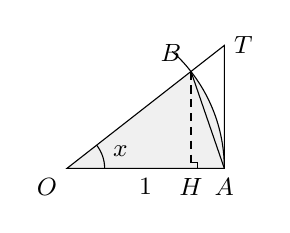
\begin{tikzpicture}[scale=2.0, font=\small]
\coordinate (O) at (0,0);
\coordinate (A) at (1,0);
\coordinate (B) at ({cos(38)},{sin(38)});
\coordinate (T) at (1,{tan(38)});
\coordinate (H) at ({cos(38)},0);
\fill[gray!12] (O)--(A) arc[start angle=0,end angle=38,radius=1]--cycle;
\draw (O)--(A)--(T)--cycle;
\draw (A)--(B);
\draw[densely dashed] (B)--(H);
\draw (H) ++(0,0.04)--++(0.04,0)--++(0,-0.04);
\draw (A) arc[start angle=0,end angle=48,radius=1];
\draw (0.24,0) arc[start angle=0,end angle=38,radius=0.24];
\node at (0.34,0.11) {$x$};
\node[below left] at (O) {$O$};
\node[below] at (A) {$A$};
\node[below] at (H) {$H$};
\node[above left] at (B) {$B$};
\node[right] at (T) {$T$};
\node[below] at (0.5,0) {$1$};
\end{tikzpicture}
\end{center}
作 $BH\perp OA$ 于 $H$, 则 $BH=\sin x$. 三个图形都以 $OA=1$ 为一边: $\triangle OAB$ 的底 $OA=1$, 高 $BH=\sin x$, 面积为 $\displaystyle\frac12\sin x$; 扇形 $OAB$ 的半径为 $1$, 圆心角为 $x$ 弧度, 面积为 $\displaystyle\frac12\cdot1^2\cdot x=\frac x2$; $\triangle OAT$ 的底 $OA=1$, 高 $AT=\tan x$, 面积为 $\displaystyle\frac12\tan x$. 由于弦 $AB$ 在圆内, $\triangle OAB$ 包含于扇形 $OAB$; 由于扇形内每一点的横坐标不超过 $1$, 扇形包含于 $\triangle OAT$. 两个包含关系都不是相等, 面积严格递增, 所以
\[
\frac12\sin x<\frac x2<\frac12\tan x,
\qquad\text{即}\quad \sin x<x<\tan x\quad\left(0<x<\frac\pi2\right).
\]
正弦是奇函数, 对 $\displaystyle-\frac\pi2<x<0$ 有 $|\sin x|=\sin(-x)<-x=|x|$; 当 $\displaystyle|x|\ge\frac\pi2$ 时 $|\sin x|\le1<|x|$. 所以对一切 $x$ 都有 $|\sin x|\le|x|$, 且 $x\ne0$ 时不等号严格.

由 $-|x|\le\sin x\le|x|$ 及 $\displaystyle\lim_{x\to0}|x|=0$, 两边夹定理给出 $\displaystyle\lim_{x\to0}\sin x=0$. 再由半角公式和复合函数极限 (令 $\displaystyle u=\frac x2$),
\[
\lim_{x\to0}(1-\cos x)
=\lim_{x\to0}2\sin^2\frac x2
=2\left(\lim_{u\to0}\sin u\right)^2=0,
\]
所以 $\displaystyle\lim_{x\to0}\cos x=1$.
\end{cnproof}
任意一点 $c$ 处的极限可由此得到. 令 $h=x-c$, 由和角公式及四则法则,
\[
\begin{aligned}
\lim_{x\to c}\sin x
&=\lim_{h\to0}(\sin c\cos h+\cos c\sin h)=\sin c\cdot1+\cos c\cdot0=\sin c,\\
\lim_{x\to c}\cos x
&=\lim_{h\to0}(\cos c\cos h-\sin c\sin h)=\cos c.
\end{aligned}
\]
\begin{theorem}[第一重要极限]
采用弧度制时, $\displaystyle \lim_{x\to0}\frac{\sin x}{x}=1$.
\end{theorem}
\par\indent\textbf{分析:} 由 $|\sin x|\le|x|$ 只知道比值的绝对值不超过 $1$, 还看不出它趋于 $1$. 面积比较同时给出了 $x<\tan x$, 改写为 $\displaystyle\frac{\sin x}x>\cos x$, 就得到一个趋于 $1$ 的下界, 可以夹逼.
\begin{cnproof}
对 $\displaystyle0<x<\frac\pi2$, 由 $\sin x<x<\tan x$ 及 $\sin x>0$, $\cos x>0$, 两边除以 $x$ 得 $\displaystyle\frac{\sin x}x<1$, 由 $\displaystyle x<\frac{\sin x}{\cos x}$ 得 $\displaystyle\cos x<\frac{\sin x}x$. 所以
\[
\cos x<\frac{\sin x}x<1\qquad\left(0<x<\frac\pi2\right).
\]
由 $\displaystyle\lim_{x\to0}\cos x=1$ 及两边夹定理, 右极限 $\displaystyle\lim_{x\to0^+}\frac{\sin x}x=1$. 比值 $\displaystyle\frac{\sin x}x$ 是偶函数, 左极限等于右极限, 故双侧极限为 $1$.
\end{cnproof}
\begin{example}
\textnormal{(教材例6.6)} 求 $\displaystyle \lim_{x\to0}\frac{1-\cos x}{2x^2}$.
\end{example}
\par\indent\textbf{分析:} 分子分母都趋于零, 要化成已知的 $\displaystyle\frac{\sin t}t$ 型. 分子中只有余弦, 半角公式 $1-\cos x=2\sin^2\frac x2$ 把它变成正弦的平方; 相应地分母要配成 $\displaystyle\left(\frac x2\right)^2$ 的倍数, 配分母时产生的常数系数必须保留.
\begin{cnproof}
\[
\begin{aligned}
\lim_{x\to0}\frac{1-\cos x}{2x^2}
&=\lim_{x\to0}\frac{2\sin^2\frac x2}{2x^2}
=\lim_{x\to0}\frac14\left(\frac{\sin\frac x2}{\frac x2}\right)^2\\
&=\frac14\left(\lim_{u\to0}\frac{\sin u}{u}\right)^2=\frac14,
\end{aligned}
\]
其中令 $\displaystyle u=\frac x2$, 用复合函数极限与乘积法则.
\end{cnproof}
由此得到以后常用的结果 $\displaystyle\lim_{x\to0}\frac{1-\cos x}{x^2}=\frac12$.
\begin{example}
\textnormal{(课堂例题: 第一重要极限的基本变形)} 求
\[
\text{(1)}\ \lim_{x\to0}\frac{x}{\sin x};\qquad
\text{(2)}\ \lim_{x\to\infty}x\sin\frac1x;\qquad
\text{(3)}\ \lim_{x\to0}\frac{\tan x}{x};\qquad
\text{(4)}\ \lim_{x\to0}\frac{\sin2x}{\tan5x}.
\]
\end{example}
\par\indent\textbf{分析:} 各题都要变形到 $\displaystyle\frac{\sin t}t$, 其中正弦的自变量与分母必须是同一个趋零的量. (1) 是基本极限的倒数, 分母极限为 $1\ne0$, 用商的法则. (2) 中趋零的量是 $\displaystyle\frac1x$, 令 $\displaystyle t=\frac1x$ 换元. (3) 把正切拆成正弦除以余弦. (4) 的两个角 $2x,5x$ 不同, 分别配成 $\displaystyle\frac{\sin2x}{2x}$ 与 $\displaystyle\frac{5x}{\sin5x}$, 补出的系数 $\displaystyle\frac{2x}{5x}=\frac25$ 保留下来.
\begin{cnproof}
(1) 由商的法则,
\[
\lim_{x\to0}\frac{x}{\sin x}=\frac1{\displaystyle\lim_{x\to0}\frac{\sin x}x}=1.
\]
(2) 令 $\displaystyle t=\frac1x$, 当 $x\to\infty$ 时 $t\to0$ 且 $t\ne0$, 由复合函数极限,
\[
\lim_{x\to\infty}x\sin\frac1x=\lim_{t\to0}\frac{\sin t}t=1;
\]
正、负无穷两个方向都成立.
(3) 由 $\displaystyle\lim_{x\to0}\cos x=1\ne0$,
\[
\lim_{x\to0}\frac{\tan x}x=\lim_{x\to0}\left(\frac{\sin x}x\cdot\frac1{\cos x}\right)=1\cdot\frac11=1.
\]
(4) 在 $0$ 的去心邻域内 $\tan5x\ne0$, 并令 $u=2x$, $v=5x$,
\[
\begin{aligned}
\lim_{x\to0}\frac{\sin2x}{\tan5x}
&=\lim_{x\to0}\left(\frac25\cdot\frac{\sin2x}{2x}\cdot\frac{5x}{\sin5x}\cdot\cos5x\right)\\
&=\frac25\cdot\lim_{u\to0}\frac{\sin u}u\cdot\frac1{\displaystyle\lim_{v\to0}\frac{\sin v}v}\cdot\lim_{x\to0}\cos5x
=\frac25\cdot1\cdot1\cdot1=\frac25.
\end{aligned}
\]
\end{cnproof}
\begin{example}
\textnormal{(课堂例题: 反三角函数的换元)} 求 $\displaystyle\lim_{x\to0}\frac{\arcsin x}{x}$ 及 $\displaystyle\lim_{x\to0}\frac{\arctan x}{x}$.
\end{example}
\par\indent\textbf{分析:} 已知的是三角函数的极限, 题目中出现的是反三角函数. 把反三角函数的值记为新变量 $t$, 原自变量就成为 $x=\sin t$ 或 $x=\tan t$, 式子回到上一例的形式. 换元要用复合函数极限定理, 须先验证 $x\to0$ 时 $t\to0$, 且 $x\ne0$ 时 $t\ne0$; 前者由反三角函数的单调性反解.
\begin{cnproof}
令 $t=\arcsin x$ ($-1\le x\le1$), 则 $x=\sin t$, $\displaystyle-\frac\pi2\le t\le\frac\pi2$. 先证 $x\to0$ 时 $t\to0$: 任给 $\varepsilon>0$, 令 $\displaystyle\eta=\min\left\{\varepsilon,\frac\pi4\right\}$, 取 $\delta=\sin\eta>0$; 当 $0<|x|<\delta$ 时, 由反正弦在 $[-1,1]$ 上严格递增, $|t|<\eta\le\varepsilon$. 又 $x\ne0$ 时 $t\ne0$. 由复合函数极限,
\[
\lim_{x\to0}\frac{\arcsin x}x=\lim_{t\to0}\frac t{\sin t}=1.
\]
同理令 $t=\arctan x$, 则 $x=\tan t$; 对上述 $\eta$, 当 $|x|<\tan\eta$ 时 $|t|<\eta\le\varepsilon$, 故 $t\to0$, 且 $x\ne0$ 时 $t\ne0$. 于是
\[
\lim_{x\to0}\frac{\arctan x}x=\lim_{t\to0}\frac t{\tan t}=1.
\]
\end{cnproof}
\begin{theorem}[第二重要极限]
\[
\lim_{x\to\infty}\left(1+\frac1x\right)^x=e,
\qquad
\lim_{t\to0}(1+t)^{\frac1t}=e.
\]
\end{theorem}
\par\indent\textbf{分析:} 1.4 已证明整数下标的 $\displaystyle\left(1+\frac1n\right)^n\to e$, 现在 $x$ 是实数, 不能直接代入. 要把实数 $x$ 与整数联系起来, 用相邻整数 $n=[x]$ 与 $n+1$ 夹住它: $n\le x<n+1$. 由此 $\displaystyle\frac1{n+1}<\frac1x\le\frac1n$, 底数被夹在 $\displaystyle1+\frac1{n+1}$ 与 $\displaystyle1+\frac1n$ 之间; 当 $x\to+\infty$ 时这些底数都大于 $1$, 底数越大、指数越大则幂越大, 于是幂被夹在 $\displaystyle\left(1+\frac1{n+1}\right)^n$ 与 $\displaystyle\left(1+\frac1n\right)^{n+1}$ 之间. 两端稍加改写就是已知数列的乘积或商, 都趋于 $e$.

$x\to-\infty$ 时底数小于 $1$, 上面关于幂的单调性不再适用. 令 $y=-x\to+\infty$, 把 $\displaystyle\left(1-\frac1y\right)^{-y}$ 的底数取倒数, 得 $\displaystyle\frac y{y-1}=1+\frac1{y-1}$, 转回正无穷处已证的形式.
\begin{cnproof}
先设 $x\to+\infty$, 只需考虑 $x\ge1$. 令 $n=[x]$, 则 $n\ge1$, $n\le x<n+1$, 从而 $\displaystyle1+\frac1{n+1}<1+\frac1x\le1+\frac1n$. 三个底数都大于 $1$, 幂关于底数和指数都递增, 所以
\[
\left(1+\frac1{n+1}\right)^n
\le\left(1+\frac1x\right)^x
\le\left(1+\frac1n\right)^{n+1}.
\]
两端分别等于
\[
\frac{\left(1+\frac1{n+1}\right)^{n+1}}{1+\frac1{n+1}},\qquad
\left(1+\frac1n\right)^n\left(1+\frac1n\right),
\]
当 $n\to\infty$ 时由 1.4 的结论及四则法则都趋于 $e$. 当 $x\to+\infty$ 时 $n=[x]\to+\infty$ (对任意 $N$, $x>N+1$ 时 $n>N$), 所以两端作为 $x$ 的函数也趋于 $e$. 由两边夹定理, $\displaystyle\lim_{x\to+\infty}\left(1+\frac1x\right)^x=e$.

再设 $x\to-\infty$, 令 $y=-x\to+\infty$, 只需考虑 $y>1$. 则
\[
\left(1+\frac1x\right)^x=\left(1-\frac1y\right)^{-y}
=\left(\frac{y}{y-1}\right)^{y}
=\left(1+\frac1{y-1}\right)^{y-1}\left(1+\frac1{y-1}\right).
\]
令 $u=y-1\to+\infty$, 由已证的正无穷情形及乘积法则,
\[
\lim_{x\to-\infty}\left(1+\frac1x\right)^x
=\lim_{u\to+\infty}\left(1+\frac1u\right)^u\cdot\lim_{u\to+\infty}\left(1+\frac1u\right)=e\cdot1=e.
\]
两个方向的极限相同, 故 $\displaystyle\lim_{x\to\infty}\left(1+\frac1x\right)^x=e$. 最后令 $\displaystyle x=\frac1t$: 当 $t\to0^+$ 时 $x\to+\infty$, $t\to0^-$ 时 $x\to-\infty$, 由复合函数极限得第二个等式.
\end{cnproof}
\begin{propositionsingle}[幂指表达式的有限极限]
若 $u(x)\to A$, $v(x)\to B$, 且 $B>0$, 则 $v(x)^{u(x)}\to B^A$.
\end{propositionsingle}
\begin{cnproof}
以 $x\to a$ 为例. 由保号性, $v(x)$ 在某个去心邻域内为正, 可写 $v^u=e^{u\ln v}$. 由 1.5 中 $\ln x\to\ln x_0$ 的结论及复合函数极限, $\ln v(x)\to\ln B$; 由乘积法则 $u\ln v\to A\ln B$; 再由 $e^x$ 在任意点的极限 (教材例6.3) 及复合函数极限,
\[
\lim_{x\to a}v(x)^{u(x)}=\lim_{x\to a}e^{u(x)\ln v(x)}=e^{A\ln B}=B^A.
\]
其他趋近方式同理.
\end{cnproof}
命题要求指数有有限极限、底数极限为正. 若底数趋于 $1$ 而指数无界 (“$1^\infty$”型), 底数与指数不能分别取极限, 结果取决于两者趋近的相对速度; 第二重要极限 $\displaystyle(1+t)^{\frac1t}\to e$ 就是这种情形的基本例子.
\par\indent\textbf{幂指极限的转化.} 对 $(1+u)^v$ 型的极限, 其中 $u\to0$ 而 $v$ 无界, 第二重要极限提供的可用整体是 $\displaystyle(1+u)^{\frac1u}$. 为了用上它, 把原指数 $v$ 写成 $\displaystyle\frac1u$ 的倍数, 这个倍数只能是 $uv$:
\[
(1+u)^v=\left[(1+u)^{\frac1u}\right]^{uv}.
\]
右边方括号内趋于 $e$. 若 $uv\to c$ (有限), 由上面的命题, 整个式子趋于 $e^c$; 以 $x\to a$ 为例,
\[
\lim_{x\to a}(1+u)^v=\left(\lim_{x\to a}(1+u)^{\frac1u}\right)^{\lim\limits_{x\to a}uv}=e^{c}.
\]
使用时须验证: $u$ 在所考察范围内非零, 底数 $1+u$ 为正, 且 $uv$ 有有限极限. 若 $uv$ 没有极限, 这条办法不能下结论. 取对数也是常用做法, 但 $\ln(1+u)\sim u$ 要到 1.8 才建立, 本节先用上述恒等改写.
\begin{example}
\textnormal{(教材例6.7)} 求 $\displaystyle \lim_{x\to\infty}\left(\frac{2x+1}{2x+3}\right)^x$.
\end{example}
\par\indent\textbf{分析:} 底数趋于 $1$, 指数趋于无穷, 是 $1^\infty$ 型. 按上面的转化, 先把底数写成 $1+t$: 分子与分母相差 $-2$, 所以 $\displaystyle t=\frac{2x+1}{2x+3}-1=-\frac2{2x+3}$. 再算 $t$ 与原指数 $x$ 的乘积 $\displaystyle xt=-\frac{2x}{2x+3}$, 它趋于 $-1$. 两件事都成立, 结果就是 $e^{-1}$.
\begin{cnproof}
令 $\displaystyle t=-\frac2{2x+3}$, 当 $x\to\infty$ 时 $t\to0$, 且 $t\ne0$, 底数 $1+t>0$ (当 $|x|$ 足够大时). 于是
\[
\left(\frac{2x+1}{2x+3}\right)^x=\left[(1+t)^{\frac1t}\right]^{xt},
\qquad
\lim_{x\to\infty}xt=\lim_{x\to\infty}\frac{-2x}{2x+3}=\lim_{x\to\infty}\frac{-2}{2+\frac3x}=-1.
\]
由第二重要极限 (复合函数极限) 及幂指表达式的有限极限命题,
\[
\lim_{x\to\infty}\left(\frac{2x+1}{2x+3}\right)^x
=\left(\lim_{x\to\infty}(1+t)^{\frac1t}\right)^{\lim\limits_{x\to\infty}xt}=e^{-1}.
\]
这一计算对正、负无穷两个方向同时有效.
\end{cnproof}
\begin{example}
\textnormal{(教材例6.8)} 证明 $\displaystyle \lim_{x\to a}x^\mu=a^\mu$, 其中 $a>0$, $\mu\in\mathbb R$.
\end{example}
\par\indent\textbf{分析:} $\mu$ 是正整数时, 教材例5.2 已用幂差公式证明. 一般实数 $\mu$ 不能作有限次乘法, 实数幂的定义本身依赖指数与对数: $x^\mu=e^{\mu\ln x}$. 于是问题化为已证的两个极限 $\ln x\to\ln a$ 和 $e^u\to e^{u_0}$ 的复合. 条件 $a>0$ 保证 $a$ 附近的 $x$ 为正, 对数有意义.
\begin{cnproof}
由 $a>0$, 在 $a$ 的某个邻域内 $x>0$, 可写 $x^\mu=e^{\mu\ln x}$. 由 1.5 的结论 $\ln x\to\ln a$ 及常数倍法则, $u=\mu\ln x\to\mu\ln a$; 再由 $e^u$ 在点 $\mu\ln a$ 处的极限 (教材例6.3) 及复合函数极限,
\[
\lim_{x\to a}x^\mu=\lim_{x\to a}e^{\mu\ln x}=e^{\mu\ln a}=a^\mu.
\]
\end{cnproof}

\subsection{指定作业: 运算与重要极限的应用}
以下题目练习三类转化: 约去使分子分母同时趋于零的公因子, 把三角式化为同角的 $\displaystyle\frac{\sin t}t$, 把 $1^\infty$ 型幂指式化为第二重要极限. 每题先看清趋近方式与定义域, 再决定变形.
\begin{example}
\textnormal{(指定作业: 习题1.6第1题(4))} 求 $\displaystyle \lim_{x\to\infty}\frac{x^2-1}{2x^2-x-1}$.
\end{example}
\par\indent\textbf{分析:} 分子分母都趋于无穷, 同除以最高次幂 $x^2$ 后各项都有有限极限, 与数列的有理式极限相同.
\begin{cnproof}
对 $x\ne0$, 分子分母同除以 $x^2$,
\[
\lim_{x\to\infty}\frac{x^2-1}{2x^2-x-1}
=\lim_{x\to\infty}\frac{1-\frac1{x^2}}{2-\frac1x-\frac1{x^2}}
=\frac{1-0}{2-0-0}=\frac12.
\]
分母极限为 $2\ne0$, 商的法则可用.
\end{cnproof}
\begin{example}
\textnormal{(指定作业: 习题1.6第1题(5))} 求 $\displaystyle \lim_{x\to1}\left(\frac1{1-x}-\frac3{1-x^3}\right)$.
\end{example}
\par\indent\textbf{分析:} 与教材例6.2 同型: 两个分式各自无有限极限, 通分后看相减剩下什么. $1-x^3=(1-x)(1+x+x^2)$, 通分后分子 $x^2+x-2=(x-1)(x+2)$ 在 $x=1$ 处为零, 可与分母约去一个因子; 约分时注意 $1-x=-(x-1)$ 带来的负号.
\begin{cnproof}
在 $x\ne1$ 时,
\[
\begin{aligned}
\lim_{x\to1}\left(\frac1{1-x}-\frac3{1-x^3}\right)
&=\lim_{x\to1}\frac{(1+x+x^2)-3}{(1-x)(1+x+x^2)}
=\lim_{x\to1}\frac{(x-1)(x+2)}{-(x-1)(1+x+x^2)}\\
&=\lim_{x\to1}\frac{-(x+2)}{1+x+x^2}=\frac{-3}{3}=-1.
\end{aligned}
\]
\end{cnproof}
\begin{example}
\textnormal{(指定作业: 习题1.6第1题(6))} 求 $\displaystyle \lim_{x\to4}\frac{\sqrt{2x+1}-3}{\sqrt{x-2}-\sqrt2}$.
\end{example}
\par\indent\textbf{分析:} 代入 $x=4$ 时分子、分母都为零, 需要比较两者趋于零的速度. 根式差本身看不出含有因子 $x-4$, 各乘以共轭式后, 分子变为 $2x+1-9=2(x-4)$, 分母变为 $x-2-2=x-4$, 公因子显露出来, 约去后余下的因子在 $x=4$ 处均非零.
\begin{cnproof}
在 $4$ 的去心邻域内 ($x>2$, $x\ne4$),
\[
\begin{aligned}
\lim_{x\to4}\frac{\sqrt{2x+1}-3}{\sqrt{x-2}-\sqrt2}
&=\lim_{x\to4}\left[\frac{2(x-4)}{\sqrt{2x+1}+3}\cdot\frac{\sqrt{x-2}+\sqrt2}{x-4}\right]\\
&=\lim_{x\to4}\frac{2\left(\sqrt{x-2}+\sqrt2\right)}{\sqrt{2x+1}+3}
=\frac{2\cdot2\sqrt2}{3+3}=\frac{2\sqrt2}3.
\end{aligned}
\]
根式的极限由本节根式极限例题得到.
\end{cnproof}
\begin{example}
\textnormal{(指定作业: 习题1.6第2题(4))} 求 $\displaystyle \lim_{x\to a}\frac{\sin x-\sin a}{x-a}$.
\end{example}
\par\indent\textbf{分析:} 分子是两个正弦之差, 分母是自变量之差, 两者都趋于零. 和差化积把分子变成乘积 $\displaystyle2\cos\frac{x+a}2\sin\frac{x-a}2$, 其中正弦的自变量 $\displaystyle\frac{x-a}2$ 与分母只差常数倍, 配成 $\displaystyle\frac{\sin\frac{x-a}2}{\frac{x-a}2}$ 即可; 余弦因子趋于 $\cos a$.
\begin{cnproof}
由和差化积, 令 $\displaystyle u=\frac{x-a}2\to0$ ($u\ne0$),
\[
\begin{aligned}
\lim_{x\to a}\frac{\sin x-\sin a}{x-a}
&=\lim_{x\to a}\left(\cos\frac{x+a}2\cdot\frac{\sin\frac{x-a}2}{\frac{x-a}2}\right)\\
&=\lim_{x\to a}\cos\frac{x+a}2\cdot\lim_{u\to0}\frac{\sin u}u=\cos a\cdot1=\cos a.
\end{aligned}
\]
余弦因子的极限用本节已证的任意点处三角函数极限.
\end{cnproof}
\begin{example}
\textnormal{(指定作业: 习题1.6第2题(6))} 求 $\displaystyle \lim_{x\to0}\frac{\tan x-\sin x}{\sin^3x}$.
\end{example}
\par\indent\textbf{分析:} 分子的两项都趋于零, 且都与 $x$ 很接近, 相减后剩下的量比 $x$ 小得多; 分母 $\sin^3x$ 也很小, 不能把分子、分母分别估计. 把正切写成 $\displaystyle\frac{\sin x}{\cos x}$ 后通分, 分子精确地化为 $\displaystyle\frac{\sin x(1-\cos x)}{\cos x}$, 与分母约去 $\sin x$ 后, 余下的 $\displaystyle\frac{1-\cos x}{\sin^2x}$ 可用 $\sin^2x=(1-\cos x)(1+\cos x)$ 再约分.
\begin{cnproof}
在 $0$ 的充分小去心邻域内 $\sin x\ne0$, $\cos x\ne0$,
\[
\begin{aligned}
\lim_{x\to0}\frac{\tan x-\sin x}{\sin^3x}
&=\lim_{x\to0}\frac{\sin x(1-\cos x)}{\cos x\sin^3x}
=\lim_{x\to0}\frac{1-\cos x}{\cos x\sin^2x}\\
&=\lim_{x\to0}\frac{1-\cos x}{\cos x(1-\cos x)(1+\cos x)}
=\lim_{x\to0}\frac1{\cos x(1+\cos x)}=\frac1{1\cdot2}=\frac12.
\end{aligned}
\]
\end{cnproof}
\begin{example}
\textnormal{(指定作业: 习题1.6第2题(8))} 求 $\displaystyle \lim_{x\to0}\frac{\sqrt{1-\cos x}}x$.
\end{example}
\par\indent\textbf{分析:} 由半角公式 $1-\cos x=2\sin^2\frac x2$, 开方得 $\displaystyle\sqrt2\left|\sin\frac x2\right|$, 带有绝对值; 分母 $x$ 则保留符号. 因此应分左右两侧: $x>0$ 时去掉绝对值不变号, $x<0$ 时要添负号. 两侧极限不同, 双侧极限不存在.
\begin{cnproof}
对 $x\ne0$,
\[
\frac{\sqrt{1-\cos x}}x
=\frac{\sqrt2\left|\sin\frac x2\right|}{x}.
\]
当 $x>0$ 时, $\displaystyle0<\frac x2<\frac\pi2$ (限制 $0<x<\pi$) 内 $\displaystyle\sin\frac x2>0$, 故
\[
\lim_{x\to0^+}\frac{\sqrt{1-\cos x}}x
=\lim_{x\to0^+}\frac{\sqrt2\sin\frac x2}{x}
=\frac{\sqrt2}2\lim_{x\to0^+}\frac{\sin\frac x2}{\frac x2}=\frac{\sqrt2}2.
\]
当 $x<0$ 时, $\displaystyle\left|\sin\frac x2\right|=-\sin\frac x2$, 同理左极限为 $\displaystyle-\frac{\sqrt2}2$. 两侧极限不相等, 故所求极限不存在.
\end{cnproof}
\begin{example}
\textnormal{(指定作业: 习题1.6第2题(10))} 求 $\displaystyle \lim_{x\to0}(1-\tan x)^{\frac1{\sin x}}$.
\end{example}
\par\indent\textbf{分析:} 底数趋于 $1$, 指数趋于无穷, 用幂指极限的转化. 底数减 $1$ 得 $t=-\tan x$; 它与原指数的乘积为 $\displaystyle-\frac{\tan x}{\sin x}=-\frac1{\cos x}$, 趋于 $-1$.
\begin{cnproof}
令 $t=-\tan x$, 当 $x\to0$ 时 $t\to0$, 在 $0$ 的充分小去心邻域内 $t\ne0$ 且 $1+t>0$. 于是
\[
(1-\tan x)^{\frac1{\sin x}}=\left[(1+t)^{\frac1t}\right]^{\frac{t}{\sin x}},
\qquad
\lim_{x\to0}\frac{t}{\sin x}=\lim_{x\to0}\frac{-\tan x}{\sin x}=\lim_{x\to0}\frac{-1}{\cos x}=-1.
\]
由第二重要极限及幂指表达式的有限极限命题,
\[
\lim_{x\to0}(1-\tan x)^{\frac1{\sin x}}=e^{-1}.
\]
\end{cnproof}
\begin{example}
\textnormal{(指定作业: 习题1.6第2题(11))} 求 $\displaystyle \lim_{x\to\infty}\left(\frac{2x-1}{2x+1}\right)^x$.
\end{example}
\par\indent\textbf{分析:} 与教材例6.7 同型, 底数写成 $\displaystyle1-\frac2{2x+1}$, 增量与原指数的乘积 $\displaystyle-\frac{2x}{2x+1}$ 在两个无穷方向都趋于 $-1$.
\begin{cnproof}
令 $\displaystyle t=-\frac2{2x+1}$, 当 $x\to\infty$ 时 $t\to0$, 且 $|x|$ 足够大时 $t\ne0$, $1+t>0$. 由
\[
\lim_{x\to\infty}xt=\lim_{x\to\infty}\frac{-2x}{2x+1}=\lim_{x\to\infty}\frac{-2}{2+\frac1x}=-1,
\]
得
\[
\lim_{x\to\infty}\left(\frac{2x-1}{2x+1}\right)^x
=\lim_{x\to\infty}\left[(1+t)^{\frac1t}\right]^{xt}=e^{-1}.
\]
\end{cnproof}
\begin{example}
\textnormal{(指定作业: 习题1.6第2题(13))} 对固定的实数 $x$, 求 $\displaystyle \lim_{n\to\infty}\left(1+\frac xn+\frac{x^2}{2n^2}\right)^{-n}$.
\end{example}
\par\indent\textbf{分析:} 这里趋于无穷的是 $n$, $x$ 是固定参数. 底数趋于 $1$, 指数 $-n$ 无界, 仍用幂指极限的转化: 把底数偏离 $1$ 的全部部分记为 $\displaystyle t_n=\frac xn+\frac{x^2}{2n^2}$, 再算 $-nt_n$. 二次小项 $\displaystyle\frac{x^2}{2n^2}$ 乘以 $n$ 后仍趋于零, 对结果没有贡献, 但在恒等变形完成前不能删去. 当 $x=0$ 时 $t_n=0$, 不能写 $\displaystyle\frac1{t_n}$, 单独处理.
\begin{cnproof}
若 $x=0$, 数列恒为 $1$, 极限为 $1=e^{0}$. 若 $x\ne0$, 令 $\displaystyle t_n=\frac xn+\frac{x^2}{2n^2}$, 则 $t_n\to0$, 充分大的 $n$ 有 $t_n\ne0$, 且底数 $\displaystyle1+t_n=\frac12\left[\left(1+\frac xn\right)^2+1\right]>0$. 于是
\[
\left(1+t_n\right)^{-n}=\left[(1+t_n)^{\frac1{t_n}}\right]^{-nt_n},
\qquad
\lim_{n\to\infty}(-nt_n)=\lim_{n\to\infty}\left(-x-\frac{x^2}{2n}\right)=-x.
\]
由第二重要极限与海涅定理, $(1+t_n)^{\frac1{t_n}}\to e$; 再由幂指表达式的有限极限 (数列情形),
\[
\lim_{n\to\infty}\left(1+\frac xn+\frac{x^2}{2n^2}\right)^{-n}=e^{-x}.
\]
\end{cnproof}
\begin{example}
\textnormal{(指定作业: 习题1.6第2题(14))} 求 $\displaystyle \lim_{x\to0}(\cos x)^{\frac1{x^2}}$.
\end{example}
\par\indent\textbf{分析:} 底数趋于 $1$, 指数趋于无穷. 增量 $t=\cos x-1$ 与指数的乘积为 $\displaystyle\frac{\cos x-1}{x^2}$, 由教材例6.6 后的结果它趋于 $\displaystyle-\frac12$. 底数趋于 $1$ 本身不能决定结果, 决定结果的是增量与指数乘积的极限.
\begin{cnproof}
令 $t=\cos x-1$, 当 $x\to0$ 时 $t\to0$, 且在 $0$ 的充分小去心邻域内 $t\ne0$, $1+t=\cos x>0$. 由
\[
\lim_{x\to0}\frac t{x^2}=\lim_{x\to0}\frac{-(1-\cos x)}{x^2}=-\frac12,
\]
得
\[
\lim_{x\to0}(\cos x)^{\frac1{x^2}}
=\lim_{x\to0}\left[(1+t)^{\frac1t}\right]^{\frac t{x^2}}=e^{-\frac12}.
\]
\end{cnproof}
\begin{example}
\textnormal{(指定作业: 习题1.6第6题)} 已知 $\displaystyle \lim_{x\to\infty}\left(\frac{x+a}{x-a}\right)^x=9$, 求常数 $a$.
\end{example}
\par\indent\textbf{分析:} 先把含参数 $a$ 的极限算出来, 再令它等于 $9$. 底数减 $1$ 得 $\displaystyle t=\frac{2a}{x-a}$, 与指数的乘积 $\displaystyle\frac{2ax}{x-a}\to2a$, 极限为 $e^{2a}$. 当 $a=0$ 时 $t=0$, 转化中的 $\displaystyle\frac1t$ 无意义, 先直接检查.
\begin{cnproof}
若 $a=0$, 原式恒为 $1$, 极限为 $1\ne9$, 不合题意. 设 $a\ne0$, 令 $\displaystyle t=\frac{2a}{x-a}$, 当 $x\to\infty$ 时 $t\to0$, $|x|$ 足够大时 $t\ne0$ 且 $1+t>0$. 由
\[
\lim_{x\to\infty}xt=\lim_{x\to\infty}\frac{2ax}{x-a}=\lim_{x\to\infty}\frac{2a}{1-\frac ax}=2a,
\]
得
\[
\lim_{x\to\infty}\left(\frac{x+a}{x-a}\right)^x
=\lim_{x\to\infty}\left[(1+t)^{\frac1t}\right]^{xt}=e^{2a}.
\]
由 $e^{2a}=9$ 得 $2a=\ln9$, 即 $a=\ln3$.
\end{cnproof}

\section{无穷小和无穷大}
前面各节计算的是变量趋近的值. 本节进一步比较趋近的速度: 两个量都趋于零时, 一个可能比另一个快得多, 也可能大致同步. 这种比较通过商来进行, 它能识别表达式中起主要作用的部分, 是化简极限计算的基本工具. 所有比较都只在指定的极限过程中有意义.
\subsection{无穷小及其运算}
\begin{definition}
在指定的极限过程中, 以 $0$ 为极限的变量称为该过程中的\textbf{无穷小量}, 简称\textbf{无穷小}.
\end{definition}
无穷小是一类变量, 不是一个数: 非零常数无论多小都不是无穷小, 常数 $0$ 则符合定义. 同一表达式在不同过程中性质可能不同, 例如 $x$ 在 $x\to0$ 时是无穷小, 在 $x\to+\infty$ 时不是. 讨论无穷小时必须写明极限过程.
\begin{example}
\textnormal{(教材例7.1)} 说明 $(x-a)^2$、$\sin(x-a)$ 在 $x\to a$ 时, 以及 $\displaystyle \frac1x$、$\displaystyle \frac1{3x}$、$\displaystyle \frac{x^2+x+1}{x^3+2}$ 在 $x\to\infty$ 时都是无穷小.
\end{example}
\par\indent\textbf{分析:} 判断无穷小只需验证指定过程中的极限为零, 可以使用已有的极限结论和运算法则, 不必回到定义. 前四个式子直接由幂函数、正弦在零点的极限及 $\displaystyle\frac1x\to0$ 得到; 最后一个是无穷远处的多项式商, 分母次数高于分子, 同除以分母的最高次幂 $x^3$ 后分子趋于零.
\begin{cnproof}
令 $h=x-a\to0$, 则 $(x-a)^2=h^2\to0$, $\sin(x-a)=\sin h\to0$. 当 $x\to\infty$ 时 $\displaystyle\frac1x\to0$, $\displaystyle\frac1{3x}=\frac13\cdot\frac1x\to0$. 最后一个, 分子分母同除以 $x^3$,
\[
\lim_{x\to\infty}\frac{x^2+x+1}{x^3+2}
=\lim_{x\to\infty}\frac{\frac1x+\frac1{x^2}+\frac1{x^3}}{1+\frac2{x^3}}
=\frac{0}{1}=0.
\]
故五个量在各自的过程中都是无穷小.
\end{cnproof}
\begin{theoremsingle}
在同一极限过程中, $f(x)\to L$ 的充分必要条件是 $f(x)=L+\alpha(x)$, 其中 $\alpha(x)$ 是该过程中的无穷小.
\end{theoremsingle}
\begin{cnproof}
若 $f\to L$, 令 $\alpha=f-L$, 由差的法则 $\alpha\to L-L=0$. 反过来, 若 $f=L+\alpha$ 且 $\alpha\to0$, 由和的法则 $f\to L+0=L$.
\end{cnproof}
这个定理把“有极限”改写为“极限值加无穷小”, 误差项 $\alpha$ 的大小便可以进一步讨论.
\begin{proposition}
在同一极限过程中: 有限个无穷小的和仍是无穷小; 无穷小与局部有界变量的乘积是无穷小; 特别地, 有限个无穷小的乘积仍是无穷小.
\end{proposition}
\begin{cnproof}
有限个无穷小之和由和的法则得零. 设 $\alpha\to0$, 而 $\beta$ 在所考察的范围内满足 $|\beta|\le M$ ($M>0$). 任给 $\varepsilon>0$, 由 $\alpha\to0$, 在相应范围内 $\displaystyle|\alpha|<\frac\varepsilon M$, 于是 $|\alpha\beta|\le M|\alpha|<\varepsilon$, 故 $\alpha\beta\to0$. 无穷小本身有极限, 因而局部有界, 乘积结论随之得到.
\end{cnproof}
无穷多个无穷小之和没有统一结论, 项数随变量增多时尤其不能套用有限和的法则. 两个无穷小之商也没有统一结论: 当 $x\to0$ 时 $\displaystyle\frac{x^2}x\to0$, $\displaystyle\frac xx=1$, 而 $\displaystyle\frac x{x^2}=\frac1x$ 没有有限极限. 商的不同情形正是下面比较无穷小的出发点.
\subsection{无穷大及其与无穷小的联系}
\begin{definition}
以 $x\to a$ 为例. 若对任意 $M>0$, 都存在 $\delta>0$, 使 $0<|x-a|<\delta$ 时恒有 $|f(x)|>M$, 则称 $f(x)$ 当 $x\to a$ 时为\textbf{无穷大量}, 简称\textbf{无穷大}, 记作 $\displaystyle\lim_{x\to a}f(x)=\infty$ 或 $f(x)\to\infty$ $(x\to a)$. 若把条件 $|f(x)|>M$ 换为 $f(x)>M$ 或 $f(x)<-M$, 则分别称为\textbf{正无穷大}或\textbf{负无穷大}, 记作 $f(x)\to+\infty$ 或 $f(x)\to-\infty$. 对其他极限过程, 把去心邻域换为相应的趋近范围.
\end{definition}
记号 $\infty$ 不表示实数, $f(x)\to\infty$ 只是“绝对值最终超过任给的正数”的简写, 这种情形下极限并不存在. 定义要求趋近范围内的\textbf{每一点}都满足 $|f(x)|>M$; 若只能找到一些点使 $|f(x)|$ 任意大, 只说明函数无界, 不能说明它是无穷大, 后面的 $x\cos x$ 就是例子. 无穷大不要求最终同号: $\displaystyle\frac1x$ 在 $x\to0$ 时是无穷大, 但左侧为负, 右侧为正.
\begin{example}
\textnormal{(教材例7.2)} 用定义证明 $\displaystyle \lim_{x\to1}\frac{x+2}{x^2-1}=\infty$.
\end{example}
\par\indent\textbf{分析:} 按定义, 要对任意 $M>0$ 找到半径, 使去心邻域内 $\displaystyle\left|\frac{x+2}{x^2-1}\right|>M$. 分母趋于零, 但这还不够: 若分子也趋于零, 商未必无穷大. 把分母分解为 $(x-1)(x+1)$, 原式的绝对值写成
\[
\left|\frac{x+2}{x+1}\right|\cdot\frac1{|x-1|}.
\]
后一个因子在 $x\to1$ 时增大, 前一个因子趋于 $\displaystyle\frac32$, 不会接近零. 为了得到简单的下界, 先把 $x$ 限制在 $1$ 附近的固定邻域内: 当 $\displaystyle|x-1|<\frac12$ 时 $\displaystyle\frac{x+2}{x+1}=1+\frac1{x+1}>1$, 于是整个绝对值大于 $\displaystyle\frac1{|x-1|}$. 剩下的任务只是解 $\displaystyle\frac1{|x-1|}>M$, 即 $\displaystyle|x-1|<\frac1M$. 两个限制取较小的半径.
\begin{cnproof}
先限制 $\displaystyle0<|x-1|<\frac12$, 则 $\displaystyle\frac12<x<\frac32$, $x+1>0$, 且
\[
\frac{x+2}{x+1}=1+\frac1{x+1}>1,
\qquad
\left|\frac{x+2}{x^2-1}\right|=\frac{x+2}{x+1}\cdot\frac1{|x-1|}>\frac1{|x-1|}.
\]
任给 $M>0$, 取 $\displaystyle\delta=\min\left\{\frac12,\frac1M\right\}$. 当 $0<|x-1|<\delta$ 时, 上述估计成立, 且 $\displaystyle\frac1{|x-1|}>M$, 所以 $\displaystyle\left|\frac{x+2}{x^2-1}\right|>M$. 由定义, $\displaystyle\lim_{x\to1}\frac{x+2}{x^2-1}=\infty$.

在所限范围内因子 $\displaystyle\frac{x+2}{x+1}$ 为正, 原式的符号由 $x-1$ 决定: $x\to1^-$ 时趋于 $-\infty$, $x\to1^+$ 时趋于 $+\infty$. 所以双侧只能写 $\infty$, 不能写成 $+\infty$.
\end{cnproof}
\begin{proposition}
在同一极限过程中: 若 $\alpha\to0$ 且 $\alpha$ 在所考察范围内不为零, 则 $\displaystyle\frac1\alpha\to\infty$; 若 $f\to\infty$, 则 $\displaystyle\frac1f\to0$. 两个无穷大之积是无穷大; 无穷大与局部有界变量之和是无穷大.
\end{proposition}
\begin{cnproof}
倒数关系: 任给 $M>0$, 由 $\alpha\to0$, 在相应范围内 $\displaystyle0<|\alpha|<\frac1M$, 即 $\displaystyle\left|\frac1\alpha\right|>M$; 反过来, 任给 $\varepsilon>0$, 由 $f\to\infty$, 在相应范围内 $\displaystyle|f|>\frac1\varepsilon$, 即 $\displaystyle\left|\frac1f\right|<\varepsilon$. 乘积: 任给 $M>0$, 使两个因子的绝对值都大于 $\sqrt M$, 则积的绝对值大于 $M$. 和: 设 $|g|\le C$, 任给 $M>0$, 使 $|f|>M+C$, 由反三角不等式 $|f+g|\ge|f|-|g|>M$.
\end{cnproof}
无穷大与无穷大之和、无穷大与无穷小之积都没有统一结论. 例如 $x\to+\infty$ 时, $x$ 与 $-x$ 之和为 $0$; $\displaystyle x\cdot\frac1{x^2}\to0$, $\displaystyle x\cdot\frac1x=1$, $\displaystyle x\cdot\frac1{\sqrt x}=\sqrt x\to+\infty$. 这类情形要具体计算.
\subsection{无穷小的阶、等价与主部}
设 $x\to0$. $x$ 与 $x^2$ 都是无穷小, $x$ 与 $2x$ 也都是无穷小, 两对的差 $x-x^2$ 和 $x-2x$ 都趋于零, 所以“差趋于零”不能区分它们. 但 $x^2$ 比 $x$ 小得多: $x=0.01$ 时 $x^2=0.0001$, 只有 $x$ 的百分之一; 而 $2x$ 始终是 $x$ 的两倍. 要描述这种相对大小, 应以其中一个量为尺度, 看另一个量占它的多少, 即考察比值的极限. 这就是下面定义的来源.
\begin{definition}
设在同一极限过程中 $\alpha,\beta$ 都是无穷小, 且 $\beta$ 在所考察范围内不为零.

(1) 若 $\displaystyle\frac\alpha\beta\to k$, 其中 $k$ 是非零常数, 则称 $\alpha$ 与 $\beta$ 是\textbf{同阶无穷小}; 特别地, 若 $k=1$, 则称 $\alpha$ 与 $\beta$ 是\textbf{等价无穷小}, 记作 $\alpha\sim\beta$.

(2) 若 $\displaystyle\frac\alpha\beta\to0$, 则称 $\alpha$ 是比 $\beta$ \textbf{高阶的无穷小}, 记作 $\alpha=o(\beta)$.

(3) 若 $\displaystyle\left|\frac\alpha\beta\right|\to+\infty$, 则称 $\alpha$ 是比 $\beta$ \textbf{低阶的无穷小}.
\end{definition}
高阶表示 $\alpha$ 比尺度 $\beta$ 更快地趋于零, 如 $x^2=o(x)$ $(x\to0)$; 同阶表示两者的大小差一个固定的非零倍数, 如 $2x$ 与 $x$ 同阶但不等价; 等价表示倍数恰为 $1$. 若比值不满足上述任何一种情形 (例如比值振荡), 就不能归入其中任何一类. 记号 $o(\beta)$ 表示某个比 $\beta$ 高阶的无穷小, 不是一个确定的函数. 教材把同阶关系记作 $\alpha=O(\beta)$; 通常文献中的大 $O$ 还可表示更宽的“比值有界”关系, 本书在作同阶判断时直接写出比值的极限.
\begin{definition}
设 $x\to0^+$. 若存在 $\mu>0$ 和非零常数 $k$, 使 $\displaystyle\frac{\alpha(x)}{x^\mu}\to k$, 则称 $\alpha(x)$ 是关于 $x$ 的 \textbf{$\mu$ 阶无穷小}, 并称 $kx^\mu$ 为 $\alpha(x)$ 的\textbf{主部}. 对 $x\to0$ 的双侧过程, 若 $x^\mu$ 在 $x<0$ 时有定义 (例如 $\mu$ 为正整数), 定义相同.
\end{definition}
阶数衡量趋于零的快慢, 阶数越高衰减越快. 主部保留大小和符号: 主部为 $-2x^3$ 表示 $\displaystyle\frac{\alpha}{x^3}\to-2$. 由定义, $\alpha$ 的主部为 $kx^\mu$ 当且仅当 $\alpha\sim kx^\mu$.
\begin{proposition}
在同一极限过程中, 设各无穷小在所考察范围内不为零.

(1) $\alpha\sim\beta$ 的充分必要条件是 $\alpha=\beta+o(\beta)$.

(2) 等价关系有对称性和传递性: $\alpha\sim\beta$ 推出 $\beta\sim\alpha$; $\alpha\sim\beta$, $\beta\sim\gamma$ 推出 $\alpha\sim\gamma$.

(3) (等价替换) 若 $\alpha\sim\widetilde\alpha$, $\beta\sim\widetilde\beta$, 且 $\displaystyle\frac{\widetilde\alpha}{\widetilde\beta}$ 的极限存在 (有限或为 $\infty$), 则 $\displaystyle\frac\alpha\beta$ 的极限存在且相同.
\end{proposition}
\begin{cnproof}
(1) 以 $\beta$ 为尺度衡量差 $\alpha-\beta$:
\[
\frac{\alpha-\beta}{\beta}=\frac\alpha\beta-1,
\]
所以 $\displaystyle\frac\alpha\beta\to1$ 当且仅当 $\displaystyle\frac{\alpha-\beta}\beta\to0$, 即 $\alpha-\beta=o(\beta)$.

(2) 若 $\displaystyle\frac\alpha\beta\to1$, 由商的法则 $\displaystyle\frac\beta\alpha=\frac1{\alpha/\beta}\to1$. 若还有 $\displaystyle\frac\beta\gamma\to1$, 则 $\displaystyle\frac\alpha\gamma=\frac\alpha\beta\cdot\frac\beta\gamma\to1$.

(3) 把原商写成替换后的商乘以两个趋于 $1$ 的因子:
\[
\frac\alpha\beta
=\frac\alpha{\widetilde\alpha}\cdot
\frac{\widetilde\alpha}{\widetilde\beta}\cdot
\frac{\widetilde\beta}{\beta}.
\]
若 $\displaystyle\frac{\widetilde\alpha}{\widetilde\beta}\to c$ (有限), 由乘积法则 $\displaystyle\frac\alpha\beta\to1\cdot c\cdot1=c$. 若 $\displaystyle\frac{\widetilde\alpha}{\widetilde\beta}\to\infty$, 则两个趋于 $1$ 的因子最终绝对值大于 $\displaystyle\frac12$, 于是 $\displaystyle\left|\frac\alpha\beta\right|>\frac14\left|\frac{\widetilde\alpha}{\widetilde\beta}\right|\to+\infty$.
\end{cnproof}
等价替换定理只适用于乘积和商中的\textbf{因子}: 替换一个因子, 相当于乘以一个趋于 $1$ 的量, 不改变极限. 它不适用于和差中的项: 若两项的主部相抵消, 相减后余下的量比原来的尺度小, 原先可以忽略的误差便可能成为结果的主要部分. 例如 $\tan x\sim x$, $\sin x\sim x$ $(x\to0)$, 但 $\tan x-\sin x$ 并不等价于 $x-x=0$ (零不能作为等价量的尺度), 它实际上是三阶无穷小, 见下面的例题. 遇到和差, 应先作精确的恒等变形, 把差化成乘积或商, 再替换.
\begin{example}
\textnormal{(教材例7.3)} 求 $\displaystyle \lim_{x\to0}\frac{x(\tan x-\sin x)}{\sin(x^4)}$.
\end{example}
\par\indent\textbf{分析:} 分子中 $\tan x$ 与 $\sin x$ 都以 $x$ 为主部, 相减后主部抵消, 不能分别替换. 要看清差的大小, 把正切写成 $\displaystyle\frac{\sin x}{\cos x}$ 并通分:
\[
\tan x-\sin x=\frac{\sin x-\sin x\cos x}{\cos x}=\frac{\sin x(1-\cos x)}{\cos x}.
\]
差变成了乘积, 各因子 $\sin x$、$1-\cos x$、$\cos x$ 的极限或等价量都已知: $\sin x\sim x$, $1-\cos x\sim\frac{x^2}2$. 分母 $\sin(x^4)\sim x^4$. 这时按因子分别计算即可.
\begin{cnproof}
在 $0$ 的充分小去心邻域内 $\cos x\ne0$, $\sin(x^4)\ne0$. 由上面的恒等变形,
\[
\frac{x(\tan x-\sin x)}{\sin(x^4)}
=\frac{\sin x}{x}\cdot\frac{1-\cos x}{x^2}\cdot\frac1{\cos x}\cdot\frac{x^4}{\sin(x^4)},
\]
右边每个因子都有有限极限, 由乘积法则 (其中令 $u=x^4\to0$),
\[
\begin{aligned}
\lim_{x\to0}\frac{x(\tan x-\sin x)}{\sin(x^4)}
&=\lim_{x\to0}\frac{\sin x}x\cdot\lim_{x\to0}\frac{1-\cos x}{x^2}\cdot\lim_{x\to0}\frac1{\cos x}\cdot\lim_{u\to0}\frac{u}{\sin u}\\
&=1\cdot\frac12\cdot1\cdot1=\frac12.
\end{aligned}
\]
\end{cnproof}
\begin{example}
\textnormal{(教材例7.4)} 当 $x\to0$ 时, $\sqrt{1+x^2}-\sqrt{1-x^2}$ 是关于 $x$ 的几阶无穷小?
\end{example}
\par\indent\textbf{分析:} 两个根式都趋于 $1$, 各自的极限不能反映相减后剩下多少. 根式之差用共轭式有理化: $(\sqrt A-\sqrt B)(\sqrt A+\sqrt B)=A-B$, 分子精确地变为 $2x^2$, 分母趋于 $2$. 于是以 $x^2$ 为尺度, 比值的极限为 $1$, 非零, 所以恰为二阶. 判断阶时, 比值极限非零这一点不能省略: 若极限为零, 说明阶数更高.
\begin{cnproof}
对 $x\ne0$, $|x|<1$,
\[
\lim_{x\to0}\frac{\sqrt{1+x^2}-\sqrt{1-x^2}}{x^2}
=\lim_{x\to0}\frac{(1+x^2)-(1-x^2)}{x^2\left(\sqrt{1+x^2}+\sqrt{1-x^2}\right)}
=\lim_{x\to0}\frac2{\sqrt{1+x^2}+\sqrt{1-x^2}}=\frac2{1+1}=1.
\]
极限为非零常数, 故 $\sqrt{1+x^2}-\sqrt{1-x^2}$ 是二阶无穷小, 且与 $x^2$ 等价, 主部为 $x^2$.
\end{cnproof}
\begin{example}
\textnormal{(教材例7.5)} 当 $x\to+\infty$ 时, 求 $\displaystyle \frac1{x\sqrt{1+x^2}}$ 关于 $\displaystyle\frac1x$ 的主部, 并写成主部加余项的形式.
\end{example}
\par\indent\textbf{分析:} $x\to+\infty$ 时 $\sqrt{1+x^2}$ 与 $x$ 大小相当, 分母的尺度是 $x^2$, 猜测主部为 $\displaystyle\frac1{x^2}$. 猜测要用比值验证: 原式除以 $\displaystyle\frac1{x^2}$ 得 $\displaystyle\frac x{\sqrt{1+x^2}}$, 把根号内的 $x^2$ 提出时用到 $\sqrt{x^2}=|x|=x$ ($x>0$), 比值趋于 $1$.
\begin{cnproof}
对 $x>0$,
\[
\lim_{x\to+\infty}\frac{\frac1{x\sqrt{1+x^2}}}{\frac1{x^2}}
=\lim_{x\to+\infty}\frac{x}{\sqrt{1+x^2}}
=\lim_{x\to+\infty}\frac1{\sqrt{\frac1{x^2}+1}}=1.
\]
故主部为 $\displaystyle\frac1{x^2}$, 即关于 $\displaystyle\frac1x$ 的二阶无穷小, 并有
\[
\frac1{x\sqrt{1+x^2}}=\frac1{x^2}+o\!\left(\frac1{x^2}\right)\quad(x\to+\infty).
\]
当 $x\to-\infty$ 时原式为负, $\sqrt{x^2}=-x$, 比值趋于 $-1$, 主部应为 $\displaystyle-\frac1{x^2}$; 所以必须注明方向.
\end{cnproof}
\par\indent\textbf{无穷大的比较.} 无穷大同样用比值比较. 设 $F,G$ 是同一过程中的无穷大. 若 $\displaystyle\frac FG$ 趋于非零常数, 称 $F$ 与 $G$ 是\textbf{同阶无穷大}, 趋于 $1$ 时称\textbf{等价}; 若 $\displaystyle\frac FG\to0$, 称 $F$ 是比 $G$ 低阶的无穷大; 若 $\displaystyle\left|\frac FG\right|\to+\infty$, 称 $F$ 是比 $G$ 高阶的无穷大. 若 $\displaystyle\frac F{G^\mu}\to k\ne0$ ($\mu>0$), 则称 $F$ 是关于 $G$ 的 $\mu$ 阶无穷大, $kG^\mu$ 为主部, 此时 $F=kG^\mu+o(G^\mu)$. 这里 $o(G^\mu)$ 仍表示比值趋于零, 余项本身未必趋于零.
\begin{example}
\textnormal{(教材例7.6)} 当 $x\to1$ 时, 求 $\displaystyle \frac1{\sin\pi x}$ 关于 $\displaystyle \frac1{x-1}$ 的阶与主部.
\end{example}
\par\indent\textbf{分析:} 按定义算比值 $\displaystyle\frac{1/\sin\pi x}{1/(x-1)}=\frac{x-1}{\sin\pi x}$. 已知 $\sin t\sim t$ 的条件是 $t\to0$, 而这里 $\pi x\to\pi$, 不能直接用. 令 $h=x-1\to0$, 把趋近点平移到零: $\sin\pi x=\sin(\pi+\pi h)=-\sin\pi h$, 其中 $\pi h\to0$, 就能用第一重要极限. 负号来自诱导公式, 它决定主部的符号.
\begin{cnproof}
令 $h=x-1$, 当 $x\to1$ 时 $h\to0$, $h\ne0$, 且 $\sin\pi x=\sin(\pi+\pi h)=-\sin\pi h$. 于是 (令 $u=\pi h\to0$)
\[
\lim_{x\to1}\frac{\frac1{\sin\pi x}}{\frac1{x-1}}
=\lim_{x\to1}\frac{x-1}{\sin\pi x}
=\lim_{h\to0}\frac{h}{-\sin\pi h}
=-\frac1\pi\lim_{u\to0}\frac{u}{\sin u}=-\frac1\pi.
\]
比值的极限有限且非零, 故 $\displaystyle\frac1{\sin\pi x}$ 是关于 $\displaystyle\frac1{x-1}$ 的一阶无穷大, 主部为 $\displaystyle-\frac1{\pi(x-1)}$, 即
\[
\frac1{\sin\pi x}=-\frac1{\pi(x-1)}+o\!\left(\frac1{x-1}\right)\quad(x\to1).
\]
\end{cnproof}
\begin{example}
\textnormal{(教材例7.7)} 已知 $\displaystyle \lim_{x\to\infty}\left(\frac{x^2}{x+1}-ax-b\right)=0$, 求 $a,b$.
\end{example}
\par\indent\textbf{分析:} 题目要求原函数与直线 $ax+b$ 之差趋于零. 只找出与 $\displaystyle\frac{x^2}{x+1}$ 等价的一次项还不够: 等价只保证相对误差趋于零, 差本身可以趋于非零常数. 分子次数比分母高一次, 多项式除法能把 $\displaystyle\frac{x^2}{x+1}$ 精确地写成一次式加真分式, 真分式趋于零, 一次式就是所求的 $ax+b$. 另一种做法是依次确定: 先看差中的一次项系数, 若不为零, 差无界, 故 $a=1$; 再看常数项.
\begin{cnproof}
作多项式除法, $x^2=(x+1)(x-1)+1$, 故
\[
\frac{x^2}{x+1}=x-1+\frac1{x+1},
\qquad
\frac{x^2}{x+1}-ax-b=(1-a)x-(1+b)+\frac1{x+1}.
\]
当 $x\to\infty$ 时 $\displaystyle\frac1{x+1}\to0$. 若 $a\ne1$, 则 $(1-a)x$ 是无穷大, 与有界的其余两项之和仍是无穷大, 不可能趋于零, 故 $a=1$. 此时差为 $\displaystyle-(1+b)+\frac1{x+1}\to-(1+b)$, 由条件 $-(1+b)=0$, 即 $b=-1$. 代回验证: $\displaystyle\frac{x^2}{x+1}-x+1=\frac1{x+1}\to0$.
\end{cnproof}
\begin{example}
\textnormal{(选自教材习题1.7第6题)} 为什么不能把 $\displaystyle \frac{\tan x-\sin x}{x^3}$ 中的 $\tan x$ 与 $\sin x$ 都替换为 $x$?
\end{example}
\par\indent\textbf{分析:} 等价替换定理只允许替换乘积或商中的因子, 而这里 $\tan x$ 和 $\sin x$ 是和差中的项. 两项分别替换会得到 $\displaystyle\frac{x-x}{x^3}=0$, 但教材例7.3 的精确分解表明 $\tan x-\sin x$ 的大小是 $\displaystyle\frac{x^3}2$, 所以正确答案是 $\displaystyle\frac12$.
\begin{cnproof}
由教材例7.3 的分解 $\displaystyle\tan x-\sin x=\frac{\sin x(1-\cos x)}{\cos x}$,
\[
\lim_{x\to0}\frac{\tan x-\sin x}{x^3}
=\lim_{x\to0}\left(\frac{\sin x}x\cdot\frac{1-\cos x}{x^2}\cdot\frac1{\cos x}\right)=1\cdot\frac12\cdot1=\frac12,
\]
而不是分别替换所得的 $0$. 替换 $\tan x\sim x$ 时丢掉的误差 $\tan x-x$ 与 $x^3$ 同阶, 它在相减后成为主要部分, 这就是分别替换出错的原因.
\end{cnproof}
对多项式之商, $x\to0$ 时分子分母各取最低次项, $|x|\to\infty$ 时各取最高次项, 就是提取主部后的等价替换.
\begin{example}
\textnormal{(补充题型: 主部抵消与求参)} 求常数 $a$, 使 $\sqrt{1+x}-1-ax$ 在 $x\to0$ 时是关于 $x$ 的二阶无穷小, 并求主部.
\end{example}
\par\indent\textbf{分析:} 记 $R(x)=\sqrt{1+x}-1-ax$. 二阶要求 $\displaystyle\frac{R(x)}{x^2}$ 趋于非零常数, 直接计算这个比值要同时处理根式和参数, 不便. 先用一个较弱的必要条件: 若 $\displaystyle\frac{R(x)}{x^2}\to k$, 则 $\displaystyle\frac{R(x)}x=x\cdot\frac{R(x)}{x^2}\to0$. 比值 $\displaystyle\frac{R(x)}x$ 容易算 (根式部分有理化), 它的极限是 $\displaystyle\frac12-a$, 必须为零, 由此确定 $a$. 然后对这个 $a$ 计算 $\displaystyle\frac{R(x)}{x^2}$, 验证极限非零; 若为零, 说明阶数更高, 不合要求.
\begin{cnproof}
若 $R(x)$ 是二阶无穷小, 则 $\displaystyle\frac{R(x)}x\to0$. 而
\[
\lim_{x\to0}\frac{\sqrt{1+x}-1-ax}{x}
=\lim_{x\to0}\left(\frac{(1+x)-1}{x\left(\sqrt{1+x}+1\right)}-a\right)
=\lim_{x\to0}\left(\frac1{\sqrt{1+x}+1}-a\right)=\frac12-a,
\]
所以必须 $\displaystyle a=\frac12$. 此时
\[
\sqrt{1+x}-1-\frac x2
=\frac{x}{\sqrt{1+x}+1}-\frac x2
=\frac{x\left(2-\sqrt{1+x}-1\right)}{2\left(\sqrt{1+x}+1\right)}
=\frac{x\left(1-\sqrt{1+x}\right)}{2\left(\sqrt{1+x}+1\right)}
=-\frac{x^2}{2\left(\sqrt{1+x}+1\right)^2},
\]
最后一步用 $\displaystyle1-\sqrt{1+x}=-\frac{x}{1+\sqrt{1+x}}$. 于是
\[
\lim_{x\to0}\frac{\sqrt{1+x}-1-\frac x2}{x^2}
=\lim_{x\to0}\frac{-1}{2\left(\sqrt{1+x}+1\right)^2}=-\frac18\ne0.
\]
故当 $\displaystyle a=\frac12$ 时原式恰为二阶无穷小, 主部为 $\displaystyle-\frac{x^2}8$.
\end{cnproof}
\subsection{指定作业与典型题型}
\begin{example}
\textnormal{(指定作业: 习题1.7第3题)} 函数 $f(x)=x\cos x$ 在 $\mathbb R$ 上是否有界? 当 $x\to\infty$ 时是否为无穷大?
\end{example}
\par\indent\textbf{分析:} 无界只需找到一列点使函数值的绝对值任意大; 无穷大则要求远处的所有点函数值的绝对值都大. 余弦的波峰处 $|f(x)|=|x|$ 很大, 余弦的零点处 $f(x)=0$, 而两类点在任意远处都有. 分别写出这两列点就能回答两问.
\begin{cnproof}
取 $x_n=2n\pi$, 则 $f(x_n)=2n\pi\cos2n\pi=2n\pi\to+\infty$, 所以 $f$ 无界. 另一方面取 $\displaystyle y_n=\frac\pi2+n\pi$, 则 $y_n\to+\infty$ 且 $f(y_n)=0$. 对任意 $A>0$, 总有 $y_n>A$, 而 $|f(y_n)|=0$ 不大于任何正数 $M$, 所以 $f$ 不满足 $x\to\infty$ 时无穷大的定义. 故 $f$ 无界, 但不是无穷大.
\end{cnproof}
\begin{example}
\textnormal{(指定作业: 习题1.7第5题(2)(4))} 证明
\[
\frac{x+2}{x^4+3}=o\!\left(\frac1{x^2}\right)\quad(x\to\infty),
\qquad
\sqrt{x+1}-\sqrt x=O\!\left(\frac1{\sqrt x}\right)\quad(x\to+\infty).
\]
第二式按教师更正取 $x\to+\infty$; $O$ 沿用教材的同阶约定.
\end{example}
\par\indent\textbf{分析:} 阶的关系都通过比值验证: 把待比较的量除以标准量, 比值趋于零对应小 $o$, 趋于非零常数对应同阶. 第一式的比值是多项式之商, 同除以最高次幂; 第二式的根式差先有理化.
\begin{cnproof}
第一式:
\[
\lim_{x\to\infty}\frac{\frac{x+2}{x^4+3}}{\frac1{x^2}}
=\lim_{x\to\infty}\frac{x^3+2x^2}{x^4+3}
=\lim_{x\to\infty}\frac{\frac1x+\frac2{x^2}}{1+\frac3{x^4}}=0,
\]
故 $\displaystyle\frac{x+2}{x^4+3}=o\!\left(\frac1{x^2}\right)$. 第二式:
\[
\lim_{x\to+\infty}\frac{\sqrt{x+1}-\sqrt x}{\frac1{\sqrt x}}
=\lim_{x\to+\infty}\frac{\sqrt x}{\sqrt{x+1}+\sqrt x}
=\lim_{x\to+\infty}\frac1{\sqrt{1+\frac1x}+1}=\frac12,
\]
比值趋于非零常数, 两者同阶, 且 $\displaystyle\sqrt{x+1}-\sqrt x\sim\frac1{2\sqrt x}$.
\end{cnproof}
\begin{example}
\textnormal{(指定作业: 习题1.7第7题(4))} 当 $x\to0$ 时, 求 $\tan x-\sin x$ 关于 $x$ 的阶和主部; 并求 $\displaystyle\lim_{x\to0}\frac{\tan x-\sin x}{x^2}$, 与分母为 $x^3$ 的情形比较.
\end{example}
\par\indent\textbf{分析:} 教材例7.3 的分解已给出 $\displaystyle\frac{\tan x-\sin x}{x^3}\to\frac12$, 这同时确定了阶和主部. 分母换为 $x^2$ 时, 把比值写成 $\displaystyle x\cdot\frac{\tan x-\sin x}{x^3}$, 多出的因子 $x$ 使极限为零, 说明以 $x^2$ 为尺度时该量是高阶的.
\begin{cnproof}
由 $\displaystyle\lim_{x\to0}\frac{\tan x-\sin x}{x^3}=\frac12\ne0$, $\tan x-\sin x$ 是三阶无穷小, 主部为 $\displaystyle\frac{x^3}2$. 又
\[
\lim_{x\to0}\frac{\tan x-\sin x}{x^2}
=\lim_{x\to0}\left(x\cdot\frac{\tan x-\sin x}{x^3}\right)=0\cdot\frac12=0.
\]
分母为 $x^2$ 时极限为 $0$, 为 $x^3$ 时极限为 $\displaystyle\frac12$: 同一个三阶量, 与低一阶的尺度相比趋于零, 与同阶的尺度相比趋于非零常数.
\end{cnproof}
\begin{example}
\textnormal{(指定作业: 习题1.7第8题(4))} 求
\[
\lim_{x\to0^+}\frac{\sin(x^3)\tan x(1-\cos x)}{\sqrt{x+\sqrt[3]x}\,\sqrt[6]{x^5}\sin^5x}.
\]
\end{example}
\par\indent\textbf{分析:} 分子分母都是若干因子的乘积, 可以逐个因子用等价替换. 三角因子的等价量已知:
\[
\sin(x^3)\sim x^3,\qquad \tan x\sim x,\qquad 1-\cos x\sim\frac{x^2}2,\qquad \sin^5x\sim x^5.
\]
根式 $\sqrt{x+\sqrt[3]x}$ 中有和, 要先判断 $x$ 与 $\sqrt[3]x$ 哪个是主要部分: 两者之比 $\displaystyle\frac x{\sqrt[3]x}=x^{\frac23}\to0$, 所以 $\sqrt[3]x$ 为主, 提出它后 $x+\sqrt[3]x=x^{\frac13}\left(1+x^{\frac23}\right)$, 根式等价于 $x^{\frac16}$. 各因子的幂次与系数分别合并后约分.
\begin{cnproof}
对 $x>0$,
\[
\sqrt{x+\sqrt[3]x}=\sqrt{x^{\frac13}\left(1+x^{\frac23}\right)}=x^{\frac16}\sqrt{1+x^{\frac23}}\sim x^{\frac16},
\qquad
\sqrt[6]{x^5}=x^{\frac56}.
\]
分子各因子的等价量为 $x^3$、$x$、$\displaystyle\frac{x^2}2$, 分母各因子的等价量为 $x^{\frac16}$、$x^{\frac56}$、$x^5$. 由等价替换定理,
\[
\lim_{x\to0^+}\frac{\sin(x^3)\tan x(1-\cos x)}{\sqrt{x+\sqrt[3]x}\,\sqrt[6]{x^5}\sin^5x}
=\lim_{x\to0^+}\frac{x^3\cdot x\cdot\frac{x^2}2}{x^{\frac16}\cdot x^{\frac56}\cdot x^5}
=\lim_{x\to0^+}\frac{x^6}{2x^6}=\frac12.
\]
题中 $\sin(x^3)$ 指先取立方再取正弦.
\end{cnproof}

\section{连续函数}
函数极限只考察一点附近的函数值, 与该点本身的函数值无关. 若还要求附近的函数值趋于该点的实际函数值, 就得到连续性. 本节先区分这两个要求并给出间断点的分类, 再证明连续性在四则运算、复合和求反函数下保持, 由此得到初等函数的连续性, 最后利用连续性建立对数、指数与幂函数的基本极限.
\subsection{连续的定义与间断点}
\begin{definition}
设 $f$ 在 $x_0$ 的某个邻域内有定义. 若对任意 $\varepsilon>0$, 存在 $\delta>0$, 使 $|x-x_0|<\delta$ 时 $|f(x)-f(x_0)|<\varepsilon$, 则称 $f$ 在点 $x_0$ \textbf{连续}. 若 $f$ 在区间内每一点都连续, 则称 $f$ 为该区间上的\textbf{连续函数}.
\end{definition}
与极限的定义相比, 这里有两处改变: 候选值换成了函数值 $f(x_0)$, 邻域不再去心. 因此 $f$ 在 $x_0$ 连续等价于三个条件同时成立: $f(x_0)$ 有定义, $\displaystyle\lim_{x\to x_0}f(x)$ 存在, 且 $\displaystyle\lim_{x\to x_0}f(x)=f(x_0)$. 记 $\Delta x=x-x_0$, $\Delta y=f(x_0+\Delta x)-f(x_0)$, 连续也可表述为 $\Delta x\to0$ 时 $\Delta y\to0$: 自变量的微小改变只引起函数值的微小改变.

若 $\displaystyle\lim_{x\to x_0^-}f(x)=f(x_0)$, 称 $f$ 在 $x_0$ \textbf{左连续}; 若 $\displaystyle\lim_{x\to x_0^+}f(x)=f(x_0)$, 称 $f$ 在 $x_0$ \textbf{右连续}. $f$ 在 $x_0$ 连续当且仅当它在 $x_0$ 既左连续又右连续. 在闭区间 $[a,b]$ 上连续, 指在 $(a,b)$ 内每点连续, 在 $a$ 右连续, 在 $b$ 左连续; 全体这样的函数记为 $C[a,b]$. 端点处只考察区间内的趋近方向.
\begin{definition}
设 $f$ 在 $x_0$ 的某个去心邻域内有定义. 若 $f$ 在 $x_0$ 无定义, 或虽有定义但不连续, 则称 $x_0$ 为 $f$ 的\textbf{间断点}. 若左、右极限 $f(x_0^-)$, $f(x_0^+)$ 都存在 (有限), 称 $x_0$ 为\textbf{第一类间断点}; 其中若 $f(x_0^-)=f(x_0^+)$, 称为\textbf{可去间断点}, 若 $f(x_0^-)\ne f(x_0^+)$, 称为\textbf{跳跃间断点}. 若左、右极限至少有一个不存在, 称 $x_0$ 为\textbf{第二类间断点}; 其中若至少有一侧的极限为 $\infty$, 也称\textbf{无穷间断点}.
\end{definition}
分类的依据先是两侧极限, 再是中心值. 可去间断点处两侧极限有共同的有限值 $L$, 只是 $f(x_0)$ 无定义或 $f(x_0)\ne L$, 补充定义或改定义 $f(x_0)=L$ 后函数就在该点连续, “可去”即此意. 跳跃间断点和第二类间断点处, 改变中心值不能消除间断. 判断某点的类型时, 应先分别计算左、右极限, 再与中心值比较.
\begin{example}
\textnormal{(教材例8.1)} 讨论下列函数在 $x=0$ 处的连续性:
\[
f_1(x)=x^2,\quad
f_2(x)=\begin{cases}|x|,&x\ne0,\\2,&x=0,\end{cases}\quad
f_3(x)=\frac{\sin x}{x}\ (x\ne0),\quad
f_4(x)=\begin{cases}e^{\frac1x},&x\ne0,\\1,&x=0.\end{cases}
\]
\end{example}
\par\indent\textbf{分析:} 对每个函数依次检查: 中心值有无定义, 两侧极限是否存在且相等, 极限是否等于中心值. 四个函数分别对应连续、中心值取错、中心值缺失、两侧极限不一致四种情形.
\begin{cnproof}
$f_1$: $\displaystyle\lim_{x\to0}x^2=0=f_1(0)$, 连续.

$f_2$: $\displaystyle\lim_{x\to0}|x|=0$, 而 $f_2(0)=2\ne0$, 故 $0$ 是可去间断点; 改定义 $f_2(0)=0$ 后连续.

$f_3$: 在 $0$ 无定义, 但 $\displaystyle\lim_{x\to0}\frac{\sin x}x=1$, 故 $0$ 是可去间断点; 补充定义 $f_3(0)=1$ 后连续.

$f_4$: 当 $x\to0^-$ 时 $\displaystyle\frac1x\to-\infty$, $e^{\frac1x}\to0$, 左极限为 $0$; 当 $x\to0^+$ 时 $\displaystyle\frac1x\to+\infty$, $e^{\frac1x}\to+\infty$, 右极限不存在. 故 $0$ 是第二类间断点 (无穷间断点), 无论中心值取什么都不连续.
\end{cnproof}
取整函数 $[x]$ 在每个整数 $k$ 处左极限为 $k-1$, 右极限为 $k$, 是跳跃间断点, 跳跃为 $1$; 在非整数点处连续.
\begin{example}
\textnormal{(教材例8.2)} 设
\[
f(x)=\begin{cases}\frac{\sin x}{x},&x<0,\\a,&x=0,\\x\sin\frac1x+b,&x>0.\end{cases}
\]
问 $a,b$ 满足什么条件时 $\displaystyle\lim_{x\to0}f(x)$ 存在? 满足什么条件时 $f$ 在 $0$ 连续?
\end{example}
\par\indent\textbf{分析:} 分段点处左、右极限要按各自的表达式计算. 左侧是第一重要极限. 右侧的 $\displaystyle\sin\frac1x$ 没有极限, 但有界, 乘以趋零的 $x$ 后趋于零 (有界乘无穷小), 所以右极限为 $b$. 极限存在只要求两侧极限相等, 与中心值 $a$ 无关; 连续则还要求中心值等于这个极限.
\begin{cnproof}
左极限 $\displaystyle\lim_{x\to0^-}\frac{\sin x}x=1$. 右侧由 $\displaystyle\left|x\sin\frac1x\right|\le|x|\to0$ 及两边夹定理, $\displaystyle\lim_{x\to0^+}\left(x\sin\frac1x+b\right)=0+b=b$. 所以 $\displaystyle\lim_{x\to0}f(x)$ 存在当且仅当 $b=1$, 此时极限为 $1$, $a$ 可以任取. $f$ 在 $0$ 连续当且仅当极限存在且等于 $f(0)=a$, 即 $a=b=1$.
\end{cnproof}
\subsection{连续函数的运算与反函数}
\begin{theorem}
若 $f,g$ 都在 $x_0$ 连续, 则 $f\pm g$, $fg$ 在 $x_0$ 连续; 若还有 $g(x_0)\ne0$, 则 $\displaystyle\frac fg$ 在 $x_0$ 连续. 若 $g$ 在 $x_0$ 连续, $f$ 在 $u_0=g(x_0)$ 连续, 且复合函数 $f\circ g$ 在 $x_0$ 的某个邻域内有定义, 则 $f\circ g$ 在 $x_0$ 连续.
\end{theorem}
\par\indent\textbf{分析:} 四则部分把连续写成“极限等于函数值”, 再用极限的四则法则. 复合部分的目标是控制 $|f(g(x))-f(g(x_0))|$. $f$ 在 $u_0$ 连续说明: 输入 $u$ 离 $u_0$ 足够近时输出 $f(u)$ 离 $f(u_0)$ 足够近; 而 $g$ 在 $x_0$ 连续能使 $g(x)$ 离 $u_0$ 足够近. 因此先由目标误差 $\varepsilon$ 确定外层所需的输入误差 $\eta$, 再由 $\eta$ 确定内层的半径 $\delta$. 与复合函数的极限定理相比, 这里不必排除 $g(x)=u_0$, 因为外层在 $u_0$ 处的函数值本身就满足误差要求.
\begin{cnproof}
四则部分: 由 $\displaystyle\lim_{x\to x_0}f(x)=f(x_0)$, $\displaystyle\lim_{x\to x_0}g(x)=g(x_0)$ 及极限的四则法则, $\displaystyle\lim_{x\to x_0}[f(x)\pm g(x)]=f(x_0)\pm g(x_0)$, 乘积和商同理, 商的情形用到 $g(x_0)\ne0$.

复合部分: 任给 $\varepsilon>0$. 由 $f$ 在 $u_0$ 连续, 存在 $\eta>0$, 使 $|u-u_0|<\eta$ 时 $|f(u)-f(u_0)|<\varepsilon$. 由 $g$ 在 $x_0$ 连续, 存在 $\delta>0$, 使 $|x-x_0|<\delta$ 时 $|g(x)-u_0|<\eta$ (必要时缩小 $\delta$ 使复合有定义). 于是 $|x-x_0|<\delta$ 时, $u=g(x)$ 满足 $|u-u_0|<\eta$, 从而 $|f(g(x))-f(g(x_0))|<\varepsilon$.
\end{cnproof}
复合函数连续的结论可写成 $\displaystyle\lim_{x\to x_0}f(g(x))=f\left(\lim_{x\to x_0}g(x)\right)$: 对连续的外层函数, 极限号可以移到函数内部. 这是以后计算极限时最常用的工具之一.
\begin{example}
\textnormal{(教材例8.3)} 证明 $\sin x$ 在 $\mathbb R$ 上连续.
\end{example}
\par\indent\textbf{分析:} 任取 $x_0$, 要由 $|x-x_0|$ 小推出 $|\sin x-\sin x_0|$ 小. 两个正弦值分别都不小, 不能分别估计; 用和差化积把差写成乘积, 其中一个因子是 $\displaystyle\sin\frac{x-x_0}2$, 自变量趋于零, 可用 1.6 已证的估计 $|\sin t|\le|t|$; 另一个因子是余弦, 绝对值不超过 $1$. 这样误差直接被 $|x-x_0|$ 控制.
\begin{cnproof}
任取 $x_0\in\mathbb R$. 由和差化积及 $|\sin t|\le|t|$, $|\cos t|\le1$, 对任意 $x$,
\[
|\sin x-\sin x_0|
=2\left|\cos\frac{x+x_0}2\right|\left|\sin\frac{x-x_0}2\right|
\le2\cdot1\cdot\frac{|x-x_0|}2=|x-x_0|.
\]
任给 $\varepsilon>0$, 取 $\delta=\varepsilon$, 当 $|x-x_0|<\delta$ 时 $|\sin x-\sin x_0|<\varepsilon$. 故 $\sin x$ 在每一点连续. 同样由 $\displaystyle|\cos x-\cos x_0|=2\left|\sin\frac{x+x_0}2\right|\left|\sin\frac{x-x_0}2\right|\le|x-x_0|$ 得 $\cos x$ 在 $\mathbb R$ 上连续.
\end{cnproof}
\begin{theorem}[反函数的连续性]
设 $f$ 在区间 $I$ 上严格单调且连续, 则其值域 $f(I)$ 是区间, 且反函数 $f^{-1}:f(I)\to I$ 严格单调且连续.
\end{theorem}
\par\indent\textbf{分析:} 严格单调保证 $f$ 是单射, 反函数存在, 并且与 $f$ 有相同的单调性. 要证 $f^{-1}$ 在点 $y_0=f(x_0)$ 连续: 任给 $\varepsilon>0$, 要找 $\eta>0$, 使 $|y-y_0|<\eta$ 时 $|f^{-1}(y)-x_0|<\varepsilon$. 这里输入是 $y$, 输出是 $x=f^{-1}(y)$, 条件却是关于 $f$ 的, 方向相反. 单调性能把 $x$ 的大小关系与 $y$ 的大小关系互相转换: 在 $x_0$ 两侧的 $\varepsilon$ 范围内各取一点 $x_-<x_0<x_+$, 它们的像 $f(x_-)<y_0<f(x_+)$ 分居 $y_0$ 两侧; 只要 $y$ 落在 $(f(x_-),f(x_+))$ 内, 由单调性 $f^{-1}(y)$ 就落在 $(x_-,x_+)$ 内, 从而离 $x_0$ 不到 $\varepsilon$. 所以 $\eta$ 取 $y_0$ 到两个像的距离中较小者.
\begin{cnproof}
设 $f$ 严格增加 (严格减少的情形把不等号反向). 严格单调推出单射, 故反函数 $f^{-1}$ 在 $f(I)$ 上存在; 若 $y_1<y_2$ 而 $f^{-1}(y_1)\ge f^{-1}(y_2)$, 由 $f$ 严格增加得 $y_1\ge y_2$, 矛盾, 所以 $f^{-1}$ 也严格增加.

任取 $y_0\in f(I)$, 令 $x_0=f^{-1}(y_0)$, 先设 $x_0$ 是 $I$ 的内点. 任给 $\varepsilon>0$, 在 $I$ 内取 $x_-,x_+$ 使
\[
x_0-\varepsilon<x_-<x_0<x_+<x_0+\varepsilon
\]
(必要时缩小 $\varepsilon$). 由严格增加, $f(x_-)<y_0<f(x_+)$. 取
\[
\eta=\min\{y_0-f(x_-),\ f(x_+)-y_0\}>0.
\]
若 $y\in f(I)$ 且 $|y-y_0|<\eta$, 则 $f(x_-)<y<f(x_+)$, 由 $f^{-1}$ 严格增加, $x_-<f^{-1}(y)<x_+$, 因而 $|f^{-1}(y)-x_0|<\varepsilon$. 这就是 $f^{-1}$ 在 $y_0$ 连续的定义. 若 $x_0$ 是 $I$ 的端点, 只在区间内的一侧取比较点, 另一侧由值域本身限制, 证明相同.

值域是区间, 是说 $f(I)$ 中任意两值之间的值也属于 $f(I)$, 这由 1.9 的介值定理给出; 上面的连续性证明不依赖这一点.
\end{cnproof}
\begin{theorem}[初等函数的连续性]
基本初等函数 (常数、幂函数、指数函数、对数函数、三角函数、反三角函数) 在其定义区间内连续; 由它们经有限次四则运算和复合得到的初等函数, 在其定义区间内连续.
\end{theorem}
\begin{cnproof}
1.5 和 1.6 已证 $\ln x\to\ln x_0$ ($x_0>0$)、$a^x\to a^{x_0}$、$x^\mu\to a^\mu$ ($a>0$), 即对数、指数、幂函数在定义区间内连续; 上例证明了正弦、余弦连续, 由商的连续性, 正切、余切在分母非零处连续; 把正弦、余弦、正切限制在相应的单调区间上, 由反函数连续性定理得反三角函数连续. 对基本初等函数反复应用四则运算与复合的连续性, 得一般结论.
\end{cnproof}
这个定理把“求连续函数在一点的极限”化为“代入求值”: 若 $f$ 是初等函数且 $x_0$ 在其定义区间内, 则 $\displaystyle\lim_{x\to x_0}f(x)=f(x_0)$. 使用时要确认 $x_0$ 在定义区间内, 分母为零、负数开偶次方、非正数取对数等情形都不适用.
\subsection{由连续性得到的基本等价量}
\begin{example}
\textnormal{(教材例8.4)} 求 $\displaystyle \lim_{x\to0}\frac{\log_a(1+x)}x$, 其中 $a>0$, $a\ne1$. 并求 $\displaystyle\lim_{x\to0}\frac{\ln(1+x)}{\sqrt{1+x}-1}$ (指定作业: 习题1.7第8题(2)).
\end{example}
\par\indent\textbf{分析:} 分子分母都趋于零. 已知的极限中同时含有 $1+x$ 和 $x$ 的是第二重要极限 $(1+x)^{\frac1x}\to e$; 要把它用上, 需要让 $\displaystyle\frac1x$ 出现在 $1+x$ 的指数位置, 而对数运算 $\displaystyle\frac1x\log_a(1+x)=\log_a(1+x)^{\frac1x}$ 正好做到这一点. 变形后原式是一个趋于 $e$ 的量的对数, 对数函数连续, 极限号可以移入.

指定作业中的根式差先有理化, 分母变为 $\displaystyle\frac{x}{\sqrt{1+x}+1}$, 于是原式化为刚求出的对数比值乘以一个连续因子.
\begin{cnproof}
在 $0$ 的去心邻域内 $1+x>0$, 由对数运算及对数函数的连续性,
\[
\lim_{x\to0}\frac{\log_a(1+x)}x
=\lim_{x\to0}\log_a(1+x)^{\frac1x}
=\log_a\left(\lim_{x\to0}(1+x)^{\frac1x}\right)
=\log_ae=\frac1{\ln a}.
\]
特别地, $a=e$ 时 $\displaystyle\lim_{x\to0}\frac{\ln(1+x)}x=1$.

指定作业: 分母有理化后,
\[
\lim_{x\to0}\frac{\ln(1+x)}{\sqrt{1+x}-1}
=\lim_{x\to0}\frac{\ln(1+x)\left(\sqrt{1+x}+1\right)}{x}
=\lim_{x\to0}\frac{\ln(1+x)}x\cdot\lim_{x\to0}\left(\sqrt{1+x}+1\right)=1\cdot2=2.
\]
\end{cnproof}
\begin{example}
\textnormal{(教材例8.5)} 求 $\displaystyle \lim_{x\to0}\frac{a^x-1}x$, 其中 $a>0$.
\end{example}
\par\indent\textbf{分析:} 上例控制的是“对数增量比自变量”, 本题是“指数增量比指数”. 两者互为反函数, 用换元把本题转到上例: 令 $t=a^x-1$, 则 $a^x=1+t$, 取对数得 $x\ln a=\ln(1+t)$. 于是分子成为 $t$, 分母成为 $\displaystyle\frac{\ln(1+t)}{\ln a}$, 原式化为上例比值的倒数乘以 $\ln a$. 换元须验证 $x\to0$ 时 $t\to0$ (指数函数连续) 且 $t\ne0$ ($a\ne1$ 时). $a=1$ 时 $\ln a=0$, 不能作除数, 单独处理.
\begin{cnproof}
若 $a=1$, 原式恒为 $0=\ln1$. 设 $a\ne1$. 令 $t=a^x-1$, 由指数函数连续, $x\to0$ 时 $t\to0$; 由指数函数严格单调, $x\ne0$ 时 $t\ne0$. 由 $x\ln a=\ln(1+t)$,
\[
\lim_{x\to0}\frac{a^x-1}x
=\lim_{t\to0}\frac{t\ln a}{\ln(1+t)}
=\ln a\cdot\frac1{\displaystyle\lim_{t\to0}\frac{\ln(1+t)}t}=\ln a.
\]
\end{cnproof}
\begin{example}
\textnormal{(教材例8.6)} 求 $\displaystyle \lim_{x\to0}\frac{(1+x)^\mu-1}x$, 其中 $\mu\in\mathbb R$.
\end{example}
\par\indent\textbf{分析:} $\mu$ 为正整数时可用二项式展开, 一般实数 $\mu$ 不能. 实数幂由指数与对数定义: $(1+x)^\mu=e^{\mu\ln(1+x)}$. 这样分子成为 $e^u-1$, 其中 $u=\mu\ln(1+x)$. 前两例分别给出了 $\displaystyle\frac{e^u-1}u\to1$ 和 $\displaystyle\frac{\ln(1+x)}x\to1$, 把分子分母同乘以 $u$, 就能同时用上这两个结果: $\displaystyle\frac{e^u-1}x=\frac{e^u-1}u\cdot\frac ux$, 而 $\displaystyle\frac ux=\mu\frac{\ln(1+x)}x$.
\begin{cnproof}
若 $\mu=0$, 原式恒为 $0$. 设 $\mu\ne0$. 在 $0$ 的去心邻域内 $1+x>0$, 令 $u=\mu\ln(1+x)$, 由对数函数连续 $u\to0$, 且 $x\ne0$ 时 $u\ne0$. 于是
\[
\lim_{x\to0}\frac{(1+x)^\mu-1}x
=\lim_{x\to0}\left[\frac{e^u-1}u\cdot\mu\cdot\frac{\ln(1+x)}x\right]
=\lim_{u\to0}\frac{e^u-1}u\cdot\mu\cdot\lim_{x\to0}\frac{\ln(1+x)}x
=1\cdot\mu\cdot1=\mu.
\]
\end{cnproof}
以上三例给出 $x\to0$ 时的基本等价量:
\[
\ln(1+x)\sim x,\qquad e^x-1\sim x,\qquad
(1+x)^\mu-1\sim\mu x\quad(\mu\ne0),
\]
连同 1.6 的 $\sin x\sim x$, $\tan x\sim x$, $\arcsin x\sim x$, $\arctan x\sim x$, $\displaystyle1-\cos x\sim\frac{x^2}2$, 构成等价替换的常用清单. 条件 $\mu\ne0$ 不能省: $\mu=0$ 时两端恒为零, 不是无穷小的比较. 这些等价量中的 $x$ 可以换成任何趋于零的变量, 例如 $x\to0$ 时 $\ln(1+x^2)\sim x^2$, $e^{\sin x}-1\sim\sin x\sim x$.
\begin{example}
\textnormal{(教材例8.7)} 已知 $x\to0$ 时 $(1+ax^2)^{\frac13}-1$ 与 $\cos x-1$ 是等价无穷小, 求 $a$.
\end{example}
\par\indent\textbf{分析:} 等价要求两者之比趋于 $1$. 两个量都是因子形式, 可以用等价替换求比值: 分子由 $(1+u)^\mu-1\sim\mu u$ 得 $\displaystyle\frac a3x^2$, 分母由 $\displaystyle1-\cos x\sim\frac{x^2}2$ 得 $\displaystyle-\frac{x^2}2$. 两者都含 $x^2$, 比值是常数 $\displaystyle-\frac{2a}3$, 令它等于 $1$. 替换要求 $a\ne0$, 先排除 $a=0$.
\begin{cnproof}
若 $a=0$, 分子恒为 $0$, 不是等价无穷小. 设 $a\ne0$, 令 $u=ax^2\to0$, 由 $(1+u)^{\frac13}-1\sim\frac13u$ 得 $\displaystyle(1+ax^2)^{\frac13}-1\sim\frac a3x^2$; 又 $\displaystyle\cos x-1\sim-\frac{x^2}2$. 由等价替换,
\[
\lim_{x\to0}\frac{(1+ax^2)^{\frac13}-1}{\cos x-1}
=\lim_{x\to0}\frac{\frac a3x^2}{-\frac{x^2}2}=-\frac{2a}3.
\]
令其等于 $1$, 得 $\displaystyle a=-\frac32$. 此时 $1+ax^2$ 在 $0$ 附近为正, 立方根有意义.
\end{cnproof}
\begin{example}
\textnormal{(指定作业: 习题1.8第4题)} 设
\[
f(x)=\begin{cases}1+x^2,&x<0,\\a,&x=0,\\\frac{\sin bx}{x},&x>0.\end{cases}
\]
问 $a,b$ 满足什么条件时 $\displaystyle\lim_{x\to0}f(x)$ 存在? 满足什么条件时 $f$ 在 $0$ 连续?
\end{example}
\par\indent\textbf{分析:} 与教材例8.2 同样处理: 先分别算左、右极限, 令其相等得极限存在的条件, 再令中心值等于极限得连续的条件. 右侧要配成 $\displaystyle\frac{\sin bx}{bx}$, 需要 $b\ne0$; $b=0$ 时分子恒为零, 单独看.
\begin{cnproof}
左极限 $\displaystyle\lim_{x\to0^-}(1+x^2)=1$. 右极限: 若 $b\ne0$, 令 $u=bx\to0$,
\[
\lim_{x\to0^+}\frac{\sin bx}x=b\lim_{u\to0}\frac{\sin u}u=b;
\]
若 $b=0$, 右侧恒为 $0$, 极限为 $0=b$. 两种情形右极限都是 $b$. 故 $\displaystyle\lim_{x\to0}f(x)$ 存在当且仅当 $b=1$, 此时 $a$ 任意; $f$ 在 $0$ 连续当且仅当 $a=b=1$.
\end{cnproof}

\subsection{分段连续、间断分类与综合应用}
\begin{example}
\textnormal{(课堂例题)} 求使下列函数连续的参数:
\[
\text{(1)}\quad f(x)=\begin{cases}\frac{\sin(x^2-1)}{x-1},&x>1,\\a,&x\le1;\end{cases}
\qquad
\text{(2)}\quad g(x)=\begin{cases}\frac{1-\cos\sqrt x}{x},&x>0,\\ke^{x-1},&x\le0.\end{cases}
\]
\end{example}
\par\indent\textbf{分析:} 两个函数在各分段内部都是初等函数, 连续; 只需检查分段点. 分段点处一侧是常数或连续表达式, 另一侧是 $\displaystyle\frac00$ 型的极限. (1) 中正弦的自变量 $x^2-1$ 与分母 $x-1$ 不同, 配成 $\displaystyle\frac{\sin(x^2-1)}{x^2-1}$ 后多出因子 $x+1$. (2) 中令 $t=\sqrt x$, 分母 $x=t^2$, 是余弦的二阶极限.
\begin{cnproof}
(1) 在 $x=1$ 处, $f(1)=a$, 左极限为 $a$. 右极限: 令 $u=x^2-1\to0$ ($x\to1^+$ 时 $u>0$),
\[
\lim_{x\to1^+}\frac{\sin(x^2-1)}{x-1}
=\lim_{x\to1^+}\left[\frac{\sin(x^2-1)}{x^2-1}\cdot(x+1)\right]
=\lim_{u\to0^+}\frac{\sin u}u\cdot\lim_{x\to1^+}(x+1)=1\cdot2=2.
\]
故 $f$ 在 $1$ 连续当且仅当 $a=2$.

(2) 在 $x=0$ 处, $g(0)=ke^{-1}$, 左极限为 $\displaystyle\lim_{x\to0^-}ke^{x-1}=ke^{-1}$. 右极限: 令 $t=\sqrt x\to0^+$,
\[
\lim_{x\to0^+}\frac{1-\cos\sqrt x}x=\lim_{t\to0^+}\frac{1-\cos t}{t^2}=\frac12.
\]
故 $g$ 在 $0$ 连续当且仅当 $\displaystyle ke^{-1}=\frac12$, 即 $\displaystyle k=\frac e2$.
\end{cnproof}
\begin{example}
\textnormal{(课堂题型: 间断点分类)} 求下列函数的间断点并判断类型; 对可去间断点, 说明如何补充或改变定义使之连续:
\[
\begin{aligned}
&\text{(1)}\ \sin\frac1x;\qquad
\text{(2)}\ \frac{\sin x}{x};\qquad
\text{(3)}\ p(x)=\begin{cases}\frac{\sin x}{x},&x\ne0,\\0,&x=0;\end{cases}\\
&\text{(4)}\ q(x)=\begin{cases}\frac{x}{|x|},&x\ne0,\\0,&x=0;\end{cases}\qquad
\text{(5)}\ \tan x;\qquad
\text{(6)}\ \frac{x^2}{1-\cos x};\qquad
\text{(7)}\ \frac1x\sin\frac1x.
\end{aligned}
\]
\end{example}
\par\indent\textbf{分析:} 初等函数在定义区间内连续, 所以间断点只可能出现在表达式无定义的点和分段的连接点. 找到这些点后, 分别算左、右极限: 两侧极限都有限且相等, 看中心值, 是可去间断点; 都有限但不等, 是跳跃间断点; 至少一侧没有有限极限, 是第二类间断点, 其中还要区分趋于无穷和振荡两种情形. (7) 中函数无界, 但要检查它是否真的趋于无穷.
\begin{cnproof}
(1) 只有 $x=0$ 无定义. 教材例6.4 已证 $\displaystyle\lim_{x\to0}\sin\frac1x$ 不存在; 那里的两列点可取为正数, 所以右极限也不存在. 故 $0$ 是第二类间断点 (振荡型).

(2) 只有 $x=0$ 无定义, 而 $\displaystyle\lim_{x\to0}\frac{\sin x}x=1$, 故 $0$ 是可去间断点, 补充定义函数值为 $1$ 即连续.

(3) 与 (2) 相比中心值已定义但为 $0\ne1$, 故 $0$ 仍是可去间断点, 把 $p(0)$ 改为 $1$ 即连续.

(4) 在 $0$ 处左极限为 $-1$, 右极限为 $1$, 不相等, 是跳跃间断点; 改变 $q(0)$ 不能使之连续.

(5) $\tan x$ 在 $\cos x=0$ 处无定义, 即 $\displaystyle x_k=\frac\pi2+k\pi$ ($k\in\mathbb Z$). 令 $h=x-x_k$, 则 $\displaystyle\tan x=\tan\left(h+\frac\pi2+k\pi\right)=-\cot h=-\frac{\cos h}{\sin h}$. 当 $h\to0^-$ 时 $\sin h\to0^-$, $\cos h\to1$, 故 $\tan x\to+\infty$; 当 $h\to0^+$ 时 $\tan x\to-\infty$. 每个 $x_k$ 都是第二类间断点 (无穷间断点).

(6) 分母 $1-\cos x=0$ 当且仅当 $x=2k\pi$ ($k\in\mathbb Z$). 当 $k=0$ 时, 由 $\displaystyle\frac{1-\cos x}{x^2}\to\frac12$ 得 $\displaystyle\lim_{x\to0}\frac{x^2}{1-\cos x}=2$, 故 $0$ 是可去间断点, 补充定义函数值为 $2$ 即连续. 当 $k\ne0$ 时, 分子趋于 $(2k\pi)^2>0$, 分母趋于 $0$ 且在去心邻域内为正, 故函数趋于 $+\infty$, $2k\pi$ 是无穷间断点.

(7) 只有 $x=0$ 无定义. 取 $\displaystyle x_n=\frac1{n\pi}\to0^+$, 函数值 $n\pi\sin n\pi=0$; 取 $\displaystyle y_n=\frac1{2n\pi+\frac\pi2}\to0^+$, 函数值 $\displaystyle\left(2n\pi+\frac\pi2\right)\sin\left(2n\pi+\frac\pi2\right)=2n\pi+\frac\pi2\to+\infty$. 由海涅定理右极限不存在; 又因沿 $x_n$ 函数值恒为 $0$, 函数也不趋于无穷. 故 $0$ 是第二类间断点, 属于振荡型而不是无穷间断点, 尽管函数在 $0$ 附近无界.
\end{cnproof}
\begin{example}
\textnormal{(指定作业: 习题1.8第5题)} 设 $\displaystyle f(x)=\frac{e^x-a}{x(x-1)}$. 已知 $x=1$ 是 $f$ 的可去间断点, 求 $a$, 并判断 $x=0$ 是哪一类间断点.
\end{example}
\par\indent\textbf{分析:} 可去间断要求 $\displaystyle\lim_{x\to1}f(x)$ 存在且有限. 分母在 $x\to1$ 时趋于零, 若极限有限, 分子 $=$ 分母 $\times$ 商必趋于零, 由此得 $e-a=0$, 这是必要条件. 然后对 $a=e$ 验证极限确实有限: 令 $h=x-1$, 分子 $e^{1+h}-e=e(e^h-1)\sim eh$, 与分母中的 $h$ 约去. 在 $x=0$ 处分子趋于 $1-e\ne0$, 分母趋于零, 商趋于无穷; 两侧符号由分母决定.
\begin{cnproof}
若 $\displaystyle\lim_{x\to1}f(x)=L$ 有限, 则 $\displaystyle\lim_{x\to1}(e^x-a)=\lim_{x\to1}f(x)\cdot x(x-1)=L\cdot0=0$, 而 $\displaystyle\lim_{x\to1}(e^x-a)=e-a$, 故 $a=e$. 此时令 $h=x-1\to0$,
\[
\lim_{x\to1}f(x)=\lim_{h\to0}\frac{e(e^h-1)}{(1+h)h}
=e\lim_{h\to0}\frac{e^h-1}h\cdot\lim_{h\to0}\frac1{1+h}=e\cdot1\cdot1=e,
\]
极限有限, 所以 $x=1$ 确为可去间断点, 补充定义 $f(1)=e$ 即连续. 在 $x=0$ 处, 分子趋于 $1-e<0$, 分母 $x(x-1)$ 在 $x\to0^+$ 时为负且趋于零, 商趋于 $+\infty$; 在 $x\to0^-$ 时分母为正且趋于零, 商趋于 $-\infty$. 故 $x=0$ 是第二类间断点 (无穷间断点).
\end{cnproof}
\begin{example}
\textnormal{(指定作业: 习题1.8第7题)} 设 $f$ 在 $0$ 的某个邻域内连续, 且
\[
\lim_{x\to0}\left[1+x+\frac{f(x)}x\right]^{\frac1x}=e^3.
\]
求 $\displaystyle\lim_{x\to0}\left(1+\frac{f(x)}x\right)^{\frac1x}$.
\end{example}
\par\indent\textbf{分析:} 已知与所求都是 $1^\infty$ 型, 且底数只差一个 $x$. 指数 $\displaystyle\frac1x$ 无界, 不能把底数和指数分别取极限. 取对数把幂化为商: 记 $\displaystyle B(x)=1+x+\frac{f(x)}x$, $C(x)=B(x)-x$, 已知给出 $\displaystyle\frac{\ln B}x\to3$, 所求只需 $\displaystyle\frac{\ln C}x$ 的极限.

两个对数商之差为 $\displaystyle\frac{\ln B-\ln C}x=\frac{\ln(B/C)}x$, 而 $\displaystyle\frac BC=1+\frac xC$, 这是 $\ln(1+u)$ 型, 可用 $\displaystyle\frac{\ln(1+u)}u\to1$, 前提是 $u=\frac xC\to0$, 即需要 $C$ 的极限非零. 从已知可先推出 $\ln B=x\cdot\frac{\ln B}x\to0$, 于是 $B\to1$, $C\to1$. 这样不必假定 $\displaystyle\frac{f(x)}x$ 有极限.
\begin{cnproof}
记 $\displaystyle B(x)=1+x+\frac{f(x)}x$, $C(x)=B(x)-x$. 在 $0$ 的去心邻域内 $B(x)>0$ (题设的幂有意义). 由对数函数连续及已知极限,
\[
\lim_{x\to0}\frac{\ln B(x)}x=\lim_{x\to0}\ln B(x)^{\frac1x}=\ln\left(\lim_{x\to0}B(x)^{\frac1x}\right)=\ln e^3=3.
\]
于是 $\displaystyle\ln B(x)=x\cdot\frac{\ln B(x)}x\to0\cdot3=0$, 由指数函数连续 $B(x)=e^{\ln B(x)}\to1$, 从而 $C(x)=B(x)-x\to1$, 特别地 $C(x)$ 在 $0$ 的某个去心邻域内为正. 由 $B=C+x$, 令 $\displaystyle u=\frac xC\to0$ ($x\ne0$ 时 $u\ne0$),
\[
\lim_{x\to0}\frac{\ln B-\ln C}{x}
=\lim_{x\to0}\frac{\ln\left(1+\frac xC\right)}{x}
=\lim_{x\to0}\left[\frac{\ln(1+u)}{u}\cdot\frac1C\right]
=1\cdot1=1.
\]
故
\[
\lim_{x\to0}\frac{\ln C}x
=\lim_{x\to0}\frac{\ln B}x-\lim_{x\to0}\frac{\ln B-\ln C}x=3-1=2,
\]
再由指数函数连续,
\[
\lim_{x\to0}\left(1+\frac{f(x)}x\right)^{\frac1x}
=\lim_{x\to0}e^{\frac{\ln C(x)}x}=e^{2}.
\]
\end{cnproof}
题设还隐含 $f(0)=0$: 由 $\displaystyle\frac{f(x)}x=C(x)-1\to0$ 知 $f(x)=x\cdot\frac{f(x)}x\to0$, 再由 $f$ 在 $0$ 连续得 $f(0)=0$. 本题没有用到这一点.
\begin{example}
\textnormal{(指定作业: 习题1.8第11题(1)(4)(6))} 求
\[
\begin{aligned}
&\text{(1)}\quad \lim_{x\to+\infty}x\left[\ln(x+1)-\ln x\right];\\
&\text{(2)}\quad \lim_{x\to0}\frac{\sqrt{1-x\sin x}-1}{e^{x^2}-1};\qquad
\text{(3)}\quad \lim_{x\to0}\left(x+e^x\right)^{\frac1x}.
\end{aligned}
\]
\end{example}
\par\indent\textbf{分析:} (1) 两个对数都趋于无穷, 差的法则不能用; 用对数运算把差合为商的对数 $\displaystyle\ln\frac{x+1}x=\ln\left(1+\frac1x\right)$, 真数偏离 $1$ 的量 $\displaystyle\frac1x$ 与外面的因子 $x$ 互为倒数, 正好是 $\displaystyle\frac{\ln(1+u)}u$ 型.

(2) 分子分母都趋于零. 分子是根式减 $1$, 不能把根式换成 $1$ 后相减; 有理化后分子精确地化为 $\displaystyle\frac{-x\sin x}{\sqrt{1-x\sin x}+1}$. 分母 $e^{x^2}-1\sim x^2$. 这时分子分母都是因子的乘积, 用等价替换.

(3) $1^\infty$ 型, 底数 $x+e^x\to1$. 取对数后要算 $\displaystyle\frac{\ln(x+e^x)}x$; 对数基本极限要求真数写成 $1+u$, 所以令 $u=x+e^x-1$, 再把分母 $x$ 与 $u$ 联系起来: $\displaystyle\frac{\ln(1+u)}x=\frac{\ln(1+u)}u\cdot\frac ux$, 其中 $\displaystyle\frac ux=1+\frac{e^x-1}x\to2$.
\begin{cnproof}
(1) 对 $x>0$, 令 $\displaystyle u=\frac1x\to0^+$,
\[
\lim_{x\to+\infty}x\left[\ln(x+1)-\ln x\right]
=\lim_{x\to+\infty}\frac{\ln\left(1+\frac1x\right)}{\frac1x}
=\lim_{u\to0^+}\frac{\ln(1+u)}u=1.
\]
(2) 在 $0$ 的去心邻域内 $1-x\sin x>0$, $e^{x^2}-1\ne0$. 有理化并用 $e^{x^2}-1\sim x^2$, $\sin x\sim x$,
\[
\begin{aligned}
\lim_{x\to0}\frac{\sqrt{1-x\sin x}-1}{e^{x^2}-1}
&=\lim_{x\to0}\frac{-x\sin x}{\left(e^{x^2}-1\right)\left(\sqrt{1-x\sin x}+1\right)}\\
&=\lim_{x\to0}\frac{-x\cdot x}{x^2\left(\sqrt{1-x\sin x}+1\right)}
=\frac{-1}{1+1}=-\frac12.
\end{aligned}
\]
(3) 令 $u=x+e^x-1$, 由指数函数连续 $u\to0$. 又
\[
\lim_{x\to0}\frac ux=\lim_{x\to0}\left(1+\frac{e^x-1}x\right)=1+1=2,
\]
所以在 $0$ 的某个去心邻域内 $u\ne0$, 且底数 $1+u>0$. 由对数基本极限,
\[
\lim_{x\to0}\frac{\ln(x+e^x)}x
=\lim_{x\to0}\left[\frac{\ln(1+u)}u\cdot\frac ux\right]
=\lim_{u\to0}\frac{\ln(1+u)}u\cdot\lim_{x\to0}\frac ux=1\cdot2=2,
\]
再由指数函数连续,
\[
\lim_{x\to0}\left(x+e^x\right)^{\frac1x}
=\lim_{x\to0}e^{\frac{\ln(x+e^x)}x}=e^2.
\]
\end{cnproof}

\section{闭区间上连续函数的性质}
以下闭区间 $[a,b]$ 默认 $a<b$. 在一点连续只控制该点附近的函数值. 本节研究函数在整个闭区间上连续时能保证什么: 一致连续性、有界性、最值的存在性以及介值性. 这些结论都要同时用到连续性和区间的闭有界性, 缺一不可.
\subsection{一致连续性}
连续的定义允许半径 $\delta$ 随中心点 $x_0$ 改变. 例如 $\displaystyle f(x)=\frac1x$ 在每个正数处连续, 但 $x_0$ 越接近 $0$, 函数变化越剧烈, 要把函数值误差控制在同一个 $\varepsilon$ 内, 允许的 $\delta$ 就越小, 没有对所有点都适用的半径. 若要求同一个 $\delta$ 对区间内所有点都有效, 就得到更强的概念.
\begin{definitionsingle}
设 $f$ 定义在区间 $I$ 上. 若对任意 $\varepsilon>0$, 存在 $\delta>0$, 使任意 $x,y\in I$ 只要 $|x-y|<\delta$ 就有 $|f(x)-f(y)|<\varepsilon$, 则称 $f$ 在 $I$ 上\textbf{一致连续}.
\end{definitionsingle}
这里 $\delta$ 可以依赖 $\varepsilon$、函数和区间, 但不能依赖随后任取的 $x,y$. 一致连续推出每点连续: 固定 $y=x_0$ 就是连续的定义. 反过来不成立, 下面的例子说明, 各点分别可用的半径可能没有共同的正下界.

否定一致连续的办法与否定极限类似: 找一个固定的 $\varepsilon_0>0$, 使对任意 $\delta>0$ 都有距离小于 $\delta$ 的两点, 函数值之差不小于 $\varepsilon_0$. 通常构造两列点 $x_n,y_n\in I$, 使 $|x_n-y_n|\to0$ 而 $|f(x_n)-f(y_n)|\ge\varepsilon_0$.
\begin{example}
\textnormal{(教材例9.1)} 说明 $\displaystyle f(x)=\frac1x$ 和 $\displaystyle g(x)=\sin\frac1x$ 在 $(0,+\infty)$ 上连续, 但在任何形如 $(0,c)$ 的区间上都不一致连续.
\end{example}
\par\indent\textbf{分析:} 两个函数都是初等函数, 在 $(0,+\infty)$ 上连续. 要否定一致连续, 需要两列靠得越来越近、函数值却相差固定正数的点. 从函数值入手比从自变量入手容易: 对 $\displaystyle\frac1x$, 指定两个函数值为相邻整数 $n+1$ 与 $n+2$, 相应自变量是它们的倒数, 都趋于零, 距离也趋于零, 而函数值之差恒为 $1$. 对 $\displaystyle\sin\frac1x$, 指定函数值为 $1$ 与 $-1$, 相应的角可取 $\displaystyle2n\pi+\frac\pi2$ 与 $\displaystyle2n\pi+\frac{3\pi}2$, 自变量取这些角的倒数. 两列点都趋于零, 因而最终落在任何 $(0,c)$ 内.
\begin{cnproof}
两个函数在 $(0,+\infty)$ 上连续, 由初等函数的连续性得到.

对 $\displaystyle f(x)=\frac1x$, 取 $\displaystyle x_n=\frac1{n+1}$, $\displaystyle y_n=\frac1{n+2}$ ($n\in\mathbb N^+$). 则
\[
|x_n-y_n|=\frac1{n+1}-\frac1{n+2}=\frac1{(n+1)(n+2)}\to0,\qquad
|f(x_n)-f(y_n)|=|(n+1)-(n+2)|=1.
\]
对 $\displaystyle g(x)=\sin\frac1x$, 取
\[
x_n=\frac1{2n\pi+\frac\pi2},\qquad
y_n=\frac1{2n\pi+\frac{3\pi}2}.
\]
两列点都趋于 $0$, 故 $|x_n-y_n|\le x_n+y_n\to0$; 而 $g(x_n)=1$, $g(y_n)=-1$, $|g(x_n)-g(y_n)|=2$.

任给 $c>0$, 取 $\displaystyle\varepsilon_0=\frac12$. 对任意 $\delta>0$, 由于上述点列趋于 $0$ 且距离趋于 $0$, 可取充分大的 $n$, 使 $x_n,y_n\in(0,c)$ 且 $|x_n-y_n|<\delta$; 此时相应函数值之差不小于 $1>\varepsilon_0$. 所以没有对 $(0,c)$ 内所有点统一有效的 $\delta$, 两个函数在 $(0,c)$ 上都不一致连续.
\end{cnproof}
$\displaystyle\frac1x$ 在 $(0,c)$ 上无界, 而 $\displaystyle\sin\frac1x$ 有界, 它不一致连续是因为靠近 $0$ 时振荡越来越快. 可见有界也不足以保证一致连续.
\begin{example}
\textnormal{(教材例9.2)} 设 $0<a<1$, 证明 $\displaystyle f(x)=\frac1x$ 在 $[a,1]$ 上一致连续.
\end{example}
\par\indent\textbf{分析:} 按定义要估计任意两点的函数值之差. 通分得 $\displaystyle\left|\frac1x-\frac1y\right|=\frac{|x-y|}{xy}$, 其中 $|x-y|$ 是可控制的距离, 因子 $\displaystyle\frac1{xy}$ 随点的位置变化. 在 $(0,c)$ 上这个因子可以任意大, 这是上例失败的原因; 现在 $x,y\ge a>0$, 它不超过 $\displaystyle\frac1{a^2}$, 于是函数值之差不超过 $\displaystyle\frac{|x-y|}{a^2}$, 由此反解出与点无关的 $\delta$.
\begin{cnproof}
任取 $x,y\in[a,1]$, 有 $xy\ge a^2$, 故
\[
\left|\frac1x-\frac1y\right|=\frac{|x-y|}{xy}\le\frac{|x-y|}{a^2}.
\]
任给 $\varepsilon>0$, 取 $\delta=a^2\varepsilon$. 对任意 $x,y\in[a,1]$, 只要 $|x-y|<\delta$, 就有 $\displaystyle\left|\frac1x-\frac1y\right|<\frac{a^2\varepsilon}{a^2}=\varepsilon$. $\delta$ 与点的位置无关, 故 $f$ 在 $[a,1]$ 上一致连续.
\end{cnproof}
\begin{theorem}[一致连续定理]
闭区间 $[a,b]$ 上的连续函数在 $[a,b]$ 上一致连续.
\end{theorem}
\par\indent\textbf{分析:} 每一点的连续性各给出一个半径, 想取它们的最小值作为统一半径, 但点有无穷多个, 无穷多个正数的最小值可能不存在, 下确界也可能为零, 这条路走不通. 改用反证, 从一致连续的否定出发: 存在 $\varepsilon_0>0$, 对每个 $\displaystyle\delta=\frac1n$ 都有一对点 $x_n,y_n$, 距离小于 $\displaystyle\frac1n$ 而函数值之差不小于 $\varepsilon_0$.

这两列点的位置不固定, 不能直接对它们使用某一点的连续性. 这里用到区间的闭有界性: $\{x_n\}$ 有界, 由致密性定理有收敛子列, 极限 $\xi$ 由闭性仍在 $[a,b]$ 内; $\{y_n\}$ 的对应子列与 $\{x_n\}$ 的子列距离趋于零, 也趋于 $\xi$. 于是可以在 $\xi$ 处使用连续性: 两列函数值都趋于 $f(\xi)$, 其差趋于零, 与差始终不小于 $\varepsilon_0$ 矛盾.
\begin{cnproof}
反设 $f$ 在 $[a,b]$ 上连续但不一致连续. 则存在 $\varepsilon_0>0$, 使对每个 $\delta>0$ 都有 $x,y\in[a,b]$ 满足 $|x-y|<\delta$ 而 $|f(x)-f(y)|\ge\varepsilon_0$. 对 $n=1,2,\ldots$ 取 $\displaystyle\delta=\frac1n$, 得到点对 $x_n,y_n\in[a,b]$, 满足
\[
|x_n-y_n|<\frac1n,\qquad |f(x_n)-f(y_n)|\ge\varepsilon_0.
\]
数列 $\{x_n\}$ 有界, 由致密性定理有收敛子列 $x_{n_k}\to\xi$. 由 $a\le x_{n_k}\le b$ 及保序性, $\xi\in[a,b]$. 又
\[
|y_{n_k}-\xi|\le|y_{n_k}-x_{n_k}|+|x_{n_k}-\xi|<\frac1{n_k}+|x_{n_k}-\xi|\to0,
\]
故 $y_{n_k}\to\xi$. $f$ 在 $\xi$ 连续 (端点处为单侧连续, 而点列都在区间内), 由海涅定理 $f(x_{n_k})\to f(\xi)$, $f(y_{n_k})\to f(\xi)$, 从而 $f(x_{n_k})-f(y_{n_k})\to0$. 但对每个 $k$ 都有 $|f(x_{n_k})-f(y_{n_k})|\ge\varepsilon_0$, 由保序性其极限的绝对值不小于 $\varepsilon_0>0$, 矛盾. 故 $f$ 在 $[a,b]$ 上一致连续.
\end{cnproof}
证明中闭区间的作用是保证子列的极限 $\xi$ 仍是函数的连续点. 对开区间 $(0,c)$, 上例中的点列趋于 $0$, 而 $0$ 不在区间内, 论证失效, 结论也确实不成立.
\subsection{有界性与最值性}
\begin{theorem}[有界性定理]
若 $f\in C[a,b]$, 则存在 $M>0$, 使每个 $x\in[a,b]$ 都满足 $|f(x)|\le M$.
\end{theorem}
\par\indent\textbf{分析:} 每一点的连续性只给出该点附近的有界性, 无穷多个局部的界未必有公共上界. 一致连续性提供了统一的半径: 对 $\varepsilon=1$ 取 $\delta$, 则相距小于 $\delta$ 的两点函数值相差小于 $1$. 把区间分成有限个长度小于 $\delta$ 的小段, 每个点都与某个分点相距小于 $\delta$, 它的函数值就被该分点的函数值加 $1$ 控制; 分点只有有限个, 取这有限个函数值绝对值的最大值再加 $1$, 就是全区间的界.
\begin{cnproof}
由一致连续定理, 对 $\varepsilon=1$ 存在 $\delta>0$, 使 $x,y\in[a,b]$, $|x-y|<\delta$ 时 $|f(x)-f(y)|<1$. 取正整数 $m$ 使 $\displaystyle\frac{b-a}m<\delta$, 令 $\displaystyle t_j=a+j\cdot\frac{b-a}m$ ($j=0,1,\ldots,m$). 任意 $x\in[a,b]$ 落在某个 $[t_{j},t_{j+1}]$ 内, 于是 $|x-t_j|<\delta$, $|f(x)|\le|f(x)-f(t_j)|+|f(t_j)|<1+|f(t_j)|$. 令
\[
M=1+\max\{|f(t_0)|,|f(t_1)|,\ldots,|f(t_m)|\},
\]
则每个 $x\in[a,b]$ 都满足 $|f(x)|\le M$.
\end{cnproof}
\begin{theorem}[最值定理]
若 $f\in C[a,b]$, 则存在 $x_*,x^*\in[a,b]$, 使对每个 $x\in[a,b]$ 都有 $f(x_*)\le f(x)\le f(x^*)$, 即 $f$ 在 $[a,b]$ 上取得最小值和最大值.
\end{theorem}
\par\indent\textbf{分析:} 先证最大值. 由有界性, 函数值集合 $\{f(x):x\in[a,b]\}$ 有上确界 $S$, 目标是找到 $x^*$ 使 $f(x^*)=S$. 上确界未必被取到, 但确界的刻画保证有函数值任意接近 $S$: 对每个 $n$ 有 $x_n$ 使 $\displaystyle S-\frac1n<f(x_n)\le S$. 这列点未必收敛, 与上一定理一样, 用致密性取收敛子列 $x_{n_k}\to x^*\in[a,b]$. 沿这个子列, 函数值一方面由构造趋于 $S$, 另一方面由连续性趋于 $f(x^*)$, 极限唯一, 故 $f(x^*)=S$.
\begin{cnproof}
由有界性定理, 集合 $\{f(x):x\in[a,b]\}$ 非空有上界, 设其上确界为 $S$. 由确界的刻画, 对每个正整数 $n$ 存在 $x_n\in[a,b]$, 使 $\displaystyle S-\frac1n<f(x_n)\le S$. 有界数列 $\{x_n\}$ 有收敛子列 $x_{n_k}\to x^*$, 由保序性 $x^*\in[a,b]$. 由 $f$ 在 $x^*$ 连续及海涅定理, $f(x_{n_k})\to f(x^*)$; 又 $\displaystyle S-\frac1{n_k}<f(x_{n_k})\le S$, 由两边夹定理 $f(x_{n_k})\to S$. 极限唯一, 故 $f(x^*)=S$, 即 $f(x^*)$ 是最大值. 对 $-f$ 应用这一结论, 得最小值点 $x_*$.
\end{cnproof}
最值定理比有界性定理更强: 它不仅说明上、下确界存在, 还说明它们在区间内被取到. 闭区间的条件不能去掉: $f(x)=x$ 在 $(0,1)$ 上连续有界, 但既无最大值也无最小值; $\displaystyle\frac1x$ 在 $(0,1]$ 上连续但无界.
\subsection{零点、介值与应用}
\begin{theorem}[零点定理]
若 $f\in C[a,b]$, 且 $f(a)f(b)<0$, 则存在 $\xi\in(a,b)$ 使 $f(\xi)=0$.
\end{theorem}
\par\indent\textbf{分析:} 零点的位置事先不知道, 连续性又只是局部性质, 不能直接指出零点. 办法是逐步缩小零点可能所在的区间, 直到缩成一个点. 要在缩小过程中保留“两端异号”这一条件: 取区间的中点, 若中点处函数值为零, 已经找到零点; 否则中点与某一端同号, 舍去那一半, 剩下的半区间两端仍异号. 反复二分, 得到长度趋于零的闭区间套, 由闭区间套定理有唯一公共点 $\xi$. 最后说明 $f(\xi)=0$: 左端点处函数值始终为负, 右端点处始终为正, 两列端点都趋于 $\xi$, 由连续性和保序性, $f(\xi)$ 既 $\le0$ 又 $\ge0$.
\begin{cnproof}
不妨设 $f(a)<0<f(b)$ (否则考虑 $-f$). 令 $[a_0,b_0]=[a,b]$. 设已有 $[a_n,b_n]$ 满足 $f(a_n)<0<f(b_n)$. 取中点 $\displaystyle c_n=\frac{a_n+b_n}2$: 若 $f(c_n)=0$, 则 $\xi=c_n$ 即为所求, 且 $c_n\in(a,b)$; 若 $f(c_n)>0$, 令 $[a_{n+1},b_{n+1}]=[a_n,c_n]$; 若 $f(c_n)<0$, 令 $[a_{n+1},b_{n+1}]=[c_n,b_n]$. 两种情形都保持 $f(a_{n+1})<0<f(b_{n+1})$.

若过程中始终没有遇到 $f(c_n)=0$, 就得到闭区间套 $[a_n,b_n]$, 满足
\[
f(a_n)<0<f(b_n),\qquad b_n-a_n=\frac{b-a}{2^n}\to0.
\]
由闭区间套定理, 存在 $\xi$ 使 $a_n\to\xi$, $b_n\to\xi$, 且 $\xi\in[a,b]$. 由 $f$ 在 $\xi$ 连续及海涅定理, $f(a_n)\to f(\xi)$, $f(b_n)\to f(\xi)$; 由保序性, $f(\xi)=\lim f(a_n)\le0$, $f(\xi)=\lim f(b_n)\ge0$ (严格不等式取极限后只能得到非严格的). 故 $f(\xi)=0$. 因 $f(a)\ne0$, $f(b)\ne0$, 有 $\xi\ne a,b$, 即 $\xi\in(a,b)$.
\end{cnproof}
二分法不仅证明零点存在, 还给出逐步缩小的定位区间, 可用于数值求根. 若函数不单调, 区间内可能有多个零点, 二分过程只能定位其中一个.
\begin{theorem}[介值定理]
若 $f\in C[a,b]$, $\mu$ 严格介于 $f(a)$ 与 $f(b)$ 之间, 则存在 $\xi\in(a,b)$ 使 $f(\xi)=\mu$.
\end{theorem}
\par\indent\textbf{分析:} 目标 $f(\xi)=\mu$ 移项成 $f(\xi)-\mu=0$, 就是函数 $f(x)-\mu$ 的零点问题; 它连续, 且在两端的值 $f(a)-\mu$, $f(b)-\mu$ 异号. 构造辅助函数的一般办法, 就是把目标等式的一边移到另一边.
\begin{cnproof}
令 $F(x)=f(x)-\mu$, 则 $F\in C[a,b]$. 由 $\mu$ 严格介于 $f(a)$, $f(b)$ 之间, $F(a)$ 与 $F(b)$ 异号, 由零点定理存在 $\xi\in(a,b)$ 使 $F(\xi)=0$, 即 $f(\xi)=\mu$.
\end{cnproof}
\begin{corollarysingle}
闭区间上的连续函数取得介于其最小值与最大值之间的每一个值, 因而其值域是闭区间 $[\min f,\max f]$. 若函数还严格单调, 则每个值只在一点取得.
\end{corollarysingle}
\begin{cnproof}
由最值定理取最小值点 $x_*$ 与最大值点 $x^*$. 对介于两者之间的 $\mu$, 若 $\mu$ 等于最小值或最大值, 已被取到; 否则在以 $x_*,x^*$ 为端点的闭区间上应用介值定理. 严格单调函数是单射, 故每个值只在一点取得.
\end{cnproof}
\begin{example}
\textnormal{(教材例9.3)} 证明方程 $x-\cos x=0$ 在 $\displaystyle\left(0,\frac\pi2\right)$ 内至少有一个实根.
\end{example}
\par\indent\textbf{分析:} 方程的根就是函数 $x-\cos x$ 的零点, 该函数是初等函数, 连续. 区间的两端 $0$ 和 $\displaystyle\frac\pi2$ 恰好分别使 $x$ 项和余弦项为零, 函数值的符号容易判断, 直接用零点定理.
\begin{cnproof}
令 $F(x)=x-\cos x$, 则 $\displaystyle F\in C\left[0,\frac\pi2\right]$, 且
\[
F(0)=0-1=-1<0,\qquad F\!\left(\frac\pi2\right)=\frac\pi2-0>0.
\]
由零点定理, 存在 $\displaystyle\xi\in\left(0,\frac\pi2\right)$ 使 $F(\xi)=0$, 即 $\xi-\cos\xi=0$.
\end{cnproof}
\begin{example}
\textnormal{(教材习题1.9第1题)} 证明方程 $x\cdot2^x=1$ 至少有一个小于 $1$ 的正根.
\end{example}
\par\indent\textbf{分析:} “小于 $1$ 的正根”即位于 $(0,1)$ 内的根. 把方程写成 $x\cdot2^x-1=0$, 在 $0$ 和 $1$ 处检查符号.
\begin{cnproof}
令 $F(x)=x\cdot2^x-1$. 由初等函数的连续性, $F\in C[0,1]$. 又 $F(0)=-1<0$, $F(1)=2-1=1>0$, 由零点定理存在 $\xi\in(0,1)$ 使 $F(\xi)=0$, 即 $\xi\cdot2^\xi=1$. $\xi$ 是小于 $1$ 的正根.
\end{cnproof}
\begin{example}
\textnormal{(教材习题1.9第3题)} 设 $f\in C[a,b]$, $a<x_1<x_2<\cdots<x_n<b$. 证明存在 $\xi\in[x_1,x_n]$, 使
\[
f(\xi)=\frac{f(x_1)+f(x_2)+\cdots+f(x_n)}n.
\]
\end{example}
\par\indent\textbf{分析:} 要证某个函数值等于给定的数 $A$ (平均值), 用介值定理, 需要先找到两个函数值, 使 $A$ 介于其间. $A$ 未必介于 $f(x_1)$ 与 $f(x_n)$ 之间, 因为这 $n$ 个函数值不一定按大小排列. 但 $n$ 个数的平均值总介于它们的最小值与最大值之间, 取最小值和最大值所在的样本点 $x_p,x_q$, 在以它们为端点的区间上用介值定理, 该区间含于 $[x_1,x_n]$. 不必求 $f$ 在整个区间上的最值.
\begin{cnproof}
记 $\displaystyle A=\frac{f(x_1)+\cdots+f(x_n)}n$. 若 $n=1$, 取 $\xi=x_1$ 即可. 设 $n\ge2$, 在有限个数 $f(x_1),\ldots,f(x_n)$ 中取最小者 $f(x_p)$ 和最大者 $f(x_q)$. 由
\[
f(x_p)\le f(x_i)\le f(x_q)\qquad(i=1,2,\ldots,n)
\]
相加后除以 $n$, 得 $f(x_p)\le A\le f(x_q)$. 若 $A=f(x_p)$ 或 $A=f(x_q)$, 取 $\xi$ 为相应的点. 否则 $A$ 严格介于 $f(x_p)$ 与 $f(x_q)$ 之间, $f$ 在以 $x_p,x_q$ 为端点的闭区间上连续, 由介值定理存在该区间内的 $\xi$ 使 $f(\xi)=A$. 这个区间含于 $[x_1,x_n]$, 故 $\xi\in[x_1,x_n]$.
\end{cnproof}
\begin{example}
\textnormal{(补充应用)} 证明方程 $x^3+x-1=0$ 在 $(0,1)$ 内恰有一个实根.
\end{example}
\par\indent\textbf{分析:} “恰有一个”包含存在和唯一两部分. 存在性用零点定理. 唯一性要排除第二个根: 若函数在 $[0,1]$ 上严格单调, 就不可能有两个零点. 尚未学习导数, 判断单调性用代数: 对 $x<y$ 直接比较 $F(y)-F(x)$ 的符号, 立方差可以因式分解.
\begin{cnproof}
令 $F(x)=x^3+x-1$, 则 $F\in C[0,1]$, $F(0)=-1<0$, $F(1)=1>0$, 由零点定理 $F$ 在 $(0,1)$ 内至少有一个零点. 若 $0\le x<y\le1$, 则
\[
F(y)-F(x)=(y^3-x^3)+(y-x)=(y-x)(y^2+xy+x^2+1)>0,
\]
故 $F$ 在 $[0,1]$ 上严格增加, 不可能在两个不同的点取值 $0$. 所以零点恰有一个.
\end{cnproof}
\begin{example}
\textnormal{(补充应用)} 设 $f:[a,b]\to[a,b]$ 连续. 证明存在 $\xi\in[a,b]$ 使 $f(\xi)=\xi$.
\end{example}
\par\indent\textbf{分析:} 目标 $f(\xi)=\xi$ 移项为 $f(\xi)-\xi=0$, 考虑 $F(x)=f(x)-x$ 的零点. 端点处的符号由值域条件给出: $f(a)\in[a,b]$ 说明 $f(a)\ge a$, 即 $F(a)\ge0$; 同理 $F(b)\le0$. 这是非严格的异号, 等号成立时端点本身就是所求的点, 否则用零点定理.
\begin{cnproof}
令 $F(x)=f(x)-x$, 则 $F\in C[a,b]$. 由 $f(a),f(b)\in[a,b]$, 有 $F(a)=f(a)-a\ge0$, $F(b)=f(b)-b\le0$. 若 $F(a)=0$ 或 $F(b)=0$, 取 $\xi$ 为相应端点; 否则 $F(a)>0>F(b)$, 由零点定理存在 $\xi\in(a,b)$ 使 $F(\xi)=0$. 两种情形都有 $f(\xi)=\xi$.
\end{cnproof}
\begin{example}
\textnormal{(补充题型: 严格正函数的统一下界)} 设 $f\in C[a,b]$, 且每个 $x\in[a,b]$ 都有 $f(x)>0$. 证明存在 $m>0$, 使每个 $x\in[a,b]$ 都有 $f(x)\ge m$, 并说明 $\displaystyle\frac1f$ 在 $[a,b]$ 上有界.
\end{example}
\par\indent\textbf{分析:} 每点函数值为正, 并不自动给出统一的正下界: 开区间 $(0,1)$ 上 $f(x)=x$ 处处为正, 下确界却是 $0$. 闭区间上的最值定理保证最小值在某点被取到, 这个最小值是函数值, 因而为正, 它就是所求的 $m$.
\begin{cnproof}
由最值定理, 存在 $x_*\in[a,b]$ 使 $f(x_*)$ 为最小值. 令 $m=f(x_*)$, 由题设 $m>0$, 且每个 $x\in[a,b]$ 都有 $f(x)\ge m$. 于是 $\displaystyle0<\frac1{f(x)}\le\frac1m$, 即 $\displaystyle\frac1f$ 有界.
\end{cnproof}
\begin{example}
\textnormal{(教材习题1.9第6题)} 设 $a>0$, $f\in C[0,2a]$, 且 $f(0)=f(2a)$. 证明存在 $\xi\in[0,a]$ 使 $f(\xi)=f(\xi+a)$.
\end{example}
\par\indent\textbf{分析:} $f$ 没有具体表达式, 不能解方程. 目标 $f(\xi)=f(\xi+a)$ 移项为 $f(\xi)-f(\xi+a)=0$, 考虑 $F(x)=f(x)-f(x+a)$ 的零点. 为使 $x$ 和 $x+a$ 都在 $[0,2a]$ 内, $F$ 的定义区间取 $[0,a]$. 端点处 $F(0)=f(0)-f(a)$, $F(a)=f(a)-f(2a)$; 条件 $f(0)=f(2a)$ 使这两个数互为相反数, 于是不必知道 $f(a)$ 的大小, 就能断定它们异号或同为零.
\begin{cnproof}
令 $F(x)=f(x)-f(x+a)$, $x\in[0,a]$. 由 $f$ 连续及复合、差的连续性, $F\in C[0,a]$, 且
\[
F(0)=f(0)-f(a),\qquad F(a)=f(a)-f(2a)=f(a)-f(0)=-F(0).
\]
若 $F(0)=0$, 取 $\xi=0$. 否则 $F(0)F(a)=-[F(0)]^2<0$, 由零点定理存在 $\xi\in(0,a)$ 使 $F(\xi)=0$. 两种情形都有 $f(\xi)=f(\xi+a)$.
\end{cnproof}
取 $\displaystyle a=\frac12$ 得到特例: 若 $f\in C[0,1]$ 且 $f(0)=f(1)$, 则存在相距 $\displaystyle\frac12$ 的两点函数值相等.
\begin{example}
\textnormal{(教材习题1.9第11题)} 设 $n$ 为奇数, $a_0,a_1,\ldots,a_n\in\mathbb R$, $a_n\ne0$. 证明方程
\[
a_nx^n+a_{n-1}x^{n-1}+\cdots+a_1x+a_0=0
\]
至少有一个实根.
\end{example}
\par\indent\textbf{分析:} 题目没有给出有限区间, 先看多项式 $P(x)$ 在 $x\to\pm\infty$ 时的符号. $|x|$ 很大时最高次项 $a_nx^n$ 起主要作用, 而 $n$ 为奇数, $x^n$ 在正、负两端异号, 所以 $P(x)$ 在两端异号. 要把“起主要作用”写成严格的推理, 用 $x^n$ 除 $P(x)$: 商趋于 $a_n\ne0$, 由保号性, $|x|$ 大时 $\displaystyle\frac{P(x)}{x^n}$ 与 $a_n$ 同号, 再乘以 $x^n$ 得 $P(\pm R)$ 的符号. 这样截出一个端点异号的闭区间, 用零点定理.
\begin{cnproof}
若 $n=1$, $\displaystyle x=-\frac{a_0}{a_1}$ 就是实根. 设奇数 $n\ge3$, 记方程左边为 $P(x)$. 对 $x\ne0$,
\[
\lim_{x\to\infty}\frac{P(x)}{x^n}
=\lim_{x\to\infty}\left(a_n+\frac{a_{n-1}}x+\cdots+\frac{a_1}{x^{n-1}}+\frac{a_0}{x^n}\right)
=a_n\ne0,
\]
这里 $x\to\infty$ 包含正、负两个方向, 因为每个 $\displaystyle\frac{a_j}{x^{n-j}}$ 在两个方向都趋于零. 由保号性, 存在 $R_0>0$, 使 $|x|>R_0$ 时 $\displaystyle\frac{P(x)}{x^n}$ 与 $a_n$ 同号. 取 $R>R_0$. 由于 $R^n>0$, $(-R)^n<0$, $P(R)=R^n\cdot\frac{P(R)}{R^n}$ 与 $a_n$ 同号, $P(-R)$ 与 $a_n$ 异号, 故 $P(-R)P(R)<0$. 多项式 $P$ 在 $[-R,R]$ 上连续, 由零点定理存在 $\xi\in(-R,R)$ 使 $P(\xi)=0$.
\end{cnproof}
偶数次多项式没有这一结论, 例如 $x^2+1=0$ 无实根: 此时 $x^n$ 在两端同号, 截不出端点异号的区间.

\end{document}
